\documentclass[twoside]{uva-bachelor-thesis}




%\usepackage{fancyhdr}
 %\pagestyle{fancy}


\makeindex


\title{Simultaneous localization and mapping \\ \vspace{0.5cm} with the AR.Drone}
\author{Nick Dijkshoorn}
\email{ndijksho@science.uva.nl}
\supervisors{Dr. Arnoud Visser}
\signedby{}




\begin{document}

\pagenumbering{roman}
\maketitle





\chapter*{Abstract}
%\addcontentsline{toc}{chapter}{\numberline{}Abstract}
\textbf{TODO}
This article describes a method to develop a generic approach to
acquire navigation capabilities for the standard platform of the IMAV indoor competition: the Parrot AR.Drone.
Our development is partly based on simulation, which requires both a realistic sensor and motion model.
%The simulation models we used are described and validated.
The AR.Drone simulation model is described and validated.
Furthermore, this article describes how a visual map of the indoor environment can be made, including the effect of sensor noise.
This visual map consists of a texture map and a feature map. The texture map is used for human navigation and the feature map is used by the AR.Drone to localize itself.
To do so, a localization method is presented.
An experiment demonstrates how well the localization works for circumstances encountered during the IMAV competition. 
%Validation results for the simulation model are presented.
%On this basis, it should be possible to learn elevation maps, optimal paths on this visual map and to autonomously avoid obstacles based on optical flow.



\chapter*{Acknowledgements}
I like to thank Parrot S.A. for providing an AR.Drone for the competition.
I like to thank Carsten van Weelden for his experiments to validate the motion model of the AR.Drone. 
Martijn van der Veen and Robrecht Jurriaans took the initiative to compete in the IMAV competition and did both independent research on obstacle avoidance \cite{Jurriaans2011} and force field navigation \cite{VanDerVeen2011}.



\tableofcontents
\pagenumbering{arabic}



\chapter{Introduction}
\label{chapter:introduction}
A major goal of robotics is to develop mobile robots that can operate fully autonomously in real world situations.
These autonomous robots can be used for a wide range of applications.
A few example are cleaning, inspection and transportation tasks or medical and construction assistance.
Robots can also operate in dangerous environments (e.g., life rescue or pollution control) without risking human lives.
Although much progress has been made, a truthly autonomous robot that can operate in the real world, has not been developed yet.

One of the main prerequisites of an autonomous robot is the ability to known its position and movement in the environment.
Since no assumptions can be made about the environment, the robot has to learn from its environment.
This ability has been identified as a fundamental problem in robotics.
The process of incremental map construction and using it for localization is called \textbf{Simultaneous Localization And Mapping (SLAM)}.
Its main function is to aggregate observations obtained by sensors in order to obtain information of the environment and store it in a map.
This location information is used by other subsystems of the robot, such as interaction with the environment depending on the robots task.
%This process was inspired by the the human ability to learn maps of the surrounding environment and to use them for localization.

A wide range of SLAM methods have been presented.
These methods include various sensor configurations to obtain map information as well as knowledge about the robots location.
%A wide range of methods have been presented, depending on the application environment and the a-priori information about it.
Available solutions for certain environments and sensor configurations are well understood.
For other environments and sensor configurations, open problems remain.
%These are issues regarding map representation and its uncertainty, real-time capable update methods and sensor fusion %algorithms. Almost every technique assumes the environment to be static.
%A more difficult problem occurs if the environment changes over time.
One of them is SLAM with micro aerial vehicles (MAVs), which have a limited sensor suite due to their weight constraints.

\begin{figure}[htb]
\centering
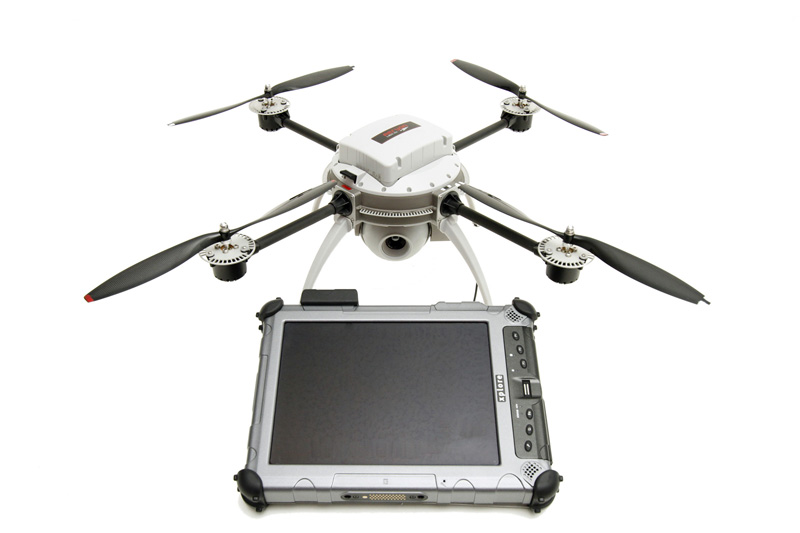
\includegraphics[width=11.0cm]{images/aeryon-scout-tablet.jpg}
\caption{The Aeryon Scout is a unmanned micro aerial vehicle, used for tactical, over-the-hill aerial intelligence. The platform is controlled by a touchscreen interface and is able to fly pre-planned flight paths using GPS positioning.}
\label{fig:introduction_aeryon_scout}
\end{figure}

A \textbf{micro aerial vehicle (MAV)} is a class of unmanned aerial vehicles (UAV).
Their small size allows a wide ringe of robotic applications, such as surveillance, inspection and search \& rescue.
Particularly interesting are small quadrotor helicopters, which are lifted and propelled by four rotors.
They offer great manouvrability and stability, making them ideal for indoor flights.
Due to technical developments in the last years, small quadrotors with on-board stabilization like the Parrot AR.Drone can be bought off-the-shelf.
These quadrotors make it possible to shift the research from basic control of the platform towards intelligent applications that require information about the surrounding environment.
However, the limited sensor suite and the fast movements make it quite a challenge to perform SLAM-like methods for such platforms.

%	\section{Versatile scouting capabilities of a quadrotor helicopter}


	\section{International Micro Air Vehicle Competition}
The international Micro Air Vehicle Competition (IMAV) is an effort to stimulate the practical demonstration of MAV technologies.
The competitions have as goal to shorten the road from novel scientific insights to application of the technology in the field.
Since the Summer 2011 edition of IMAV, teams can apply for borrowing a Parrot AR.Drone.
This allows teams to focus research on the artificial intelligence part of the competitions.

Currently, IMAV has three distinct competitions: two indoor competitions and one outdoor competition.
One of the indoor competitions is the Pylon challenge (Figure \ref{fig:imav2011_pylon}), which is often called the \textit{Figure-Eight challenge}.
The objective of the Pylon challenge is to navigate a MAV in figure-eight’s around two poles.
The competition rules\footnote{\url{http://www.imav2011.org/images/stories/documents/imav2011-summerediton_indoor_challenges_v3.0.pdf}} have been created to stimulate the level of autonomy; significantly more points are given to fully autonomous flights.

\begin{figure}[htb]
\centering
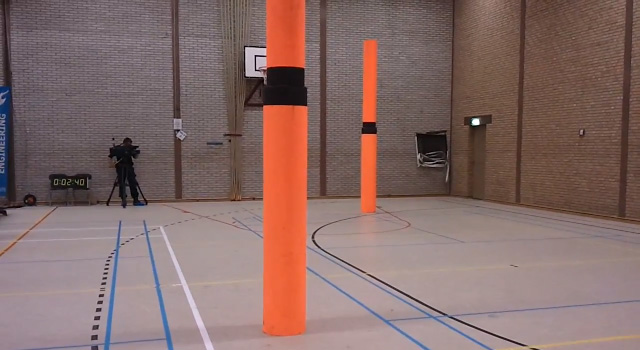
\includegraphics[width=11cm]{images/imav2011_pylon.jpg}
\caption{The IMAV2011 Pylon challenge environment, which is located in a sports gym.
The objective is to navigate a MAV in figure-eight’s around two poles that are $10\small{m}$ apart. Each pole has a height of approximately $4\small{m}$.}
\label{fig:imav2011_pylon}
\end{figure}

The main bottleneck for indoor autonomy is reliable indoor positioning.
Team are allowed to use external aids to solve their positioning problem, at the cost of points.
Examples of external aids are visual references, radio positioning beacons, etc.
This thesis is an effort to develop basic navigation capabilities for the AR.Drone, without relying on external aids.
These navigation capabilities can be used during the IMAV competitions, allowing fully autonomous flights.

	\section{RoboCup Rescue}
Another effort to promote research and development in robotics is RoboCup \cite{kitano1997robocup}.
The RoboCup competions have as goal to stimulate research by providing standard problems where wide range of technologies can be integrated and examined.
Unlike the IMAV competitions, the RoboCup competitions are not limited to MAVs.

The Robocup Rescue league is part of the Robocup initiative.
This league aims at the development of robotic technology that could effectively help human rescuers in the aftermath of disasters like earthquakes, terroristic attacks, and other extreme situations.
In addition to a Rescue league with real robots, the Virtual Robots Competition was started, which uses a simulator instead of real robots.
Simulation has some significant advantages above real competitions, such as the low costs and the ability to easily construct different disaster scenarios.

The main bottleneck for robot simulation is the requirement of realistic motion and sensor models.
The simulation environment selected for the Virtual Robots Competition is USARSim \cite{Balakirsky2009iros,carpin2007usarsim}, which includes models of a wide range of robotic platforms and sensors.
Unfortunately, the support of aerial vehicles in USARSim is little, while MAVs offer great advantages above other robots due to the versatile scouting capabilities.
In 2011, the expensive AirRobot quadrotor was the single aerial vehicle available in USARSim.
This thesis is an effort to develop a detailed model of the cheap AR.Drone quadrotor.
The resulting model can be used by teams to make use the advantages of MAVs in disaster scenarios.


	\section{Objectives and research questions}
An important goal of robotics is to develop mobile robots that can operate fully autonomously in real world situations.
One of the main prerequisites of an autonomous robot is the ability to known its location and movement in the environment.
Since no assumptions can be made about the environment, the robot has to learn from its environment.

Localization and mapping using aerial vehicles is an active research area in robotics.
However, current approaches use estimation and optimization algorithms that are computationally expensive and cannot be applied for realtime navigation problems.
Furthermore, other researchers rely on expensive aerial vehicles equipped with advanced sensors (e.g., laser range finder).
Focusing on realtime methods and cheap MAVs increases the employability of aerial vehicles in the real world situations.
In case of semi-autonomous robots, building and visualizing an elevated and textured map of the invironment offers additional feedback to the teleoperator of the vehicle.

The main research question therefore is to determine a realtime localization and mapping approach that can be used for MAVs with a low-resolution down-pointing camera (e.g., AR.Drone).
This main research question is divided into several subquestions:
\begin{itemize}
\item Is a very low-resolution camera (e.g., $176 \times 144$ pixels) sufficient for localization against a map?
\item Is localization on regular basis possible for circumstances encountered during the IMAV competition?
\item What is a robust/good method to estimate the transformation between frames and between a frame and a map?
\item How to construct an elevated and textured map with a single low-resolution camera and a single ultrasound sensor?
\item How useful are the produced visual maps for human navigation purposes?
\end{itemize}
The thesis goal is then to develop a novel approach that enables a MAV with a low-resolution down-looking camera to navigate in circumstances encountered during the IMAV competition.
In addition to the navigation capabilities, the approach generates an elevated and textured map of the environment, during flight.

	%\section{Contributions}
	\section{Outline}
\textbf{Chapter \ref{chapter:background-theory}} gives an overview of the background theory that is part of the presented methods.
This theory includes probabilistic robotics and computer vision techniques.
In \textbf{Chapter \ref{chapter:related-research}}, an overview of related research is given.
This reseach is divided into three segments: SLAM methods for building visual maps, elevation mapping with ultrasound sensors and research conducted with the AR.Drone.
An extensive overview of the AR.Drone platform is presented in \textbf{Chapter \ref{chapter:platform}}.
The platform overview covers the hardware, the basics of the quadrotor flight control and finally its Application Programming Interface (API).
However, the API lacks functionalities to employ a SLAM method.
Therefore, it is extended to a development framework in \textbf{Chapter \ref{chapter:development-environment}}.
In addition to this framework, a realistic simulation model of the AR.Drone is developed.
This simulation model allows safe and efficient development and testing of algorithms.
\textbf{Chapter \ref{chapter:visual-slam}} presents the Visual SLAM method for the AR.Drone.
It includes pose estimation, realtime  mapping, localization using the map and building an elevation map using a single ultrasound sensor.
\textbf{Chapter \ref{chapter:results}} describes the conducted experiments and presents the results.
The methods and results are discussed in depth in \textbf{Chapter \ref{chapter:discussion}}.
In \textbf{Chapter \ref{chapter:conclusions}}, this thesis concludes by answering the research questions and summarizing directions for future research.



%\chapter{Background theory}
%\label{chapter:background-theory}
%	\section{Probabilistic robotics}
		\subsection{Motion}
		\subsection{Vision}
		\subsection{Localization}
		\subsection{Solution techniques}

		%\subsection{Extended Kalman filter}
		%\subsection{Particle filter}
		%\subsection{Information filter}
	\section{Camera geometry}
		\subsection{Camera models}
			\subsubsection{Camera matrix}
		\subsection{Projective transformations}
	\section{Image stitching}
		\subsection{Feature detection}
			\subsubsection{SIFT}
			\subsubsection{SURF}
		\subsection{Feature matching}
		\subsection{Transformations}
			\subsubsection{Outlier detection}


\chapter{Probabilistic Robotics}
\label{chapter:probabilistic-robotics}
In Chapter 2 and 3, an introduction to background theory for this thesis is given.
The work presented in this thesis relies on \textbf{probabilistic robotics} (Thrun et al \cite{fox2005probabilistic}), which is introduced in this chapter.
The work also relies on \textbf{computer vision} (Hartley and Zisserman \cite{Hartley2004}), which is introduced in Chapter \ref{chapter:computer-vision}.
A clear vocabulary and corresponding mathematical nomenclature will be established that will be used consistently in the remainder of this thesis.
Probabilistic robotics uses the notation of Thrun et al \cite{fox2005probabilistic}.
%and computer vision uses the notation of Hartley and Zisserman \cite{Hartley2004}.

Sensors are limited in what they can perceive (e.g., the range and resolution is subject to physical limitations).
Sensors are also subject to noise, which deviates sensor measurements in unpredictable ways.
This noise limits the information that can be extracted from the sensor measurements.
Robot actuators (e.g., motors) are also subject to noise, which introduces uncertainty.
Another source of uncertainty is caused by the robot's software, which uses approximate models of the world.
Model errors are a source of uncertainty that has often been ignored in robots.
Robots are real-time systems, limiting the amount of computation that can be done.
This requires the use of algorithmic approximations, but increases the amount of uncertainty even more.

For some robotic applications (e.g., assembly lines with controlled environment), uncertainty is a marginal factor.
However, robots operating in uncontrolled environments (e.g., homes, other planets) will have to cope with significant uncertainty.
Since robots are increasingly deployed in the open world, the issue of uncertainty has become a major challenge for designing capable robots.
\textit{Probabilistic robots} is a relatively new approach to robotics that pays attention to the uncertainty in perception and action.
Uncertainty is represented explicitly using the calculus of probability theory.
This means that probabilistic algorithms represent information by probability distributions over a space.
This allows to represent ambiguity and degree of belief in a mathematically sound way.
Now, robots can make choices (plan) with respect to the uncertainty that remains, or chose to reduce the uncertainty (e.g., explore) if that is the best choice.

\section{Recursive state estimation}
\label{sec:background-recursive-state-estimation}
Environments are characterized by \textit{state}.
A state can be seen as a collection of all aspects of the robot and the environment that can impact the future.
The state also includes variables regarding the robot itself (e.g., pose, velocity, acceleration).
\begin{mydef}
Environments are characterized by \textbf{state}, which describes all aspects of a robot and the environment that can impact the future.
A state can be either \textbf{static state} (non-changing) or \textbf{dynamic state} where certain state variables tend to change over time.
A state is denoted $x$.
The state at time $t$ is denoted $x_t$.
\end{mydef}
Common state variables are:
\begin{itemize}
\item The robot \textit{pose}, which is its location and orientation relative to a global coodinate frame.
\item The \textit{robot velocity}, consisting of a velocity for each pose variable.%A change in attitude is called \textit{angular velocity}.
\item The \textit{location and features of surrounding objects in the environment}. The objects can be either \textit{static} or \textit{dynamic}. For some problems, the objects are modelled as \textit{landmarks}, which are distinct, stationary features that provide reliable recognition.
\end{itemize}

A core idea of probabilistic robotics is the estimation of the state from sensor data.
Sensors observe only partial information about those quantities and their measurements are affected by noise. 
State estimation tries to recover state variables from the data.
Instead of computing a single state, a probability distribution is computed over possible world states.
This probability distribution over possible world states is called \textit{belief} and is described on the next page.
\begin{mydef}
\textbf{State estimation} addresses the problem of estimating quantities (state variables) from sensor data that are not directly observable, but can be inferred.
A probability distribution is computed over possible world states.
\end{mydef}

A robot can \textbf{interact} with its environment by influencing the state of its environment through its actuators (\textit{control actions}), or it can gather information about the state through its sensors (\textit{environment sensor measurements}).
\begin{mydef}
$z_{t_1:t_2} = z_{t_1}, z_{t_1 + 1}, z_{t_1 + 2}, \hdots, z_{t_2}$ denotes the set of all \textbf{measurements} acquired from time $t_1$ to time $t_2$, for $t_1 \leq t_2$.
\end{mydef}
\begin{mydef}
$u_{t_1:t_2} = u_{t_1}, u_{t_1 + 1}, u_{t_1 + 2}, \hdots, u_{t_2}$ denotes the sequence of all \textbf{control data} from time $t_1$ to time $t_2$, for $t_1 \leq t_2$.
\end{mydef}
The control data conveys information regarding the change of state.
For example, setting a robot's velocity at $1 \small{m/s}$, suggests that the robot's new position after $2$ seconds is approximately $2$ meters ahead of its position before the command was executed.
As a result of noise, $1.9$ or $2.1$ meters ahead are also likely new positions.
Generally, measurements provide information about the environment's state, increasing the robot's knowledge.
Motion tends to induce a loss of knowledge due to the inherent noise in robot actuation and the stochasticity of the environment.

The evolution of state and measurements is performed by \textbf{probabilistic laws}.
State $x_t$ is generated stochastically from the state $x_{t-1}$.
If state $x$ is complete (i.e., best predictor of the future), it is a sufficient summary of all that happened in previous time steps.
This assumption is known as the \textit{Markov Assumption} and is expressed by the following equality:
%and implies the current knowledge is sufficient to represent the past history of the robot.
\begin{equation}
\label{eq:background_state_trans_prob}
p(x_t | x_{0:t - 1}, z_{1:t - 1}, u_{1:t}) = p(x_t | x_{t-1}, u_t)
\end{equation}
where $p(x_t | x_{t-1}, u_t)$ is called \textit{state transition probability} and specifies how environmental state evolves over time as a function of robot control $u_t$.
%The state at time $t$ is stochastically dependent on the state at time $t - 1$ and the control $u$.

\begin{mydef}
The \textbf{Markov Assumption} states that past and future data are independently if one knows the current state $x$. This means the values in any state are only influenced by the values of the state that directly preceded it.
\end{mydef}

The process by which measurements are modelled is expressed by:
\begin{equation}
\label{eq:background_measurement_prob}
p(z_t | x_{0:t}, z_{1:t-1}, u_{1:t}) = p(z_t | x_t)
\end{equation}
where $p(z_t | x_t)$ is called \textit{measurement probability} and specifies how measurements are generated from the environment state $x$.

Another core idea of probabilistic robotics is \textbf{belief}, which reflects the robot's knowledge about the environment's state.
Belief distributions are posterior probabilities over state variables conditioned on the available data.
The Markov Assumption implies the current belief is sufficient to represent the past history of the robot.
%Belief is represented through conditional probability distributions (posterior probabilities over state variables conditioned on the available data).
The belief over state variables is expressed with $bel(x_t)$:
%, which is an abbrevation for the posterior
\begin{equation}
bel(x_t) = p(x_t | z_{1:t}, u_{1:t})
\end{equation}
A \textit{prediction} of the state at time $t$ can be made before incorporating a measurement.
This prediction is used in the context of probabilistic filtering and is denoted as follows:
\begin{equation}
\overline{bel}(x_t) = p(x_t | z_{1:t-1}, u_{1:t})
\end{equation}
This equation predicts the state at time $t$ based on the previous state posterior, before incorporating the measurement at time $t$.
%A \textit{correction} or \textit{measurement update} is obtained by calculating $bel(x_t)$ from $\overline{bel}(x_t)$.

\begin{mydef}
\textbf{Belief} reflects the robot's knowledge about the environment's state, through conditional probability distributions.
Belief over state variable $x_t$ is denoted by $bel(x_t)$.
\end{mydef}

\subsection{Algorithms}
\label{sec:prob-rob-bayes}
The most general algorithm for calculcating beliefs is the \textbf{Bayes filter}.
The input of the algorithm is the (initial) belief $bel$ at time $t-1$, the most recent control $u_t$ and measurement $z_t$.
First, a \textit{prediction} for the new belief is computed based on control $u_t$ (the measurement is ignored):
\begin{equation}
\label{eq:background-theory-bayes-predict}
\overline{bel}(x_t) = \int p(x_t | u_t, x_{t-1}) bel(x_{t-1}) dx_{t-1}
\end{equation}
The second step of the Bayes filter is the \textit{measurement update}:
\begin{equation}
\label{eq:background-theory-bayes-measurement}
bel(x_t) = \eta p(z_t | x_t) \overline{bel}(x_t)
\end{equation}
Where $\eta$ is a normalization constant to ensure a valid probability.
Now, $bel(x_t)$ is the robot's belief about the state after the measurement and control data are used to improve the robot's knowledge.
Both steps of the algorithm are performed recursively for all measurements and controls.

The most popular family of recursive state estimators are the \textbf{Gaussian filters}.
Gaussian filters represent belief by multivariate normal distributions (approximated by a Gaussian function).
The density (probability) over the state space $x$ is characterized by two parameters: the mean $\mu$ and the covariance $\Sigma$.
The dimension of the covariance matrix is the dimensionality of the state $x$ squared.
Representing the posterior by a Gaussian has some important consequences.
First, Gaussians are unimodel and have a single maximum.
However, this is characterisic for many tracking problems, where the posterior is focussed around the true state with a certain margin of uncertainty.

In order to implement the filter described above, two additional components are required.
In Section \ref{sec:motion_model}, the \textit{motion model} is described.
In Section \ref{sec:measurement_model}, the \textit{measurement model} is described.

		\section{Motion model}
		\label{sec:motion_model}
Probabilistic motion models describe the relationship between the previous and current pose and the issued controls (commands) by a probability distribution. This is called the \textit{state transition probability}.
The state transition probability plays an essential role in the prediction step of the Bayes filter.
\begin{mydef}
A probabilistic \textbf{motion model} defines the state transition between two consecutive time steps $t-1$ and $t$ after a control action $u_{t}$ has been carried out. It is expressed by the posterior distribution $p (x_t | x_{t-1}, u_{t})$.
\end{mydef}
%In order to derive $p (x_t | x_{t-1}, u_{t})$, it is necessary to derive the kinematics from its mechanics and its %possible sources of noise and deviation.

Two complementary probabilistic motion models are the \textit{Velocity Motion Model} and the \textit{Odometry Motion Model}.
The Velocity Motion Model assumes that a robot is controlled through two velocities: a rotational velocity $\omega_t$ and translational velocity ($v_t$).
\begin{equation}
u_t = 
\left( \begin{array}{c}
v_t \\
\omega_t \end{array} \right)
\end{equation}
Algorithms for computing the probability $p (x_t | x_{t-1}, u_{t})$ can be found in \cite{fox2005probabilistic}.
The Odometry Motion Model assumes that one has access to odometry information (e.g., wheel encoder information).
In practice, odometry models tend to be more accurate, because most robots do not execute velocity command with the level of accuracy that is obtained by measuring odometry.
Technically, odometry readings are not controls because they are received after executing a command.
However, using odometry readings as controls results in a simpler formulation of the estimation problem.

Both motion models are not directly applicable to MAVs.
For example, quadrotor helicopters are controlled through pitch, roll and yaw (as explained in Section \ref{sec:platform-quadrotor-flight-control}).
A conversion between angles to velocities is required to use the Velocity Motion Model for a quadrotor helicopter.
For ground robots, the odometry reading can be obtained by integrating wheel encoder information.
Because a quadrotor helicopter has no contact with the ground, odometry readings are not directly available.
Instead, different sources of information are used to obtain odometry information.
For example, the AR.Drone uses a down-pointing camera to recover odometry information (Section \ref{sec:platform-visual-odometry}).


		\section{Measurement model}
		\label{sec:measurement_model}
Probabilistic measurement models describe the relationship between the world state $x_t$ and how a sensor reading (observation) $z_t$ is formed.
Based on the estimated world state $x_t$, a belief over possible measurements is generated.
Noise in the sensor measurements is modelled explicitly, inherent to the the uncertainty of the robot's sensors.
To express the process of generating measurements, a specification of the environment is required.
A map $m$ of the environment is a list of objects and their locations:
\begin{equation}
m = \{m_1, m_2, \hdots, m_N\}
\end{equation}
Where $N$ is the total number of objects in the environment.
Maps are often \textit{Features-based maps} or \textit{Location-based maps}.
Location-based maps are volumetric and offer a label for any location.
Features-based maps only describe the shape of the environment at specific locations, which are commonly objects.
Features-based maps are more popular because the representation makes it easier to adjust (refine) the position of objects.
\begin{mydef}
A probabilistic \textbf{sensor model} describes the relation between a world state $x_t$ and a sensor reading $z_t$ given an environmental model $m$ in form of a posterior distribution $p (z_t | x_t, m)$.
\end{mydef}


		\section{Localization}
\label{sec:probabilistic-robotics-localization}
\textit{Robot localization} is the problem of estimating the robot's pose (state) relative to a map of the environment.
Localization is an important building block for successful navigation of a robot, together with \textit{perception}, \textit{cognition} and \textit{motion control}.

When a robot is moving in a known enviroment and starting at a known location, it can keep track of its location by integrating local position estimates (e.g., odometry).
Due to uncertainty of these local estimates, the uncertainty of the robot's absolute location increases over time.
In order to reduce the growing uncertainty, the robot has to retrieve its absolute location by localizing itself in relation to a map.
To do so, the robot uses its sensors to make observations of its environment and relate these observations to a map of the environment.

A probabilistic approach to localization uses belief to represent the estimated global location.
Again, updating the robot's position involves two steps.
The first step is called the \textit{prediction update}.
The robot uses its state at time $t - 1$ and control data $u_t$ to predicts its state at time $t$.
This prediction step increases the uncertainty about the robot's state.
%The uncertainty about the robot's state increases due to integration of the odometric error over time.
The second step is called the \textit{perception update}.  
In this step, the robot uses the information from its sensors to correct the position estimated during the prediction phase, reducing the uncertainty about the robot's state.

\section{Simultaneous Localization and Mapping}
\label{sec:probabilistic-robotics-slam}

A more difficult subclass of localization occurs when a map of the environment is not available.
In this case, the robot's sensor information is used to both recover the robot's path and build a map of the environment.
In the robotics community, this problem is called \textbf{Simultaneous Localization and Mapping (SLAM)}.
A solution to this problem would make a robot truly autonomous.
SLAM is a difficult problem because both the estimated path and constructed map are affected by noise.
Both of them become increasingly inaccurate during travel.
However, when a place that has been mapped is revisited, the uncertainty can be reduced.
This process is called \textit{loop-closing}.
Additionally, the map can be optimized after a loop-closure event is detected.


\subsection{Solution techniques}
\label{sec:background-solution-techniques}
In practice, it is not possible to compute a robot's belief (posterior probabilities) analytically.
%the posterior (belief) analytically.
Therefore, a number of approximation techniques exist. 
This section describes the most popular solution techniques for SLAM problems.

Solution techniques can be divided in two major branches of belief representation: \textit{Single-hypothesis belief} and \textit{Multi-hypothesis belief}.
\textbf{Single-hypothesis trackers} represent belief by a single world state.
This estimate is associated by a measure of certainty (or variance), allowing the tracker to broaden or narrow the estimated region in the state space.
The main advantage of the single-hypothesis representation is the absence of ambiguity, simplifying decision-making at the robot's cognitive level (e.g., pathplanning).
Due to the absence of ambiguity, the trackers fail to model ambiguities adequately.
%An example is a soccer field, which is a symmetrical environment.

\textbf{Multi-hypothesis trackers} represent belief not just as a single world state, but as a possibly infinite set of states.
The main advantage of the multi-hypothesis representation is that the robot can explicitly maintain uncertainty regarding its state.
This allows a robot to believe in multiple poses simultaneously, allowing the robot to track and reject different hypotheses independently.
One of the main disadvantages of a multi-hypothesis representation involves decision making.
If the robot represents its position as a set of points, it becomes less obvious to compute a next action.

Futhermore, solution techniques can be divided in two branches of time constraints: \textit{online computing} and \textit{offline computing}.
\textbf{Online} techniques solve a problem in real-time and must guarantee response within strict time constraints.
One advantage of online techniques is the ability to use the response as input for decision making (e.g., navigation), which is essential for autonomous robots.
Due to the strict time constraints, a limited amount of computations can be performed, which limits the complexity of solution techniques.

\textbf{Offline} techniques have less strict time constraints, which allow increased complexity.
For example, additional refinements or optimizations can be performed that would be too slow for online techniques.
One of the main disadvantages of offline techniques involves decision making.
Because a response is not available in real-time, the robot has to wait or make a decision without incorporating the response.


\subsubsection{Kalman Filter (KF)}
\label{sec:prob-rob-kf}
The most popular technique for implementing a Bayes filter is probably the Kalman Filter (1960) \cite{kalman1960new}, often used for improving vehicle navigation.
The filter has a Single-hypothesis belief representation and can be performed in real-time.
The Kalman Filter is based on the assumption that the system is linear and both the motion model and measurement model are affected by white Gaussian noise.
Belief at time $t$ is represented by a multivariate Gaussian distribution defined by its mean $\mu_t$ and covariance $\Sigma_t$.
This means the $x_t$ from the Bayes filter (Equations \eqref{eq:background-theory-bayes-predict} and \eqref{eq:background-theory-bayes-measurement}) has been replaced by $\mu_t$ and $\Sigma_t$.
%This representation limits the filter to continuous states.

The Kalman Filter assumes the system is linear: the state transition $A$ (Equation \ref{eq:background_state_trans_prob}), the motion model $B$ and the sensor model $C$ (Equation \ref{eq:background_measurement_prob}) are linear functions solely depending on the state $x$ or control command $u$, plus a Gaussian noise model $Q$:
\begin{equation}
\label{eq:KF}
\begin{array}{rclr}
\text{\textbf{Predict}} \\
\overline{\mu}_t & = & A_t \mu_{t-1} + B_t u_t  & \text{a-priori mean estimate} \\
\overline{\Sigma}_t & = & A_t \Sigma_{t-1} A_t^T + R_t  & \text{a-priori covariance estimate} \\
\text{\textbf{Update}} \\
K_t & = & \overline{\Sigma}_t C_t^T (C_t \overline{\Sigma}_t C_t^T + Q_t)^{-1} & \text{Kalman gain} \\
\mu_t & = & \overline{\mu}_t + K_t(z_t - C_t \overline{\mu}_t) & \text{updated (a posteriori) state estimate} \\
\Sigma_t & = & (I - K_t C_t) \overline{\Sigma}_t & \text{updated (a posteriori) estimate covariance}
\end{array}
\end{equation}

The Kalman Filter represents the belief $bel(x_t)$ at time $t$ by the mean $\mu_t$ and covariance $\Sigma_t$.
When a measurement is received, a new belief $bel(x_t)$ is predicted based on the previous belief bel($x_{t-1}$), the control data $u_t$ and both the state transition model and motion model.
This predicted belief describes the most likely state $\overline{\mu}_t$ at time $t$ and the covariance $\overline{\Sigma}_t$.
The measurement is not yet included, because it is a predicted belief.
The update step transforms the predicted belief ($\overline{\mu}_t$, $\overline{\Sigma}_t$) into the desired belief ($\mu_t$, $\Sigma_t$), by incorporating the measurement $z_t$.
The Kalman gain $K_t$ specifies the degree to which the measurement is incorporated into the new state estimate.
The key concept used for Kalman Filtering is the \textit{innovation}, which is the difference between the actual measurement $z_t$ and the expected measurement $C_t \overline{\mu}_t$, which is derived from the predicted state.
A measurement $z_t$ which is far off the predicted measurement, is less reliable, thus less incorporated in the new state estimate.

The standard Kalman Filter requires a linear system (i.e., a linear combination of Gaussians results in another Gaussian), which is insufficient to describe many real-life problems.
Therefore, variations of the original algorithm have been proposed that can cope with different levels of non-linearity.
These variations approximate the motion and sensor models in a way to make them linear again.

\subsubsection{Extended Kalman Filter (EKF)}
The Extended Kalman Filter is a variant on the Kalman Filter that can be used for non-linear systems.
It tries to approximate \textit{non-linear} motion and sensor models to make them linear.
The state transition probability and the measurement probabilities are governed by the non-linear functions $g$ and $h$:
\begin{equation}
\begin{array}{rcl}
x_t & = & g(u_t, x_{t-1}) \\
z_t & = & h(x_t) + \delta_t
\end{array}
\end{equation}
These functions replace $A$, $B$ and $C$ of the regular Kalman Filter (Equation \ref{eq:KF}).

They key idea of the EKF approximation is called \textit{linearization}.
A first-order linear Taylor approximation is calculated at the mean of the current belief (Gaussian), resulting in a linear function.
Projecting the Gaussian belief through the linear approximation results in a Gaussian density.
\begin{equation}
\begin{array}{rclr}
\text{\textbf{Predict}} \\
\overline{\mu}_t & = & \boldsymbol{g(u_t, \mu_{t-1})} & \text{a-priori mean estimate} \\
\overline{\Sigma}_t & = & \boldsymbol{G_t} \Sigma_{t-1} \boldsymbol{G_t^T} + R_t  & \text{a-priori covariance estimate} \\
\text{\textbf{Update}} \\
K_t & = & \overline{\Sigma}_t \boldsymbol{H_t^T} (\boldsymbol{H_t} \overline{\Sigma}_t \boldsymbol{H_t^T} + Q_t)^{-1} & \text{Kalman gain} \\
\mu_t & = & \overline{\mu}_t + K_t(z_t - \boldsymbol{h(\overline{\mu}_t)}) & \text{updated (a posteriori) state estimate} \\
\Sigma_t & = & (I - K_t \boldsymbol{H_t}) \overline{\Sigma}_t & \text{updated (a posteriori) estimate covariance}
\end{array}
\end{equation}



\subsubsection{TORO}
\label{sec:prob-rob-toro}
As stated in Section \ref{sec:probabilistic-robotics-slam}, both the estimated path and constructed map are affected by noise.
Both of them become increasingly inaccurate during travel.
However, when a place that has been mapped is revisited (loop-closure), the uncertainty can be reduced and the map can be optimized to reduce its error.
This optimization procedure is computationally expensive since it needs to search for a configuration that minimizes the error of the map.

A solution technique for the map optimization problem is TORO \cite{grisetti2007efficient}. This technique is used in a comparable setting (visual SLAM with a MAV), as described in Section \ref{sec:realted-visual-slam-steder}.
The TORO algorithm operates on a graph-based formulation of the SLAM problem, in which the poses of the robot are modeled by nodes in a graph.
Constraints between poses resulting from observations or from odometry are encoded in the edges between the nodes.
The goal of TORO is to find a configuration of the nodes that maximizes the observation likelihood encoded in the constraints.
Gradient Descent (GD) \cite{olson2006fast} seeks for a configuration of the nodes that maximizes the likelihood of the observations by iteratively selecting an edge (constraint) $< j, i >$ and by moving a set of nodes
%of the network
in order to decrease the error introduced by the selected constraint.

\begin{comment}
The nodes are updated according to the following equation: 
\begin{equation}
x^{t + 1} = x^t + \Delta x
%\lambda \cdot J_{ji}^T \Omega_{ji} r_{ji}
\end{equation}
where $x$ is the set of variables describing the locations of the poses in the network, and the term $\Delta x$ is used to move a node in the direction that decreases the error.
The direction of $\Delta x$ is computed from the residual (opposite of the error vector) scaled by the information encoded in the contraint.
In practice, GD decomposes the overall problem into many smaller problems by optimizing the constraints individually.
\end{comment}

The TORO algorithm uses a tree based parameterization for describing the configuration of the nodes in the graph.
%Such a tree can be obtained by computing a spanning tree from a graph.
Such a tree can be constructed from trajectory of the robot.
The first node is the root of the tree.
An unique id is assigned to each node based on the timestamps of the observations.
Furthermore, the parent of a node is the node with the smallest id (timestamp) and a constraint between both nodes.
Each node $i$ in the tree is related to a pose $p_i$ in the network and maintains a parameter $x_i$.
The parameter $x_i$ is a 6D vector and describes the relative movement (rotation and translation) from the parent of node $i$ to  node $i$ itself.
%\begin{equation}
%x_i = p_i \ominus p_{parent(i)}
%\end{equation}
The pose of a node can be expressed as:
\begin{equation}
P_i = \prod_{k \in \mathcal{P}_{i,0}} X_k
\end{equation}
Where $\mathcal{P}_{i,0}$ is the ordered list of nodes describing a path in the tree from the root to node $i$.
The homogenous transformation matrix $X_i$ consists of a rotational matrix $R$ and a translational component $t$.

Distributing an error $\epsilon$ over a sequence of $n$ nodes in the two-dimensional space can be done in a straightforward manner.
For example, by changing the pose of the $i$-th node in the chain by $\frac{i}{n} \times r^{2D}$.
In the three-dimensional space, such a technique is not applicable.
The reason for that is the non-commutativity of the three rotations.
The goal of the update rule in GD is to iteratively update the configuration of a set of nodes in order to reduce the error introduced by a constraint.

The error introduced by a constraint is computed as follows:
\begin{equation}
E_{ji} = \Delta_{ji}^{-1} P_i^{-1} P_j
\end{equation}
In TORO's approach, the error reduction is done in two steps.
First, it updates the rotational components $R_k$ of the variables $x_k$ and second, it updates the translational components $t_k$.
The orientation of pose $p_j$ is described by:
\begin{equation}
\mathcal{R}_1\mathcal{R}_2 \hdots \mathcal{R}_n = \mathcal{R}_{1:n}
\end{equation}
where $n$ is the length of the path $\mathcal{P}_{ji}$.
The error can be distributed by determining a set of increments in the intermediate rotations of the chain so that the orientation of the last node $j$ is $\mathcal{R}_{1:n} B$. Here $B$ is a matrix that rotates $x_j$ to the desired orientation based on the error.
Matrix $B$ can be decomposed into a set of incremental rotations $B = B_{1:n}$.
The individual matrices $B_k$ are computed using a spherical linear interpolation (slerp) \cite{barrera2004incremental}.

The translational error is distributed by linearly moving the individual nodes along the path by a fraction of the error.
This fraction depends on the uncertainty of the individual constraints (encoded in the corresponding covariance matrices).

Despite TORO is presented as an efficient estimation method, it cannot solve realistic problems in real-time \cite{grisetti2007efficient}, which makes it an offline solution technique.
All work presented in this thesis has a strong emphasis on online techniques, which allows the work to be used for navigation tasks like the IMAV Pylon challenge (Section \ref{sec:introduction-imav}).
For this reason, a TORO-based optimization algorithm was not used in this thesis.
Furthermore, a single-hypothesis belief representation was chosen for its simplicity.


\begin{comment}
\subsection{Single-hypothesis trackers}
Single-hypothesis trackers represent belief by a single world state.
This estimate is associated by a measure of certainty (or variance), allowing the tracker to broaden or narrow the estimated region in the state space.
The main advantage of the single-hypothesis representation is the absence of ambiguity, simplifying decision-making at the robot's cognitive level (e.g., pathplanning).
Updating the robot's belief is also simplified, because a single state must be updated to a new single state.
However, the main disadvantage of a single-hypothesis representation is that a update process always has to generate a \textit{single} hypothesis, which is challenging and sometimes impossible.

\paragraph{Kalman Filter (KF)}
The most popular technique for implementing a Bayes filter is probably the Kalman Filter (1960) \cite{kalman1960new}, often used for improving vehicle navigation.
The Kalman Filter is based on the assumption that the system is linear and both the motion model and measurement model are affected by white Gaussian noise.
Belief at time $t$ is represented by a multivariate Gaussian distribution defined by its mean $\mu_t$ and covariance $\Sigma_t$.
This representation limits the filter to continuous states.

The Kalman Filter assumes the system is linear: the state transition $A$ (Equation \ref{eq:background_state_trans_prob}), the motion model $B$ and the sensor model $C$ (Equation \ref{eq:background_measurement_prob}) are linear functions solely depending on the state $x$ or control command $u$, plus a Gaussian noise model $Q$:
\begin{equation}
\label{eq:KF}
\begin{array}{rclr}
\text{\textbf{Predict}} \\
\overline{\mu}_t & = & A_t \mu_{t-1} + B_t u_t  & \text{a-priori mean estimate} \\
\overline{\Sigma}_t & = & A_t \Sigma_{t-1} A_t^T + R_t  & \text{a-priori covariance estimate} \\
\text{\textbf{Update}} \\
K_t & = & \overline{\Sigma}_t C_t^T (C_t \overline{\Sigma}_t C_t^T + Q_t)^{-1} & \text{Kalman gain} \\
\mu_t & = & \overline{\mu}_t + K_t(z_t - C_t \overline{\mu}_t) & \text{updated (a posteriori) state estimate} \\
\Sigma_t & = & (I - K_t C_t) \overline{\Sigma}_t & \text{updated (a posteriori) estimate covariance}
\end{array}
\end{equation}

The Kalman Filter presesents the belief $bel(x_t)$ at time $t$ by the mean $\mu_t$ and covariance $\Sigma_t$.
When a measurement is received, a new belief $bel(x_t)$ is predicted based on the previous belief bel($x_{t-1}$), the control data $u_t$ and both the state transition model and motion model.
This predicted belief describes the most likely state $\overline{\mu}_t$ at time $t$ and the covariance $\overline{\Sigma}_t$.
The measurement is not yet included, because its a predicted belief.
The update step transforms the predicted belief ($\overline{\mu}_t$, $\overline{\Sigma}_t$) into the desired belief ($\mu_t$, $\Sigma_t$), by incorporating the measurement $z_t$.
The Kalman gain $K_t$ specifies the degree to which the measurement is incorporated into the new state estimate.
The key concept used for Kalman Filtering is the \textit{innovation}, which is the difference between the actual measurement $z_t$ and the expected measurement $C_t \overline{\mu}_t$, which is derived from the predicted state.
A measurement $z_t$ which is far off the predicted measurement, is less reliable, thus less incorporated in the new state estimate.

The standard Kalman Filter requires a linear system (.i.e, a linear combination of Gaussians results in another Gaussian), which is insufficient to describe many real-life problems.
Therefore, variations of the original algorithm have been proposed that can cope with different levels of non-linearity.
These variations approximate the motion and sensor models in a way to make them linear again.

\paragraph{Extended Kalman Filter (EKF)}
The Extended Kalman Filter is a variant on the Kalman Filter that can be used for non-linear systems.
It tries to approximate \textit{non-linear} motion and sensor models to make them linear.
The state transition probability and the measurement probabilities are governed by the non-linear functions $g$ and $h$:
\begin{equation}
\begin{array}{rcl}
x_t & = & g(u_t, x_{t-1}) \\
z_t & = & h(x_t) + \delta_t
\end{array}
\end{equation}
These functions replace $A$, $B$ and $C$ of the regular Kalman Filter (Equation \ref{eq:KF}).

They key idea of the EKF approximation is called \textit{linearization}.
A first-order linear Taylor approximation is calculated at the mean of the current belief (Gaussian), resulting in a linear function.
Projecting the Gaussian belief through the linear approximation results in a Gaussian density.
\begin{equation}
\begin{array}{rclr}
\text{\textbf{Predict}} \\
\overline{\mu}_t & = & \boldsymbol{g(u_t, \mu_{t-1})} & \text{a-priori mean estimate} \\
\overline{\Sigma}_t & = & \boldsymbol{G_t} \Sigma_{t-1} \boldsymbol{G_t^T} + R_t  & \text{a-priori covariance estimate} \\
\text{\textbf{Update}} \\
K_t & = & \overline{\Sigma}_t \boldsymbol{H_t^T} (\boldsymbol{H_t} \overline{\Sigma}_t \boldsymbol{H_t^T} + Q_t)^{-1} & \text{Kalman gain} \\
\mu_t & = & \overline{\mu}_t + K_t(z_t - \boldsymbol{h(\overline{\mu}_t)}) & \text{updated (a posteriori) state estimate} \\
\Sigma_t & = & (I - K_t \boldsymbol{H_t}) \overline{\Sigma}_t & \text{updated (a posteriori) estimate covariance}
\end{array}
\end{equation}

\paragraph{Unscented Kalman Filter (UKF)}
A drawback of the Extended Kalman Filter is that the true mean and covariance of the posterior distribution is not preserved.
Another variant on the Kalman Filter has been found to yield superior results.
The \textit{Unscented Kalman Filter (UKF)} performs a stochastic linearization using a weighted statistical linear regression process.
The \textit{unscented transform} sampling technique is used to pick a minimal set of sigma points around the mean.
These sigma points are propagated through the non-linear function $g$, from which the mean and covariance of the estimate are then recovered.
Each sigma point has two weights associated with it. One weight is for recovering the mean, the other weight is used for recovering the covariance.

In practice, the EKF is sightly faster than the UKF.
The UKF produces better results than the EKF, depending on the non-linearities and spread of the prior state uncertainty.
However, in many practical applications, the different is very small.


\paragraph{Information Filter (IF)}
The dual of the Kalman Filter is the \textit{Information Filter}.
The key different between both filters lies in the way the Gaussian belief is represented.
Kalman Filters respresent Gaussians by their moments (mean and covariance).
Information Filters present Gaussians by their canonical parameterization (information matrix and information vector).
\begin{equation}
\label{eq:KF}
\begin{array}{rclr}
\text{\textbf{Predict}} \\
\overline{\Omega}_t & = & (A_t \Omega_{t-1}^{-1} A_t^T + R_t)^{-1}  & \text{a-priori information matrix} \\
\overline{\xi}_t & = & \overline{\Omega}_t ( A_t \Omega_{t-1}^{-1} \xi_{t-1} + B_t u_t )  & \text{a-priori information vector} \\
\text{\textbf{Update}} \\
\Omega_t & = & \C_t^T Q_t^{-1} \C_t + \overline{\Omega}_t & \text{updated information matrix} \\
\xi_t & = & C_t^T Q_t^{-1} z_t + \overline{\xi}_t & \text{updated information vector}
\end{array}
\end{equation}

The difference in parameterization leads to different computational complexities.
The prediction step of the Kalman Filter is additive, which makes is computationally inexpensive.
However, the measurement update in Kalman Filter is computationally complex, due to the requirement of matrix inversion.
For the Information Filter, the complexities are exactly opposite.
The prediction step of the Information Filter involves the inversion of two matrices, which can be complex.
On the other hand, the measurement update of the Information Filter is additive, which makes it inexpensive.
The main advantage of the Information Filter is that $N$ measurements can be filtered at each timestep simply by summing their information matrices and vectors.
This makes Information Filters particularly interesting for scenarios where multiple robots have to merge their local information with the information collected by other robots.


\begin{comment}
\subsection{Multi-hypothesis trackers}


\paragraph{Particle Filter}
The key idea of the \textit{Particle Filter}  is to represent the posterior $bel(x_t)$ by a set of random state particles (samples) drawn from this posterior.
This representation is approximate, but can represent a much broader space of discributions than the single-hypothesis trackers.
Another advantage is that the transformations are not limited to linear functions anymore.

The particles (samples) are denoted
\begin{equation}
\chi = x_t^{[1]}, x_t^{[2]}, \hdots, x_t^{[M]}
\end{equation}
Each particle $x_t^{[m]}$ is a state hypothesis at time $t$.
Ideally, the likelihood for a state hypothesis $x_t$ to be in $\chi$, should be proportional to $bel(x_t)$.
The denser a subregion of the the space is populated with particles, the more likely it is that the true state falls into this region.
In the prediction step, the motion model is applied to each particle $x_{t-1}^{[m]}$ to generate a prediction $x_t^{[m]}$.
When observation $z_t$ is made, the \textit{importance factor} $w_t^{[m]}$ is computed.
\begin{equation}
w_t^{[m]} = p ( z_t | x_t^{[m]}, z_{0 \to t-1})
\end{equation}
The final step of the particle filter is {resampling}, in which the current set of particles re-sampled based on the computed likelihoods.
The algorithm draws with replacement $M$ particles from the temporary set $\overline{\chi}_t$.
The probability of each particle is given by its importance weights.
This changes the distribution of the particle from $\overline{bel}(x_t)$ to $bel(x_t)$.

Particle filters overcome the limitations of using a Gaussian to represent a probability distribution.
With sufficient samples, they approach the Bayesian optimal estimate, so they can be made more accurate than either the EKF or UKF.
The increased representational power of particle filters comes at the cost of higher computational complexity.
And, when the number of particles is unsufficient, the particle filter might suffer from sample impoverishment.
\end{comment}

The theory described in this chapter is used in the work presented in Section \ref{chapter:visual-slam}.
Section \ref{sec:pose_estimation} describes the Kalman Filter and both the motion model and measurement model.


\chapter{Computer Vision}
\label{chapter:computer-vision}
In this chapter, the introduction to required background theory for this thesis is continued.
This chapter introduces \textbf{computer vision} (Hartley and Zisserman \cite{Hartley2004}).
A clear vocabulary and corresponding mathematical nomenclature will be established that will be used consistently in the remainder of this thesis.
Computer vision uses the notation of Hartley and Zisserman \cite{Hartley2004}.

Laser range scanners are often used for robot localization.
However, this sensor has a number of problems (e.g., limited range, deal with dynamic environments).
Vision has long been advertised as a solution.
A camera can make a robot perceive the world in a way similar to humans.
\textbf{Computer vision} is a field that includes methods for acquiring, processing, analyzing and understanding images.
Since a camera is the AR.Drone's only sensor capable of retrieving detailed information of the environment, computer vision techniques are essential when performing robot localization with the AR.Drone.
%In addition, vision techniques can be used to calibrate other sensors of a robot.

\section{Projective geometry}
\label{sec:background-projective-geometry}
Projective geometry describes the relation between a scene and how a picture of it is formed.
A projective transformation is used to map objects into a flat picture.
This transformation preserves straightness.
Multiple geometrical systems can be used to describe geometry.

\textbf{Euclidean geometry} is a popular mathematical system.
A point in Euclidean 3-space is represented by an unordered pair of real numbers, $(x, y, z)$.
However, this coordinate system is unable to represent vanishing points.
The \textit{Homogeneous coordinate system} is able to represent points at infinity.
Homogeneous coordinates have an additional coordinate.
Now, points are represented by \textit{equivalance classes}, where points are equivalent when they differ by a common multiple.
For example, $(x, y, z, 1)$ and $(2x, 2y, 2z, 2)$ represent the same point.
Points at infinity are represented using $(x, y, z, 0)$, because $(x/0, y/0, z/0)$ is infinite.
In Euclidean geometry, one point is picked out as the \textit{origin}.
A coordinate can be transformed to another coordinate by translating and rotating to a different position.
This operation is known as a \textbf{Euclidian transformation}.
A more general type of transformation is the \textbf{affine transformation}, which is a linear transformation (linear stretching), followed by a Euclidian transformation.
The resulting transformation performs moving (translating), rotating and
%finally
stretching linearly.
% possibly by different ratios in different directions.

In computer vision problems, projective space is used as a convenient way of representing the real 3D world.
A \textbf{projective transformation} of projective space $\mathds{P}^n$ is represented by a linear transformation of homogeneous coordinates:
\begin{equation}
X' = H_{(n+1)} \times _{(n+1)}X
\end{equation}
where $X$ is a coordinate vector, $H$ is a non-singular matrix and $X'$ is a vector with the transformed coordinates.

In order to analyze and manipulate images, understanding about the image formation process is required.
Light from a scene reaches the camera and passes through a lens before it reaches the sensor.
The relationship between the distance to an object $z$ and the distance behind the lens $e$ at which a focused image is formed, can be expressed as:
\begin{equation}
\label{eq:optics}
\frac{1}{f} = \frac{1}{z} + \frac{1}{e}
\end{equation}
where $f$ is the focal length.

The \textbf{pinhole camera} has been the first known example of a camera \cite{gernsheim1969history}.
%\footnote{\url{http://inventors.about.com/od/pstartinventions/a/stilphotography.htm}}
It is a lightproof box with a very small aperture instead of a lens.
Light from the scene passes through the aperture and projects an \textit{inverted image} on the opposite side of the box.
This principle has been adopted as a standard model for perspective cameras.
In this model, the \textit{optical center} $C$ (aperture) corresponds to the center of the lens.
The intersection $O$ between the optical axis and the image plane is called \textit{principal point}.
The pinhole model is commonly described with the image plane between $C$ and the scene in order to preserve the same orientation as the object.

The operation performed by the camera is called the \textbf{perspective transformation}.
It transforms the 3D coordinate of scene point $P$ to coordinate $p$ on the image plane.
A simplified version of the perspective transformation can be expressed as:
\begin{equation}
\frac{f}{P_z} = \frac{p_x}{P_x} = \frac{p_y}{P_y}
\end{equation}
from which $p_x$ and $p_y$ can be recovered:
\begin{equation}
p_x = \frac{f}{P_z} \cdot P_x
\end{equation}
\begin{equation}
p_y = \frac{f}{P_z} \cdot P_y
\end{equation}
When using homogeneous coordinates, a linear transformation is obtained:
\begin{equation}
\left[ \begin{array}{c}
\lambda p_x \\
\lambda p_y \\
\lambda
\end{array} \right]
=
\left[ \begin{array}{c}
f P_x \\
f P_y \\
P_z
\end{array} \right]
=
\left[ \begin{array}{c c c c}
f & 0 & 0 & 0  \\
0 & f & 0 & 0 \\
0 & 0 & 1 & 0
\end{array} \right]
\left[ \begin{array}{c}
P_x \\
P_y \\
P_z \\
1
\end{array} \right]
\end{equation}
From this equation can be seen that it is not possible to estimate the distance to a point (i.e., all points on a line project to a single point on the image plane).

A more realistic camera model is called the \textbf{general camera model}.
It takes into account the rigid body transformation between the camera and the scene, and \textit{pixelization} (i.e., shape and position of the camera's sensor).
Pixelization is addressed by replacing the focal length matrix with a \textit{camera intrinsic parameter matrix} $A$.
The rigid body transformation is addressed by adding a combined rotation and translation matrix $[R|t]$, which are called the \textit{camera extrinsic parameters}.
\begin{equation}
\lambda p = A [ R | t] P
\end{equation}
or
\begin{equation}
\left[ \begin{array}{c}
\lambda p_x \\
\lambda p_y \\
\lambda
\end{array} \right]
=
\left[ \begin{array}{c c c}
\alpha_u & 0 & u_0 \\
0 & \alpha_v & v_0 \\
0 & 0 & 1
\end{array} \right]
\left[ \begin{array}{c c c c}
r_{11} & r_{12} & r_{13} & t_1 \\
r_{21} & r_{22} & r_{23} & t_2 \\
r_{31} & r_{32} & r_{33} & t_3
\end{array} \right]
\left[ \begin{array}{c}
P_x \\
P_y \\
P_z \\
1
\end{array} \right]
\end{equation}

\textbf{Camera calibration} is the process of measuring the intrinsic and extrinsic parameters of the camera.
As explained in the previous paragraph, these parameters are required to calculate the mapping between 3D scene points to 2D points on the image plane.
When scene points $P$ and image points $p$ are known, it is possible to compute $A$, $R$, $t$ by solving the perspective projection equation.
Newer camera calibration techniques use a planar grid (e.g., chessboard-like pattern) instead of 3D points, to ease the extraction of corners.
The method requires several pictures of the pattern shown at different positions and orientations.
Because the 2D positions of the corners are known and matched between all images, the intrinsic and extrinsic parameters are determined simultaneously by applying a least-square minimization.

\section{Feature extraction and matching}
\label{sec:computer-vision-feature-extraction-matching}
In order to perform robot localization using vision sensors, the robot must be able to relate recent camera frames to previously received camera frames (map).
However, all measurements have an error, which complicates the matching.
A strategy to deal with uncertainty is by generating a higher-level description of the sensor data instead of using the raw sensor data.
This process is called \textit{feature extraction}.

\begin{mydef}
\textbf{Features} are recognizable structures of elements in the environment.
They are extracted from measurements and described in a mathematical way.
\textit{Low-level features} are geometric primitives (e.g., lines, points, corners) and \textit{high-level features} are objects (e.g., doors, tables).
\end{mydef}

Features play an essential role %
in the software of mobile robots.
They enable more compact and robust descriptions of the environment.
Choosing the appropriate features is a critical task when designing a mobile robot.

\subsection{Feature extraction}
\label{sec:background-feature-extraction}
A local feature is a small image patch that is different than its immediate neighborhood.
Difference can be in terms of intensity, color and texture.
Commonly, features are edges, corners or junctions.
The most important aspect of a feature detector is \textit{repeatability}, which means the detector is able to detect the same features when multiple images (with different viewing and illumination conditions) of the same scene are used.
Another important aspect of a feature detector is \textit{distinctiveness}, which means the information carried by a patch is distinctive as possible.
This is important for robust feature matching.
A good feature is \textit{invariant}, meaning that changes in camera viewpoint, illumination, rotation and scale do not affect a feature and its high-level description.

\textbf{Scale-invariant feature transform (SIFT)} \cite{lowe1999object} is probably the most popular feature extractor.
It is invariant to scale, rotation, illumination and viewpoint.
The algorithm can be outlined as follows.
First, an internal representation of an image is computed to ensure scale invariance.
Secondly, an approximation of the Laplacian of Gaussian is used to find interesting keypoints.
Third, keypoints are found at maxima and minima in the Difference of Gaussian from the previous step.
Fourth, bad keypoints (e.g., edges and low contrast regions) are eliminated.
Fifth, an orientation is calculated for each keypoint.
Any further calculations are done relative to this orientation, making it rotation invariant.
Finally, a high-level representation is calculated to uniquely identify features.
This \textit{feature descriptor} is a vector of 128 elements, containing orientation histograms.

For some applications or mobile platforms, the SIFT extractor is too slow.
Therefore, faster variants are proposed, like \textbf{Speeded Up Robust Feature (SURF)} \cite{Bay2008cviu}.
%SURF is partly inspired by the SIFT descriptor.
The standard version of SURF is several times faster than SIFT and claimed by its authors to be more robust against different image transformations than SIFT.
The important speed gain is achieved by using integral images, which drastically reduces the number of operations for simple box convolutions, independent of the chosen scale.

The algorithm can be outlined as follows.
Initially, an integral image and Hessian matrix \cite{van1994complex} are computed.
The Hessian matrix is a square matrix of second-order partial derivatives of a function, describing the local curvature of a function.
Blob-like structures are detected at locations where the determinant matrix is maximum.
The images are repeatedly smoothed with a Gaussian kernel and then sub-sampled in order to create a pyramid of different resolutions.
In order to find interest points in the image and over scales, a non-maximum suppression in a 
%$3 \times 3 \times 3$
neighborhood is applied. 
The maxima of the determinant of the Hessian matrix are then interpolated in scale and image space.
A descriptor is constructed that describes the distribution of the intensity content within the interest point neighborhood.
First-order Haar wavelet \cite{stollnitz1995wavelets} responses in $x$ and $y$ direction are used rather than the gradient, exploiting integral images for speed. The size of the descriptor is reduced to $64$ dimensions.

Another feature extractor is the \textbf{GIST} descriptor \cite{oliva2001modeling}, which characterizes several important statistics about a scene.
The GIST descriptor measures the global distribution of oriented line segments in an image.
This makes the descriptor well suited for determining the type of environment.
The GIST feature is computed by convolving an oriented filter with the image at several different orientations and scales. 
The scores of the convolution at each orientation and scale are stored in array.

\subsection{Feature matching}
\label{sec:theory_feature_matching}
To perform robot localization, extracted feature descriptors need to be matched against the feature descriptors that are part of the map.
Ideally, each feature extracted from the current frame is correlated against the corresponding feature inside the map.

A \textit{matching function} is used to compute the correspondence between two feature descriptors.
The matching function depends on the type of feature descriptor.
In general, a feature descriptor is a high-dimensional vector and matching features can be found by computing the distance using the $L_2$ norm, which is defined as:
\begin{equation}
L2(a,b) =\sqrt { \sum_{i=1}^{N} \left| a_i - b_i \right| ^2 }
\end{equation}
where $N$ is the dimensionality of the descriptor vector.

The matching function is used to find matches between two sets of descriptors.
A popular matcher is the \textit{Brute-force descriptor matcher}. For each descriptor in the first set, this matcher finds the closest descriptor in the second set by trying each one.
However, the brute-force matcher becomes slow for large descriptors sets, due to the complexity of $O(n^2)$.
For large descriptor sets, the \textit{Fast Library for Approximate Nearest Neighbors (FLANN)} \cite{muja2009flann} matcher performs more efficient matching.
It uses an Approximate Nearest Neighbors algorithm to find similar descriptors efficiently.
The authors state that the approximation has proven to be good-enough in most practical applications.
In most cases it is orders of magnitude faster than performing exact searches.

In this thesis, the Brute-force descriptor matcher is used.
The estimated pose of the vehicle is used to select a part of the map (descriptor set), which reduces the size of the descriptor set.
Furthermore, the resolution of the map (descriptor set) is reduced by keeping only the best feature for a certain area inside the map.
For such limited descriptor sets, the Brute-force descriptor matcher performs quite well.


\subsection{Popular application: image stitching}
A popular computer vision application that heavily relies on features is \textit{image stitching}, which is the process of combining multiple photos with overlapping fields of view.
The result is a segmented panorama or high-resolution image. 

The first step involves extracting features for all images.
Since most features are invariant under rotation and scale changes, images with varying orientation and zoom can be used for stitching.
%These features are matched to search for image alignments that minimize the sum of absolute differences between overlapping pixels.
Images that have a large number of matches between them are identified.
These images are likely to have some degree of overlap.
A homography $\boldsymbol{H}$ (projective transformation) is computed between matching image pairs.
This homography describes how the second image needs to be transformed in order to correctly overlap the first image.
Different types of homographies can be used to describe the transformation between image pairs, depending on the level of displacement between images.

The homography $\boldsymbol{H}$ cannot be computed from all feature matches directly.
False matches would reduce the accuracy of the estimated homography.
Instead, a robust estimation procedure is applied.
\textbf{RANSAC (Random Sample Consensus)} \cite{fischler1981random} is a robust estimation procedure that uses a minimal set of randomly sampled correspondences to estimate image transformation parameters, finding a solution that has the best consensus with the data.
Commonly, four random feature correspondences are used to compute the homography $\boldsymbol{H}$ of an image pair.
This step is repeated $N$ trials and the solution that has the maximum number of inliers (whose projections are consistent with $\boldsymbol{H}$ within a tolerance $\epsilon$ pixels) is selected.

When the homographies of all image pairs are estimated, a global optimization method can be applied to reduce drift or other sources of error.
Finally, the images are transformed according to the corresponding homographies, resulting in a seamless panorama or high-resolution image. 


\section{Visual Odometry}
\label{sec:background-visual-odometry}
An interesting combination of computer vision and mobile robotics is \textit{Visual Odometry (VO)}, which is the process of estimating the motion of a mobile robot using one or more onboard cameras.
Below,
%only
the case of a single camera and 2D feature coordinates is described.
There are two main approaches to compute the relative motion from video images: \textit{appearance-based} methods and \textit{feature-based} methods.
Appearance-based methods use intensity information, while feature-based methods use higher-level features (Section \ref{sec:computer-vision-feature-extraction-matching}).
In this thesis a feature-based approach was chosen, because high-level features are used for localization against a map.
Therefore, parts of the localization code can be reused for a Visual Odometry algorithm.
%Feature-based methods are more popular, because they are faster and more accurate than appearance-based methods.
%Therefore, this thesis focusses on feature-based methods and the remainder of this section describes Visual Odometry using the feature-based approach.

The set of images taken at time $t$ is denoted by $I_{0:n} = \{I_0, \hdots, I_n\}$.
Two camera positions at consecutive time instants $t-1$ and $t$ are related by a rigid body transformation:
\begin{equation}
\label{eq:computer-vision-visual-odometry-T}
T_t = T_{t,t-1} = 
\left[ \begin{array}{c c}
R_{t,t-1} & t_{t,t-1} \\
0 & 1
\end{array} \right]
\end{equation}
where $R_{t,t-1}$ is the rotation matrix and $t_{t,t-1}$ is the translation matrix.
The set $T_{1:n} = \{T_1, \hdots, T_n\}$ contains all subsequent motions.
The set of camera poses $C_{0:n} = \{C_0, \hdots, C_n\}$ contains the transformation of the camera with respect to the initial coordinate frame at time $t = 0$.

The objective of Visual Odometry is to recover the full trajectory of the camera $C_{0:n}$.
This is achieved by computing the relative transformation $T_t$ from images $I_t$ and $I_{t-1}$.
When all relative transformation are concatenated, the full trajectory of the camera $C_{0:n}$ is recovered.
An iterative refinement procedure like \textit{windowed-bundle adjustment} can be performed to obtain a more accurate estimate of the local trajectory.

The first step of VO is the extraction of image features $f_t$ from a new image $I_t$.
In the second step, these features are matched with features $f_{t-1}$ from the previous image (multiple images can be used to recover 3D motion).
The third step consists of computing the relative motion $T_t$ between time $t-1$ and $t$.
For accurate motion estimation, feature correspondences should not contain outliers, as described in Section \ref{sec:theory_feature_matching}.

The geometric relations between two images $I_t$ and $I_{t-1}$ are described by the \textit{essential matrix} $E$:
\begin{equation}
E_t \simeq \hat{t}_t R_t
\end{equation}
where $R_t$ is the rotation and $\hat{t}_t$ is the translation matrix:
\begin{equation}
\hat{t}_t = 
\left[ \begin{array}{c c c}
0 & -t_z & t_y \\
t_z & 0 & -t_x \\
-t_y & t_x & 0
\end{array} \right]
\end{equation}
The rotation and translation of the camera can be extracted from $E$.
%At least five feature correspondences are required.
%An efficient implementation is proposed Nister \cite{nistér2004efficient}, which has become the standard for 2-D to 2-D motion estimation.
A solution when at least eight feature correspondences are available, is the Longuet-Higgins's eight-point algorithm \cite{longuet1987computer}.
Each feature correspondence gives a constraint of the following form:
\begin{equation}
\left[ \begin{array}{c c c c c c c c c}
\tilde{u}\tilde{u}' & \tilde{u}'\tilde{v} & \tilde{u}' & \tilde{u}\tilde{v}' & \tilde{v}\tilde{v}' & \tilde{v}' & \tilde{u}' & \tilde{v}' & 1
\end{array} \right]
E = 0
\end{equation}
where $E = [e_1  e_2  e_3  e_4  e_5  e_6  e_7  e_8  e_9]^T$, 
$\tilde{u}$ and $\tilde{v}$ are the $x$ and $y$ coordinates in the first image and $\tilde{u}'$ and $\tilde{v}'$ are the $x$ and $y$ coordinates in the second image.

Stacking these constraints gives the linear equation $A E = 0$, where $A$ is the camera intrinsic matrix.
This equation can be solved by using singular value decomposition (SVD) \cite{klema1980singular}, which has the form $A = USV^T$.
Now, the projected essential matrix $\overline{E}$ can be found as the last column of $V$:
\begin{equation}
\overline{E} = U diag\{1, 1, 0\} V^T
\end{equation}
The rotation and translation can be extracted from $\overline{E}$:
\begin{equation}
R = U (\pm W^T) V^T
\end{equation}
\begin{equation}
\hat{t} = U (\pm W) S U^T
\end{equation}
where
\begin{equation}
W^T =
\left[ \begin{array}{c c c}
0 & \pm 1 & 0 \\
\mp 1 & 0 & 0 \\
0 & 0 & 1
\end{array} \right]
\end{equation}
Now, the camera position at time $t$ can be recovered by concatenating the relative transformations:
\begin{equation}
C_t = \prod_{k=t}^1T_{k}
\end{equation}
%Additional computations can be performed in order to retrieve the absolute scale of the translations.

The theory described in this chapter is used in the work presented in Section \ref{chapter:visual-slam}.
Projective geometry is used in Section \ref{sec:mapping} to warp the camera images on a map.
Furthermore, feature extraction is used to build a map.
Future matching is used in Section \ref{sec:localization} to perform localization against a map.
Section \ref{sec:visual-slam-visual-odemetry} uses Visual Odometry to recover the motion of the AR.Drone.


\chapter{Related research}
\label{chapter:related-research}
One of the most fundamental problems in robotics is the Simultaneous Localization And Mapping problem (SLAM).
This problem arises when the robot does not have access to a map of the environment and does not know its own pose. 
This knowledge is critical for robots to operate autonomously.
SLAM is an active research area in robotics.
A variety of solutions have been developed.
Most solutions rely on bulky sensors that have a high range and accuracy (e.g., SICK laser range finder).
However, these bulky sensors cannot be used on small (flying) vehicles.
As a result, researchers focused on using vision sensors, which offer a good balance in terms of weight, accuracy and power consumption.
Lightweight cameras are especially attractive for small flying vehicles (AUVs).

Almost all publication related to my research describe a methodology that is able to learn the environment, but do not produce a visual map.
An exception is the research by Steder, which builds a visual map of the environment.


\begin{comment}
Building maps with robots equipped with perspective cameras has received increasing attention in the last decade. Davison et al. [7] proposed a single-camera SLAM algorithm based on a Kalman filter. The features considered in this approach are initialized by using a particle filter that estimates their depth. Civera et al. [5] extended this framework by proposing an inverse-depth parameterization of the landmarks. Since this parameterization can be accurately approximated by a Gaussian, the particle filter can be avoided in the initialization of the features. Subsequently, Clemente et al. [6] integrated this technique in a hierarchical SLAM framework, which has been reported to successfully build large-scale maps with comparably poor sensors.
Chekhlov et al. [3] proposed an online visual SLAM framework that uses a scale-invariant feature transform (SIFT)-like feature descriptors and tracks the 3-D motion of a single camera by using an unscented Kalman filter. The computation of the features is speeded up by utiliz- ing the estimated camera position to guess the scale. Jensfelt et al. [11] proposed an effective way for online mapping applications by combin- ing a SIFT feature extractor with an interest points tracker. While the feature extraction can be performed at low frequency, the movement of the robot is constantly estimated by tracking the interest points at high frequency.
\end{comment}

\section{Visual-map SLAM}

\subsubsection{Visual SLAM for flying vehicles}
The approach presented in this thesis was inspired by Steder \textit{et al.} \cite{steder2008visual}, who presented a system to learn large visual maps of the ground using flying vehicles.
The setup used is comparable to the AR.Drone, with an inertial sensor and a low-quality camera pointing downward.
If a stereo camera setup is available, their system is able to learn visual elevation maps of the ground.
If only one camera is carried by the vehicle, the system provides a visual map without elevation information.
Steder uses a graph-based formulation of the SLAM problem, in which the poses of the vehicle are described by the nodes of a graph.
Every time a new image is acquired, the current pose of the camera is computed based on both visual odometry and place revisiting.
The corresponding node is augment the graph accordingly.
Edges between these nodes represent spatial constraints between them.
The constructed graph serves as input to the TORO-based network optimizer \cite{Grisetti2007iros}, which minimizes the error introduced by the constraints.
The graph is optimized if the computed poses are contradictory.

\begin{figure}[htb!]
  \begin{center}
    \subfigure[Map constructed by a blimp]{\label{steder_blimp}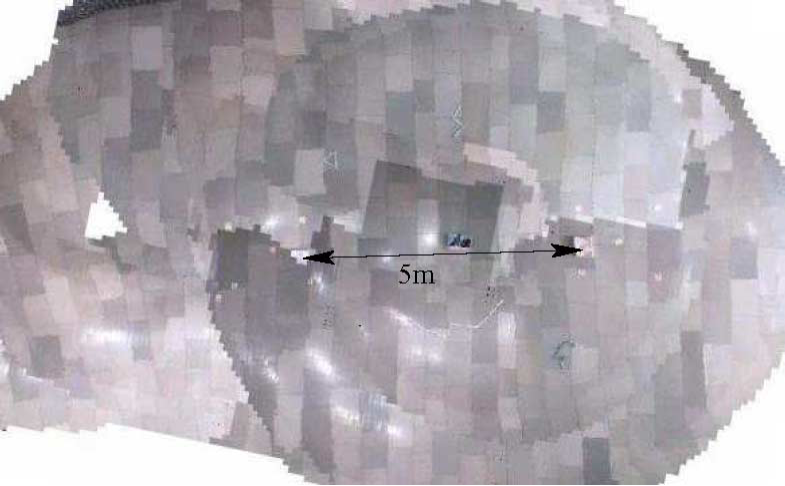
\includegraphics[height=3.5cm]{images/steder_blimp.png}}
    \hspace{1cm}
    \subfigure[Map constucted by a stereo camera platform. A sensor platform was mounted on a rod to simulate a freely floating vehicle.]{\label{steder_outdoor}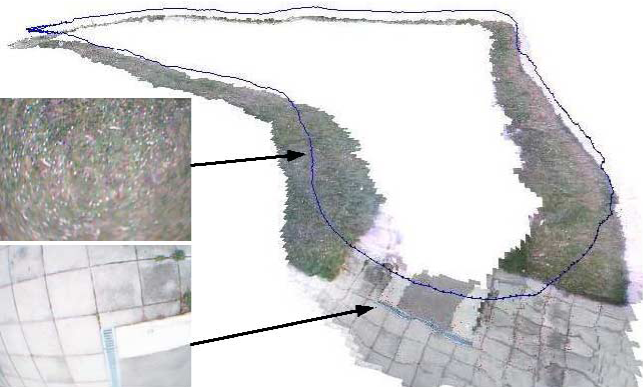
\includegraphics[height=3.5cm]{images/steder_outdoor.png}}
   
  \end{center}
  \caption{Visual maps obtained with the visual SLAM system presented in \cite{steder2008visual} (Courtesy Steder \textit{et al.} \cite{steder2008visual}).}
  \label{featureImg}
\end{figure}

Each node models a 6 degree of freedom camera pose.
The spatial constraints between two poses are computed from the camera images and the inertia measurements.
%The camera images are used to estimate the relative motion of the camera.
To do so, visual features are extracted from the images obtained from downlooking cameras.
Steder uses Speeded-Up Robust Features (SURF) \cite{Bay2008cviu} that are invariant with respect to rotation and scale.
By matching features in current image to the ones stored in the previous $n$ nodes, one can estimate the relative motion of the camera (\textit{visual odometry}).
The inertia sensor provides the roll and pitch angle of the camera.
This reduces the dimensionality of each pose that needs to be estimated from $\R^6$ to $\R^4$.
For each node, the observed features as well as their 3D positions relative to the node are stored.
The constraints between nodes are computed from the features associated with the nodes.

In the case of place revisiting, they compare the features of the current frame with all previous featured.
To speed up this potentially expensive operation, multiple filters are used.
First, only the features from robot poses that lie within Tipaldi's \cite{tipaldi2007approximate} confidence interval are used.
Second, only the best features from the current image are used (i.e., features with the lowest descriptor distance during visual odmetry).
Finally, a $k$-D tree is used to efficiently query for similar features, together with the best-bins-first technique proposed by Lowe \cite{lowe1999object}.

The camera pose is computed as following.
Using known camera calibration parameters, the positions of the features are projected on a normalized image plane.
Now, the altitude of the camera is computed by exploiting the similarity of triangles.
Once the altitude is known, the yaw of the camera is computed by projecting map features (from previous camera images) into the same normalized image plane.
When matching two features from the camera image against two features from the map, the yaw is the angle between the two  lines on this plane.
Finally, the feature positions from the camera image are projected into the map according to the known altitude and yaw angle.
The $x$ and $y$ coordinates are determined as the difference between the positions of the map features and the projections of the corresponding image points.

Both visual odometry and place revisiting return a set of correspondences, from which the the most likely camera transformation is computed.
First, these correspondences are ordered according to the Euclidean distance of their descriptor vectors, such that the best correspondences are used first.
The transformation $T_{c_a,c_b}$is determines for each correspondence pair.
This transformation is then evaluated based on the other features in both sets using a score function.
The score function calculates the relative displacement between the image features and the map features projected into the current camera image.
The solution with the highest score is returned as the assumption for the transformation.

Features correspondences between images are selected using a deterministic PROSAC \cite{chum2005matching} algorithm.
PROSAC takes into account a quality measure (e.g., distance between feature descriptors) of the correspondences during sampling, where RANSAC draws the samples uniformly.

This article describes how to estimate the motion of a vehicle and perform place revisiting using a feature map.
However, the article doesn't describe how the visual map is constructed (from poses and images) and visualized.
Furthermore, it lacks how an elevation map is constructed and how this elevation map can be used to improve the position estimates (e.g., elevation constraints).
A great disadvantage of the described method are the computational costs of the optimization method, which cannot be performed online (i.e. during flight). This reduces the number of practical applications.


\subsubsection{Online Mosaicking}
While Steder uses a Euclidean distance measure to compare the correspondences of the features in two images, Caballero \textit{et al.} \cite{caballero2009unmanned} indicate that this is a last resort.
They are able to make a robust estimation of the spatial relationship on different levels: homogeneous, affine and Euclidean.
The article addresses the problem for aerial vehicles with a single camera, like the AR.Drone.
%Geo-referenced mosaics can be sufficient as environment model for certain tasks.
A mosaic is built by aliging a set of images gathered to a common frame, while the aerial vehicle is moving.
A set of matches between two views can be used to estimate a homographic model for the apparent image motion.

\begin{figure}[htb]
\centering
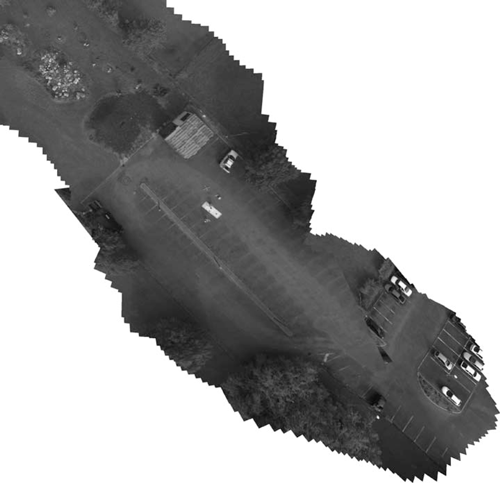
\includegraphics[width=6cm]{images/Caballero_map.png}
\caption{Mosaic constructed with a KARMA autonomous airship flying at $22\small{m}$ (Courtesy Caballero \textit{et al.} \cite{caballero2009unmanned}).}
\label{fig:Caballero_map}
\end{figure}


The homography that relates two given images is computed from sets of matched features.
Depending on the scene characteristics (e.g., the parallax effect and small overlap between images), the homography computation could become a hard problem. 
A classical solution to improve the results is to introduce additional constraints to reduce the number of degrees of freedom of the system of equations.
This is accomplished through a hierarchy of homographic models, in which the complexity of the model to be fitted is decreased whenever the system of equations is ill-constrained.
An estimation of this accuracy will be given by the covariance matrix of the computed parameters.

If most of the matches are tracked successfully, a \textit{complete homogeneous transformation} (8 degrees of freedom) is estimated.
Least median of squares (LMedS) is used for outlier rejection and a M-Estimator  \cite{zhang1997parameter} to compute the final result.
When the number of correspondences is too low, an \textit{affine transformation} (6 degrees of freedom) is estimated.
LMedS is not used, given the reduction in the number of matches.
Instead, a relaxed M-Estimator (soft penalization) is carried out to compute the model.
Only when the features in the image are really noisy a \textit{Euclidean transformation} (4 degrees of freedom) is estimated.
The model is computed using least-squares.
If the selected hierarchy level is not constrained enough (e.g., the M-Estimator diverges by reaches the maximum number of iterations), the algorithm decreases the model complexity.
Once the homography is computed, it is necessary to obtain a measure of the estimation accuracy.
Caballero uses a $9 \times 9$ covariance matrix of the homography matrix, which is explained in \cite{hartley2000multiple}.

The (ego-) motion of the vehicle is computed using the estimated homographies.
This method assumes that the terrain is approximately flat and that cameras are calibrated.
$H_{12}$ is the homography that relates the first and the second view of the planar scene.
Both projections can be related to the camera motion as:
\begin{equation}
H_{12} = AR_{12}(I - \frac{t_2n_i^T}{d_1})A^{-1}
\end{equation}
where $A$ is the camera calibration matrix, $t_2$ is the relative translation of the second view, $n_1$ is an unitary vector normal to the plane in the first camera coordinate frame, $d_1$ is the distance from the first camera to the plane and $R_{12}$ is the rotation matrix that transforms a vector in the first camera coordinate frame into a vector expressed in the second camera coordinate frame.
If the camera calibration matrix $A$ and the distance to the ground $d_1$ are known, it is possible to extract the motion of the vehicle.
Triggs \cite{triggs1998autocalibration} proposes a robust algorithm based on the singular value decomposition of the calibrated homography, defined by:
\begin{equation}
H_{12}^{u} = A^{-1} H_{12} A
\end{equation}

A classical static mosaic is not appropriate, as the uncertainties should be taken into account along the mosaicking process.
Therefore, the mosaic is augmented by including stochastic information, resulting in a set of images linked by stochastic relations.

The position of the image inside the mosaic is obtained by multiplying the current homography by all the previous homographies.
This estimation will drift along time, but can be compensated by building a mosaic.
By comparing the current image with images previously stored in the mosaic, loop-closures can be detected and used to eliminate the accumulated drift.
The crossover detection consists of finding one image whose Mahalanobis distance is within a certain empirical range.
Once an image is detected, a feature matching is used to compute the alignment between both images. 
\textit{In the general case, the task of matching images taken from very different viewpoints is difficult and computationally costly.}
For this reason, the image is warped to match the image from the mosaic, which simplifies the problem.
The computed homography is used to obtain the correct alignment.
Now, the relations among the most recent image and the corresponding image from the mosaic can be updated.

The relations between images are maintained and updated by using an Extended Kalman Filter.
The state vector including the mean and covariance of all images is defined as:
\begin{equation}
x^{-} = [x_1, x_2, ..., x_n]^T = [h_{01}, x_1 \cdot h_{12}, ..., x_{(n-1)n} \cdot h_{(n-1)n}]^T
\end{equation}
The correction obtained when a loop-closing is detected is employed to update the state.
All states affected by the correct are now update by the Extended Kalman Filter.

Similar to Steder's research, Caballero uses a probabilistic representation of the estimated poses.
Both approaches optimize the map after a loop-closure event is detected, but use different optimization methods.
Unfortunately, these optimization methods are computationally expensive and difficult to perform while flying.
Steder exploits the information from the inertia sensor to reduce the complexity of pose estimation, without decreasing the accuracy (degree of freedom) of the estimated pose.



\section{Airborne elevation mapping with an ultrasound sensor}
Multiple techniques have been presented that successfully employ an airborne radar sensor for building elevation maps (e.g., \cite{foessel2000radar, weiß2006airborne}).
Due to its large footprint, a radar sensor cannot be mounted on small UAVs.
Unlike a radar sensor, an ultrasound sensor can be carried by a small UAV.
This sensor provides feedback for altitude stabilization and obstacle detection.
According to my knowledge, no publication addresses the problem of elevation mapping using a single airborne ultrasound sensor.
However, the problem is addressed using advanced (e.g., multibeam) ultrasound sensor.

\subsubsection{Seafloor mapping}
Seafloor mapping is a research area for which ultrasound sensors have been used for building elevation maps. Some examples are \cite{johnson1996seafloor,strauss1999multibeam,zerr1996three,evans2002three}.
\cite{kenny2003overview} Gives and overview of seabed-mapping technologies.
Elevation mapping is essential for an autonomous underwater vehicle designed to navigate close to the seafloor.
The map is being used for obstacle avoidance, path planning and self-localization.

Given the limited range and applicability of visual imaging systems in the underwater environment,
sonar has been the preferred solution \cite{blondel1997handbook} for the observation of the seabed.
Most approaches use a side scan sonar system, that returns an image instead of a single distance measurements.
Side scan uses a sonar device that emits conical or fan-shaped pulses down toward the seafloor.
The intensity of the acoustic reflections from the seafloor of this beam is recorded in multiple transducers.
When stitched together along the direction of motion, these slices form an image of the sea bottom within the coverage of the beam.
Modern side scan devices offer high-resolution images of the seabed on which objects on the order of tens of cm may be detected at a range of up to 100 m.

\begin{figure}[htb]
\centering
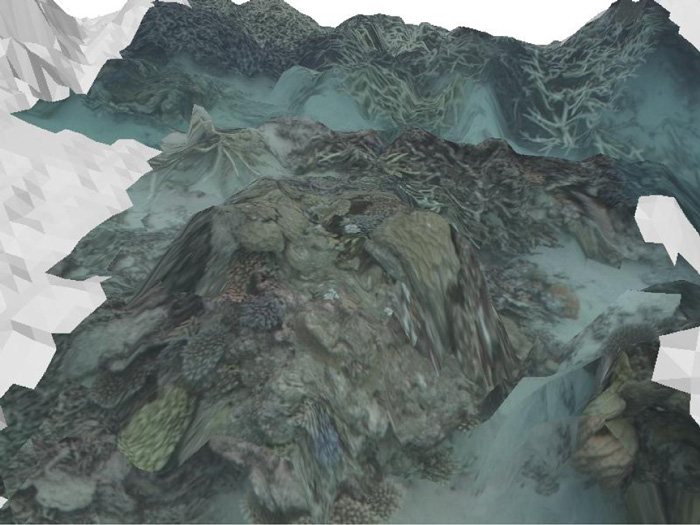
\includegraphics[width=7.5cm]{images/williams_seabed_map.jpg}
\caption{Seabed terrain model built by projecting the texture of the visual images onto a surface model generated by the sonar data.
The grey areas represent portions of the terrain only observed using the vehicle’s sonar. (Courtesy Williams and Mahon \cite{williams2004simultaneous}).}
\label{fig:williams_seabed_map}
\end{figure}

A particularly interesting application of sonar-based elevation mapping is presented in \cite{williams2004simultaneous}.
The article presents a SLAM system that uses information from the on-board sonar an vision system of an Unmanned Underwater Vehicle (UUV).
The system estimates the vehicle's motion and generates a model of the gross structure of the underlying reefs.
This work shows correspondences to the methods used in this thesis.
Unlike the AR.Drone, the pencil beam scanning sonar of the UUV returns high-resolution images instead of a single distance measurents.

In cases where a priori maps are not available, a mechanism must exist for building a map while simultaneously using that map for the purposes of localisation.
During motion, the vehicle builds a complete map of landmarks and uses these to provide continuous estimates of the vehicle location.
By tracking the relative position between the vehicle and identifiable features in the environment, both the position of the vehicle and the position of the features can be estimated simultaneously.
An Extended Kalman Filter (EKF) is used for stochastic estimation of the vehicle's position and map feature locations.
The state is represented by an augmented state vector $\hat{x}^{+}(t)$, consisting of $n_v$ states.
\begin{equation}
\hat{x}^+ = \left[ {
\begin{array}{c} \hat{x}_0^+ \\ \vdots \\ \hat{x}_{n_v}^+ \\  \end{array}
} \right]
\end{equation}
Each state $\hat{x}_t^+$ consists of a vehicle state $\hat{x}_v$ and the observed features $\hat{x}_{f, i}, i = 0, ..., n_f$, where $n_f$ is the number of features.
\begin{equation}
\hat{x}_t^+ = \left[ {
\begin{array}{c} \hat{x}_v \\ \hat{x}_{f, 0} \\ \vdots \\ \hat{x}_{f, n_f} \\  \end{array}
} \right]
\end{equation}
The covariance matrix for the state at time $t$ is defined as:
\begin{equation}
\textbf{P}^+_t = E[(x_t - \hat{x}^+_t)(x_t - \hat{x}^+_t)^T | \textbf{Z}^k]
\end{equation}
It was assumed that the roll and pitch of the vehicle were negligible, based on observations of the vehicle performance during in-water tests and results from the design of the vehicle.
The vehicle pose at time step $k$ is represented by
\begin{equation}
\hat{x}^+_v(t) = \left[ \begin{array}{cccc} \hat{x}^+_v(t) & \hat{y}^+_v(t) & \hat{z}^+_v(t) & \hat{\psi}^+_v(t) \end{array}\right]^T
\end{equation}
and the features states are represented by
\begin{equation}
\hat{x}^+_i(t) = \left[ \begin{array}{ccc} \hat{x}^+_i(t) & \hat{y}^+_i(t) & \hat{z}^+_v(t) \end{array}\right]^T
\end{equation}

Ultrasound and vision information can be combined to aid in the identification and classification of natural features present in the environment.
For maximum overlap of both sensors the ultrasound sensor is mounted directly above the high-resolution vision system.
The ultrasound sensor scans the sea floor directly below the vehicle and is used to generate
profiles of the surface.
The returns \textbf{received} by the ultrasound are then processed to identify the \textbf{principal returns} which are used to initialise new features in the SLAM map.
The observation of range $R$ and bearing $\theta$ are combined with the estimated value of the vehicle pose $\hat{x}_v(t)$ and the measured position
$\left[ \begin{array}{ccc} x_s & y_s & z_s \end{array}\right]^T$ of the sonar relative to the camera frame.
\begin{equation}
\left[ {
\begin{array}{c} \hat{x}_i \\ \hat{y}_i \\ \hat{z}_i \end{array}
} \right] =
\left[ {
\begin{array}{c}
	\hat{x}_v + x_s cos \hat{\psi}_v - (y_s + R cos \theta) sin \hat{\psi}_v \\
	\hat{y}_v + x_s sin \hat{\psi}_v + (y_s + R cos \theta) cos \hat{\psi}_v \\
	\hat{z} + z_s + R sin \theta
\end{array}
} \right]
\end{equation}

Once the ultrasound returns have been initialized, they are tracked using observations from the vision system.
When a new feature is initialised, the sonar footprint is projected into the visual frame of the camera.
The centre of this footprint is then used to identify a high contrast feature in the image within the area convered by the sonar.
These visual features are tracked from frame to frame using the Lucas and Kanade feature tracking technique \cite{lucas1998application}.
Observation of elevation $z_e$ and azimuth $z_a$ are provided to the SLAM algorithm.
The estimated elevation and azimuth (orientation) are computed using the current estimate of the vehicle pose and feature position:
\begin{equation}
\left[ {
\begin{array}{c} \hat{z}_e \\ \hat{z}_a \end{array}
} \right] =
\left[ {
\begin{array}{c}
	(\hat{x}_i - \hat{x}_v) cos \hat{\psi}_v + (\hat{y}_i - \hat{y}_v) sin \hat{\psi}_v \\
	-(\hat{x}_i - \hat{x}_v) sin \hat{\psi}_v + (\hat{y}_i - \hat{y}_v) cos \hat{\psi}_v
\end{array}
} \right]
\end{equation}
The difference between the actual observation received from the camera and the predicted observation is the innovation, which is used in computing the posterior state estimate.
The current implementation makes use of very simple features.
These features are sufficient for tracking puroposes, but are not applicable to detected loop-closures.


\section{Research using the AR.Drone}
Because the AR.Drone is a quite recent development, the number of studies based on this platform is limited.

\subsubsection{Autonomous corridor and staircase flights}

A recent publication is from Cornell University \cite{Bills2011icra}, where an AR.Drone is used to automatically navigate corridors and staircases based on visual clues.
Their method method first classifies the type of indoor environment (e.g., corridors, staircases, rooms and corners) then uses vision algorithms based on perspective cues to estimate the desired direction to fly.
This method require very little computational power and can be used by a controller directly without building a 3D model.

The type of environment is determined using two algorithms.
The first method uses GIST features \cite{oliva2001modeling} with a Support Vector Machine (SVM) learning algorithm for classification.
GIST features are well-suited for this task because they directly measure the global distribution of oriented line segments in an image, which takes advantage of the long lines found in indoor images.
The second method computes a confidence estimate from both the stair and corridor vision algorithms.
The confidence values are compared, and the highest is used to select the environment type.

When navigating corridors, vanishing points are used to locate the end of the corridor. 
First, the Canny edge detector is used to detected edges and a probabilistic Hough transform is used to find long lines.
The vanishing points (i.e., end of the corridor) are found by searching for the image region which has the highest density of pair-wise line intersections.
A probabilistic model with Gaussians is constructed to model the noise in the location of a vanishing point.
Staircases can be nagivated by finding the center of the staircase, so the AR.Drone can follow the staircase using its onboard intelligence (i.e., altitude stabilization).
Lines that represent the staircase are found by classifying the line segments as horizontal or vertical and looking for the largest horizontal-line cluster in the Hough transform space.
Once the cluster of horizontal lines is detected, the mean of the lines' endpoints is calculated to retrieve the desired direction.

\subsubsection{Map\&replay bearing-only navigation}
Krajn{\'\i}k et al \cite{krajník2010simple,faiglsurveillance,krajník2011ar} present a simple monocular navigation system based on the map\&replay technique.
For this technique, a robot is navigated by a human through an environment and creates a map of its environment.
After the map is created, the robot starts at the start position and repeats the learned path.
The method can navigate a robot along a given path while observing only one landmark at a time, making it more robust than other monocular approaches.

The authors simplify the problem by splitting the route in straight line segments (i.e., the robot travels in straight lines and rotates between segments).
%At first, the robot is tele-operated in the environment along straight line segments in the mapping phase.
For each segment a set of visual landmarks is remembered, consisting of salient features extracted from the frontal camera image.
Similar to Steder, the authors use Speeded-Up Robust Features (SURF) to detect and represent salient features.
When entering a segment, the robot is rotated to match the rotation during the mapping phase.
During the navigation along a segment, the robot establishes correspondences of the currently seen and previously mapped landmarks and computes differences in the expected and recognized positions for each such correspondence.
The robot steers in a direction that reduces those differences while moving straight at a constant speed until its odometry indicates that the current segment has been traversed.
The heading is determined by a simple histogram voting procedure.
This navigation method is provably stable for nondegenerate polygonal paths, since the heading corrections can suppress the position uncertainty originating from the dead reckoning.
%The distance traveled along a segment is estimated purely by dead reckoning.
%Due to the low precision of the IMU based distance estimation, the localization error is high.
%However, the localization error does not diverge and is kept within sufficient limits allowing the drone to autonomously navigate along the learned path.




\chapter{Platform: Parrot AR.Drone}
\label{chapter:platform}
A preliminary step is to find a suitable robot platform that enables both the development and testing of indoor Aerial SLAM methods.
A straightforward choice is to use a \textit{quadrotor helcopter}, commonly designed to be unmanned aerial vehicles (UAVs).
Their small size and extremely maneuverability allows both indoor and outdoor flight.
Furthermore, quadrotors don't require mechanical linkages to vary the rotor blade pitch angle, which simplifies the design.

Nowadays, small quadrotors with on-board stabilization can be bought off-the-shelf.
These quadrotors make it possible to shift the research from basic control of the platform towards intelligent applications.
The platform selected is the Parrot AR.Drone\footnote{\url{http://ardrone.parrot.com}} quadrotor helicopter.
The main advantages of this quadrotor are the robustness and affordable pricetag.
The AR.Drone is equipped with a front-camera and a down-looking camera that provide live video streaming.
Furthermore, the AR.Drone is equipped with an ultrasound sensor and an inertial unit that measures pitch, roll, yaw and accelerations along all axes.
The vehicle is controlled by sending commands over a Wi-Fi connection.

In this chapter, the AR.Drone is evaluated as a robotic platform.
The flight control of a quadrotor is described and the AR.Drone's hardware is listed.
The intelligence onboard of the vehicle is described.
Moreover, the open Application Programming Interface (API) is examined.



% Quadrotor flight control
\section{Quadrotor flight control}
% http://www.stanford.edu/~haomiao/papers/ICRA09AeroEffects.pdf
% http://www2.engr.arizona.edu/~sprinkjm/research/c2wt/uploads/Main/QuadrotorDynamicsGNC.pdf
The mechanical structure of a quadrotor consists of four rotors attached to a body frame (see Figure \ref{fig:QuadRotorBody}).
Each pair of opposite rotors (pair ${1, 3}$ and pair ${2, 4}$) is turning the same direction.
One pair is turning clockwise and the other counter-clockwise.
Each rotor produces both a thrust $T$ and torque $\tau$ about its center of rotation, as well as a drag force $D_b$ opposite to the vehicle's direction of flight.
Thrust $T$ is a force that is generated by expelling or accelerating mass in one direction.
The accelerated mass will cause a force of equal magnitude but opposite direction on that system.
Torque $\tau$ is the tendency of a force to rotate an object about an axis.
Drag $D_b$ is the force that opposes the motion of an aircraft through the air.
This force depend on velocity of the vehicle and deaccelerates the vehicle if insufficient thrust is generated.
Together the motors should generate sufficient vertical thrust to stay airborne, which is indicated by the gravity force $mg$ in the direction $e_D$.

% TODO: diagram of roll, pitch, yaw

\begin{figure}[htb]
\centering
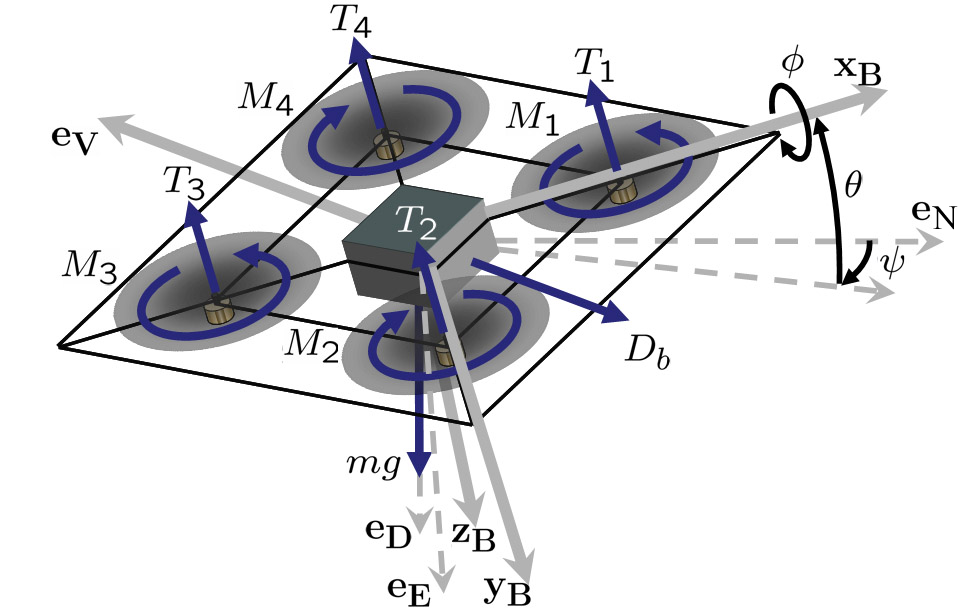
\includegraphics[width=7cm]{images/QuadRotorBody.png}
\caption{Free body diagram of a quadrotor helicopter 
(Courtesy Hoffman \textit{et al.} \cite{Hoffmann2007}). Note that a right-handed orthogonal coordinate system is used with the $z$-axis pointing down. Each of the 4 motors has a thrust $T_i$ and momentum $M_i$. Together the motors should generate sufficient vertical thrust to stay airborne, which is indicated by the gravity force $mg$ in the direction $e_D$. Differential thrust between the motors can provide roll $\phi$ and pitch $\theta$ torques, which lead to an angle of attack $\alpha$. This can result in fast movements of the helicopter (e.g. in the horizontal plane) in the direction $e_V$ which a resulting drag force $D_b$. }
\label{fig:QuadRotorBody}
\end{figure}

For movements, the quadrotor relies solely on differential torque and thrust.
If all rotors are spinning at the same angular velocity, the differential torque is zero, resulting in no angular acceleration about the yaw axis.
Varying the angular velocity of each rotor pair yields angular acceleration about the yaw axis.
If the total thrust is kept constant, the vertical velocity remains unchanged.
A vertical movement is achieved by increasing or decreasing the thrust from each motor by the same amount, so that total thrust changes but differential torque on the body remains zero. 
A horizontal movement is achieved by maintaining a non-zero pitch $\theta$ or roll angle $\phi$.
Angular accelerations about the pitch and roll axes can be caused separately.
Each pair of blades rotating in the same direction controls one axis, either roll or pitch.
Increasing thrust for one rotor while decreasing thrust for the other will maintain the torque balance needed for yaw stability and induce a differentie torque about the roll or pitch axes. 

\begin{comment}
\begin{figure}[htb]
\centering
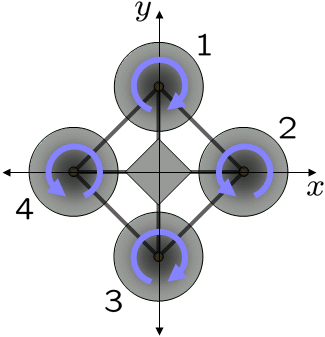
\includegraphics[width=7cm]{images/Quadrotor_yaw_torque.png}
\caption{Schematic of reaction torques on each motor of a quadrotor helicopter. Rotors 1 and 3 spin in one direction, while rotors 2 and 4 spin in the opposite direction, yielding opposing torques for control.}
\label{fig:QuadRotorRotors}
\end{figure}
\end{comment}

% Hardware
\section{Hardware}
The AR.Drone is remote-controlled consumer quadrotor helicoptor developed by Parrot SA\footnote{\url{www.parrot.com}}.
The body is made of carbon fiber tube structure and high resistance 
%PA66
plastic.
A protection hull is made of Polypropylene Foaming Material.
This hull provides protection during indoor flights.
The propellors are powered by four brushless motors (35,000 rpm, power: 15W).
Energy is provided by a Lithium polymer battery with a capacity of 1000 mAh, which allows a flight time of approximately 10 minutes.

The AR.Drone carries an internal computer with an 468MHz ARM9-processor and 128MB of RAM, running a custom Linux operating system.
A mini-USB connector is included for software flashing purposes and to allow add-ons to be plugged
An integrated 802.11g wireless card provides network connectivity with an external device that controls the vehicle.
No remote-control is provided. Instead, a regular wifi-enabled device can be used to control the AR.Drone.
It was initially designed for the Apple platforms (e.g., iPhone, iPod and iPad) and became available on other platforms in the last few months.
It is also possible to control the AR.Drone from a Linux or Windows PC with the software designed for application developers.



% Sensors
\subsection{Sensors}
The AR.Drone has different types of sensors.
These sensors are used for automatic stabilization.
In addition, a front camera is present to provide the user visual feedback from the vehicle.


\subsubsection{Inertial measurement unit}
The AR.Drone features an 6 degrees of freedom (DOF) inertial measurement unit.
It provides the software with pitch, roll and yaw measurements.
These measurements are used for automatic pitch, roll and yaw stabilization and assisted tilting control.
The measurement unit is a \textit{micro electro-mechanical system} (MEMS) and contains
a 3 axis accelerometer, a 2 axis gyrometer and a 1 axis yaw precision gyrometer.

The \textbf{accelerometer} is a BMA150\footnote{\url{http://www.bosch-sensortec.com/content/language1/downloads/BMA150_DataSheet_Rev.1.5_30May2008.pdf}} made by Bosch Sensortec.
%It provides three sensitivity ranges (i.e., maximum g-force it can report): $\pm 2g / \pm 4g / \pm 8g$.
An accelerometer outputs g-forces (acceleration relative to free-fall) as a quantity of acceleration.
It is based on the phenomenon that the (observed) weight of a mass changes during acceleration.
Typical MEMS accelerometer is composed of movable \textit{proof mass} with plates that is attached through a mechanical suspension system to a reference frame.
Movable plates and fixed outer plates represent capacitors. The deflection of proof mass is measured using the capacitance difference.
The accelerometer has three perpendicular axes. Each axis can only measure acceleration in the direction of the axis.
%The tiny micro-structures can only measure force in a single direction, or axis of acceleration.
%This means with a single axis measured, you can only know the force in either the X, Y, or Z directions.
An accelerometer at rest relative to the Earth's surface will indicate approximately 1 g upwards, because any point on the Earth's surface is accelerating upwards relative to the local inertial frame.
To obtain the acceleration due to motion with respect to the Earth, this gravity offset must be subtracted and corrections for effects caused by the Earth's rotation relative to the inertial frame.
Since the accelerometer can measure gravity, it can be used as a tilt sensor.

The AR.Drone has a 2 axis \textbf{gyrometer} and a 1 axis yaw precision gyrometer.
The gyrometer measures angular velocity in degrees per second, based on the principles of angular momentum.
In order to estimate the absolute angle $\theta$, the angular velocity signal $\Omega$ needs to be integrated with respect to time.
A major problem with this method is that bias errors in the angular velocity signal will cause the integrated angle value to drift over time, since all gyroscopes have at least a small amount of bias error in their angular rate signal.

Regular gyroscopes use a spinning wheel.
However, a small device like the AR.Drone cant afford to have a spinning wheel.
Instead, a tiny MEMS gyroscope is used. 
%In a MEMS gyroscope, two proof masses vibrate in plane at certain frequency.
It comprises of a plate, called the \textit{proof mass}, that vibrates (oscillates).
%when a drive signal is applied to set of drive capacitor plates.
When the vehicle rotates, the proof mass gets displaced in the X, Y, and Z directions by Coriolis forces.
A processor senses the proof mass’ displacement through capacitor plates located underneath the proof mass, as well as finger capacitors at the edges of the package.
The AR.Drone uses a IDG-500 Dual-Axis\footnote{\url{http://www.sparkfun.com/datasheets/Components/SMD/Datasheet_IDG500.pdf}} gyroscope for the X and Y axis of the drone.
The IDG-500 gyro has two separate outputs per axis for higher speed motions (range: $500^{\circ}/s$, sensitivity: $2.0mV/^{\circ}/s$) and lower-speed precise movements (range: $110^{\circ}/s$, sensitivity: $9.1mV/^{\circ}/s$).
The yaw orientation is measured using a high precision gyrometer: Epson Toyocom XV-3500CB\footnote{\url{http://www.eea.epson.com/portal/pls/portal/docs/1/424992.PDF}}.
%This sensor has a range of $100^{\circ}/s$
%Vibrating structure gyroscopes are simpler and cheaper than conventional rotating gyroscopes of similar accuracy
%The output is a rate of rotation about the X and Y axis.


\subsubsection{Ultrasound altimeter}
An ultrasound sensor provides altitude measures for automatic altitude stabilization and assisted vertical speed control.
The ultrasound sensor is attached on the bottom of the AR.Drone and points downwards in order to measure the distance to the floor.
A packet of ultrasonic soundwaves is transmitted towards the floor, which reflects the sound back to the sensor.
The system then measures the time $t$ for the echo to return to the sensor and computes the distance $d$ to the target using the speed of sound, using:
\begin{equation}
d = \frac{c \times t}{2}
\end{equation}
where $c \approx 343\small{m/s}$ is the speed of sound in air.

Altrasound range measurements suffer from some fundamental drawbacks which limit the usefulness.
These drawbacks are inherent to the principle of an ultrasonic sensor and their commonly used wavelengths.
\cite{borenstein1988obstacle} Describes some of these drawbacks in the context of obstacle avoidance.
A limitation is the small range in which the sensor is able to operate.
The ultrasound sensor in the AR.Drone has a effective range of approximately $20\small{cm}$ to $6\small{m}$.
%The minimum range is approximately $20\small{cm}$, meaning that the AR.Drone is \textit{unable to determine its altitude} when flying close to the floor.
Another limitation is that the ultrasound sensor is unable to obtain precise directional information about objects.
Sound progragates in a cone-like manner, where opening angles are commonly between 20 to 40 degrees.
Due to this property, the sensor acquires entire regions of constant depth instead of discrete depth points.
So, the ultrasound sensor can only tell there is an object at the measured distance somewhere within the measured cone.

Another limitation is the influence of the surface's orientation on the sensor's performance.
When the ultrasoundwave is emitted toward a parallel surface of an obstacle, most of the sound energy is reflected perpendicular to the surface and will be detected by the sensor.
However, if the surface of the obstacle is tilted relative to the sensor, then only an undetectably small amount of energy will be reflected toward the sensor.
Also, the acoustic properties of the material in range have direct impact on the sensor's performance (e.g., foam can acoustically absorb the soundwaves).
A final limition is the limited operating frequency.
Before a soundwave can be emitted, the previously emitted soundwave has to be detected by the sensor.
This reduces the minimal operating speed of the AR.Drone's ultrasound sensor to $300 / (2 \times 6) = 25\small{Hz}$.

\begin{center}
\line(1,0){250}
\end{center}
\color{mediumgray}
\small

The opening angle of the AR.Drone's ultrasound sensor is not documented.
A small experiment has been performed to determine the opening angle.

The AR.Drone was positioned at a fixed altitude of $79\small{cm}$ above a flat floor.
No obstacle was in range of the ultrasound sensor to make sure the measured altitude is the actual altitude of the AR.Drone.
The altitude measured by the ultrasound sensor was $75.2\small{cm}$, which equals an acceptable error of $3.8\small{cm}$.
The AR.Drone's bottom camera was used to mark a point on the floor that is exactly below the center of the AR.Drone.
This point is equal to the center of ultrasound cone.
In order to measure the opening angle, floating objects were moved from outside the cone towards the cone.
The objects require a certain distance from the floor to achieve a distance short than the shortest distance between the sonar and the floor.
The minimal altitude of an object when assuming a maximum opening angle of 40 degrees is:
\begin{equation}
a = 79\small{cm} - (cos(40\deg) \times 79\small{cm}) = 18.48\small{cm}
\end{equation}
Fluctuations in the altitude measurements indicate that the object is entering the cone.
The horizontal distance $d$ between the object and cone center (marked point) is the width of the cone and $h = 79\small{cm} - a$ is the height of the cone.
The angle $\alpha$ of the cone can be recovered with:
\begin{equation}
\alpha = tan^{-1}(d / h)
\end{equation}

The experiment was repeated 10 times with different objects.
The average opening angle is $25.03^{\circ}$ with a standard deviation of $1.45^{\circ}$.
\normalsize
\normalcolor


\begin{center}
\line(1,0){250}
\end{center}
\color{mediumgray}
\small

During flight, the AR.Drone can take a broad range of angles (the default maximum angle of attack is $12^{\circ}$).
The floor is not always perpendicular to the orientation of the ultrasound sensor, which may influence the altitude measurements.
A small experiment was performed to measure the effect of the AR.Drone's angle of attack $\alpha$ and the error $\epsilon$ of the measured altitude.

This experiment was performed above a flat floor.
The angle of attack $\alpha$ was changed slowly while keeping the AR.Drone at a fixed altitude.
A relation between the angle $\alpha$ and measured altitude was observed.
The following (first degree) polynomial fit describes the relation between the angle $\alpha$ and error $\epsilon$ of the measured altitude:
\begin{equation}
\epsilon = 0.2214 \times \alpha \hspace{0.2cm} \small{cm}
\end{equation}
\normalsize
\normalcolor



\subsubsection{Camera's}
The AR.Drone is equipped with two CMOS camera's: a front camera and a bottom camera.
Both camera's support live video streaming at 15 frames per second.

The front camera has a resolution of $640 \times 480$ pixels (VGA) and a wide $93^{\circ}$ field of view.
This front camera is used to automatically detect other drones during multiplayer games or to provide video feedback on a screen (e.g., smartphone).
The bottom camera has a resolution of $176 \times 144$ pixels (QCIF) and a $60^{\circ}$ field of view.
The video frequency of this camera is 60 frames per second to reduce motion blur and improve the applicability of intelligent algorithms.
Despite the high frequency, the frames are streamed at 15 frames per second.

\textit{front + bottom camera sample}

The bottom camera plays a central role in the AR.Drone's onboard intelligence.
It is used for horizontal / vertical stabilization (i.e., automatic hovering and trimming) and to estimated the velocity of the drone.
More details about the onboard intelligence can be found in Section \ref{sec:platform_onboard_intelligence}.



% Onboard intelligence
\section{Onboard intelligence}
\label{sec:platform_onboard_intelligence}
Usually quadrotor remote controls feature levers and trims for controlling pitch, roll, yaw and throttle.
It generally takes hours of practice to safely perform basic manoeuvres like take-off, trimming, hovering with constant altitude, and landing.
Thanks to the onboard computer and sensors, take-off, hovering, trimming and landing are now completely automatic and all manoeuvres are completely assisted.

Because the quadrotor system is unstable, feedback from the sensors to the control system is needed.
This raises the issue of state estimation.
The vehicle control system must be robust to the various disturbances that can be encountered in practice.
Redundancy in the state estimation is the solution in this case.
The AR.Drone has multiple methods to compute estimated states.
However, the onboard software (firmware) is closed source and not documented by the manufacturer.
In august, the manufacturer's academic partner \textit{MINES ParisTech for navigation and control design}, published an article \cite{bristeau2011navigation} which described the navigation and control technology inside the AR.Drone.



\subsection{Sensor calibration}
The AR.Drone uses low-cost sensors, which introduce issues like bias, misalignment angles, and scale factors.
These errors are not negligible and differ between AR.Drones.
For this reason, a manual board calibration is performed at the \textit{factory}.
This calibration process computes the unknown parameters using a least-square minimization method:
\begin{equation}
Y_m = AY_v + B
\end{equation}
where $Y_m$ is the measurement and $Y_v$ the true value of the sensed variable.

Not all errors are compensated during the factory calibration.
The AR.Drone's navigation board is mounted on damping foam.
To further compensate the misaligment, \textit{onboard calibration is performed}.
This is done by considering that the mean acceleration of the UAV must be equal to zero on a stationary flight.
A least-squares minimization method is used to determine the micro-rotation.
After each landing, this onboard calibration is automatically performed to compensate for the misalignment due to the displacement of the damping foam during the stopping shock.

After inertial sensors calibration, sensors are used inside a complementary filter to estimate the attitude and de-bias the gyroscopes.
The de-biased gyroscopes are used for vision velocity information combined with the velocity and altitude estimates from a ver- tical dynamics observer
The velocity from the computer vision algorithm is used to de-bias the accelerometers, the estimated bias is used to increase the accuracy of the attitude estimation algorithm.
Finally, the de-biased accelerometer gives a precise body velocity from an aerodynamics model.


\subsection{State estimation}
To address the problem of state estimation, the AR.Drone is equipped with embedded sensors that are described in the previous section.
When combining the sensor measurements in data fusion algorithms, relatively good state estimates are obtained.
Multiple techniques form a tightly integrated vision and inertial navigation filter that can be summarized as follows.
After inertial sensors calibration, sensors are used inside a complementary filter to estimate the attitude and de-bias the gyroscopes.
The de-biased gyroscopes are used for vision-based velocity information provided by the vertical camera.
The vision-based velocity is used to de-bias the accelerometers. This estimated accelerometer bias is used to increase the accuracy of the attitude estimation algorithm.
Eventually, the de-biased accelerometer gives a precise body velocity from an aerodynamics model.
Below, some techniques are described is more detail.

\subsubsection{Vision-based velocity}
The images provided by the vertical camera are used to estimate the 3D velocity of the vehicle (vision-based velocity).
According to \cite{bristeau2011navigation}, two complementary algorithms are available.
Depending on the scene content or the expected quality of their results, one is preferred to the other.

The first algorithm is a multi-resolution scheme.
The methodolog described in \cite{lukas1981iterative}.
It computes the optical flow over the whole picture range using a kernel to smooth spatial and temporal derivatives.
Attitude changes between two images are ignored during the first resolution refinement step.
The error is finally efficiently canceled in most cases by subtracting the displacement of the optical center induced by the attitude change alone.
The second algorithm estimates the displacement of several interesting image points (features).
For this, FAST image features are used.
An iteratively weighted least-squares minimization procedure is used to recover the displacements.
The IRLS estimation \cite{michaelsen2004pose} is carried out by assuming the depth of the scene is uniform.
This optical flow based method is used by default.
When the scene is deemed suitable for the corner detector and the speed is low, the system switches to the second algorithm for increased accuracy.

The inertial sensors are used to compensate for the small rotation between consecutive camera frames.
This is a significant help for the determination of the optical flow in the vision algorithm.
A specific linear data fusion algorithm combining sonar and accelerometer information is implemented to give accurate vertical velocity and position estimates above the obstacle.

\subsubsection{Aerodynamics model}
Unfortunately, the vision-based velocity is noisy and relatively slowly updated compared to the vehicle dynamics.
The estimated velocity is improved with the help of an aerodynamics model.
The accelerometers and gyroscopes are used together as inputs in the motion dynamics to estimate the attitude and velocities.
When the aerodynamics velocity and the vision velocity are simultaneously available, the accelerometer bias is estimated and vision-based velocity is filtered.
Alternatively, when vision-based velocity is unavailable, only the aerodynamics estimate is used with the last updated value of the bias.

The dynamic behavior of a quadrotor is quite complex.
In particular, the aerodynamics of the propellers and the motion of the rigid frame can interfere to produce a coupled dynamical model.
This model is beyond the scope of this thesis.
In summary, linear drag term exists from the interaction between the rigid body and the rotors and this term is reinforced by tilt phenomenon which changes a lift force component in drag.
These induced-drag effects are non negligible and they yield interesting information on the velocity of the system.
The induced forces are directly measured by the accelerometers, and through the model, can be used to reliably estimate the velocities of the vehicle.



\subsection{Controls}
The AR.Drone performs actions based on the estimated state and the input from the pilot.
A pilot controls the linear and lateral velocity with an input signal $s$ that specifies the pitch of the drone as a factor (between 0 and 1) of the maximum absolute tilt $\theta_{max}$.
The altitude is controlled with an input signal that specifies the derised vertical speed as a factor (between 0 and 1) of the maximum vertical velocity $v_{max}$.
A finite state machine is used to handle different modes of the vehicle (e.g., flight, hovering, take off and landing).

The control is realized by two nested loops, the \textit{Attitude Control Loop} and the \textit{Angular Rate Control Loop}.
The Attitude Control Loop computes an angular rate from the difference between the estimated attitude and the desired attitude (which is based on the velocity requested by the pilot).
The angular rate is tracked with a Proportional Integral (PI) controller.
The Angular Rate Control Loop controls the motors with simple proportional controllers.
When no user input is given, the AR.Drone goes in hovering mode, where the attitude and velocity are stabilized to zero.
Transition from flight mode to hovering mode is realized with a motion planning technique, designed to obtain zero speed and zero attitude in short time and without overshooting.
For this, a feed-forward control uses inversion of the governing dynamics.
The hovering mode is maintained by the Hovering Control Loop, which consists of a PI controller on the speed estimate.

The Attitude Control Loop is also responsible for altitude stabilization (i.e., maintaining a fixed distance between the floor and vehicle).
For this, feedback from the ultrasound sensor is used.
When an obstacle is in range of the ultrasound sensor, the measured altitude decreases.
The AR.Drone responds by increasing its absolute altitude to maintain a fixed measured altitude.
Consequently, the AR.Drone decreases its absolute altitude when the obstacle is out of range.
However, this behavior was not always observed during experiments.
For example, when a floating object ($1\small{m}$ above the floor) become in range of the ultrasound sensor.
In these cases, the raw ultrasound measurements show a sudden large change, while the filtered altitude measurements show a small change (Figure X).
Now, AR.Drone does not change its absolute altitude and remains at the same absolute altitude.
Based on this observation, we suspect that the altitude stabilization is based on a filtered derivative \small{(raw measurements should cause convergence to the actual measurements over time)} of the raw ultrasound measurements.
The filter minimizes the impact of sudden changes that occur for a short period.

[plot]

Similar to altitude stabilization, the ultrasound sensor is used for take-off and landing.
When a take-off command is issued, the engines are started automatically and the AR.Drone increases its altitude until a pre-determined altitude is reached (which is $50\small{cm}$ by default). When this altitude is reached, the vehicle switched to hovering mode.
During the take-off procedure, the AR.Drone is likely to generate some (random) horizontal movements.
These movements are often not observed by the AR.Drone's internal state estimation, probably due to the bad lightning condition for the vision-based algorithms.
In case of a landing command, the AR.Drone decreases its altitude until it has landed on the floor. The vertical velocity is decreased when the drone comes near the floor to prevent a heavy shock.
The engines are stopped automatically stopped.

\textit{Funny observation: sticking tape on the ultrasound sensor results in infinite take-off and landing (e.g., vehicle keeps increasing or decreasing altitude).}


% Open application programming interface
\section{Open Application Programming Interface}
\label{sec:API}
The AR.Drone API\footnote{\url{https://projects.ardrone.org}} (Application Programming Interface) is the reference project for developing applications for the AR.Drone.
It includes SDK source code (written in C), multiplatform examples and documentation.
The API does not include software that is embedded on the AR.Drone.

Communication with the AR.Drone is done through four main \textit{communication services}, which are implemented in the SDK.
\begin{enumerate}
\item Controlling and configuring the drone is done by sending \textit{AT commands} on regular basis;
\item Information about the drone (e.g., status, attitude, speed) is called \textit{navdata}.
The navdata also includes filtered and raw sensor measurements.
This information is sent by the drone to its client at a frequency of approximately 30 (demo mode) or 200 times per second;
\item A video stream is sent by the AR.Drone to the client device.
Images from this video stream are decoded using the codecs included in this SDK.
\item Critical data is communicated over channel called the \textit{control port}.
This is a TCP connection to provide reliable communication.
It is used to retrieve configuration data, and to acknowledge important information such as the sending of configuration information.
\end{enumerate}

\begin{figure}[htb]
\centering
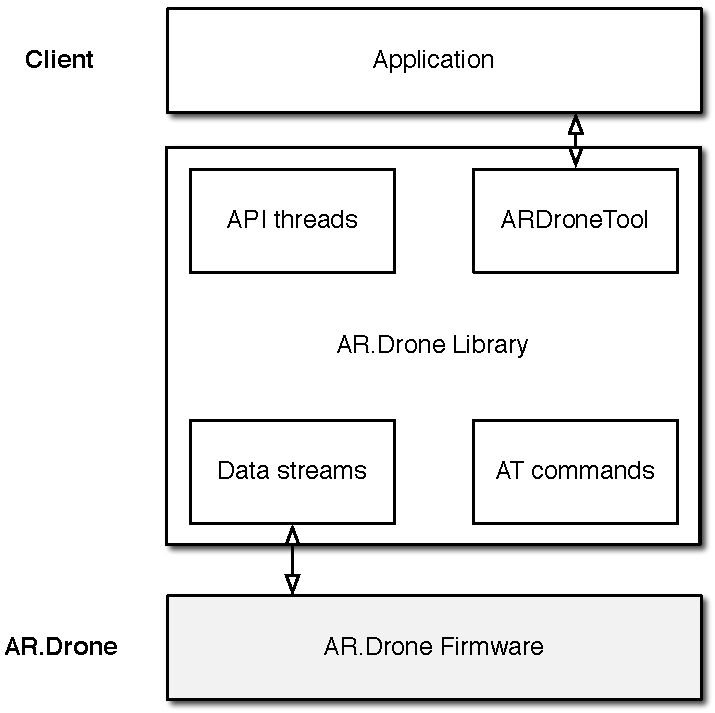
\includegraphics[height=8cm]{images/platform_ardroneapi.pdf}
\caption{Layered architecture of a client application built upon the AR.Drone SDK.}
\label{fig:platform-ardroneapi}
\end{figure}

The \textit{AR.Drone Library} is part of the SDK and provides high level APIs to access the drone.
Its conent can be summarized as following:
\begin{itemize}
\item \textit{SOFT}, includes header files describing the communication structures;
	\begin{itemize}
		\item \textit{ARDroneTool} a set of tools to easily manage the drone, e.g., communication initialization, input-device management, high-level drone control functions and navdata receiving and decoding system;
	\end{itemize}
\item \textit{VPSDK}, a set of general purpose libraries: video processing pieces, multiplatform wrappers for system-level functions, multiplatform wrappers for communication functions and helpers to manage video pipelines and threads;
\item \textit{VLIB}, the video processing library. It contains the functions to receive and decode the video stream.
\end{itemize}

Unfortunately, the AR.Drone API has some drawbacks.
The API was mainly developed for the iPhone application.
Support for other platforms (e.g., Linux and Windows) was added in an early release and not updated for a while.
In order to make recent versions of the API working under Windows, a significant amount of fixes is required.
Another drawback is the bulkiness.
The API consists of many files and lines of undocumented code.
This makes it difficult to comprehend what's happening inside the code.

For these reasons, custom software libraries have been released by developers.
ARDrone-Control-.NET\footnote{\url{https://github.com/shtejv/ARDrone-Control-.NET}} provides a .Net SDK for Windows.
Another developer has written a MeeGo\footnote{\url{http://www.developer.nokia.com/Community/Blogs/blog/kate-alholas-forum-nokia-blog/2010/12/23/ar-drone-with-meego}} application to control the AR.Drone on Nokia devices. The AR.Drone logic is written in C++.
Another interesting project is an Urbi driver\footnote{\url{http://www.psykokwak.com/blog/}} in order to control and program the ARDrone from the Urbi platform.
Urbi is an open-source software platform to control robots or complex systems in general. The goal of Urbi is to help making robots compatible, and simplify the process of writing programs and behaviors for those robots. 



\chapter{Development environment}
\label{chapter:development-environment}
As indicated by Michael et al \cite{Michael2010ra}, an accurate simulation of a quadrotor is a valuable asset, which allows safe and efficient development of control algorithms. Additionally, it gives direct access to ground truth values and allows to design repeatable experiments.

This chapter proceeds as follows.
First, the AR.Drone simulation model is presented.
This simulation model consists of a motion model, visual model and sensor model.
In order to validate the methods presented in Section \ref{chapter:visual-slam} on both the real and the simulated AR.Drone, an abstraction layer is required.
This abstraction layer is part of the framework proposed in Section \ref{sec:proposed-framework}.

	\section{Simulation model}
The simulation environment selected is USARSim \cite{Balakirsky2009iros,carpin2007usarsim}, which is based on the Unreal Tournament game engine\footnote{\url{http://www.unrealengine.com}}.
It allows physical realistic simulations and includes a versatile environment editor.

		\subsection{USARSim simulation environment}
USARSim is an open source high fidelity robot simulator that can be used both for research and education.
It builds upon the Unreal Tournament game engine, a widely used and affordable state of the art commercial game engine.
The engine provides realistic rendering and physical simulation.
USARSim in itself is a set of models and a hierarchy of classes defining the simulation of robots, sensors and actuators.
The simulator is highly configurable and extendible: users can easily add new sensors or robots.
The level of effort devoted to validation has been a distinguishing feature of USARSim.
Each of its major constituents (e.g., robot kinematics, interaction with the environment, sensors, and camera video) have been subjected to ongoing validation testing \cite{formsma2011realistic,carpin2006high,wang2005validating,carpin2007bridging,carpin2006quantitative}.

USARSim was originally developed aiming to Urban Search And Rescue simulation.
The RoboCup Rescue league is part of the RoboCup\footnote{\url{http://www.robocup.org}} initiative.
This league aims at the development of robotics artifacts that could effectively help human rescuers in the aftermath of disasters like earthquakes, terroristic attacks, and other extreme situations.
In addition to a Rescue league with real robots, the Virtual Robots Competition was started, which uses USARSim as simulation environment.
%The first tournament took place during RoboCup 2006, with the participation of eight teams from four continents.

Another key feature of USARSim is the \textit{UnrealEd}\footnote{\url{http://nl.wikipedia.org/wiki/UnrealEd}} versatile environment editor.
The editor is part of Unreal Tournament and can be used to create an modify virtual environments.
It includes geometrical modeling tools which can import and export models compatible with most commercially available modeling software packages.
The details needed for an experiment or competition can be easily added (e.g., roads, fire).



		\subsection{Motion model}
The AR.Drone is a stabilized system (Figure \ref{fig:QuadRotorBody}). When no control signals are given the quadrotor hovers on the same location, which is accomplished by a feedback loop which uses the ultrasound sensor (for altitude) and the bottom camera (for horizontal position). The simulation makes use of this assumption. When no control signal is given, the AR.Drone stays at the same location.
When a control signal for a linear (forward/backward) or lateral (sideward) velocity is given, it calculates the force needed to reach that velocity (and assuming that the drag force $D_b$ increases linearly with the velocity). When the control signal stops, the drag force $D_b$ slows the quadrotor down until it hovers again.
The USARSim quadrotor model uses the Karma physics engine (part of the Unreal Engine \cite{Carpin2006}) to simulate the force and torque acting on the aircraft. Yet, only the overall thrust is calculated, the differential thrust is not used.
When moving in the horizontal plane, a real quadrotor changes its angle of attack (which is the defined as the angle between direction of motion $e_V$ and the body frame $e_N$ \cite{Yechout2003}). 
The Karma physics engine does not need this angle to calculate the resulting horizontal movement. Yet, this angle of attack has direct consequences for the viewing directions of the sensors, so the roll and the pitch should be adjusted in correspondence with horizontal movements. The active control of the AR.Drone is incorporated in the value of the dragforce $D_b$.

Control signals for vertical and rotational movements (around the z-axis) are calculated in the same manner. For vertical movements not only the drag force $D_b$ is taken into account. In this case also the gravitational force $mg$ is included in the equation. Rotations around the z-axis stop quite quickly when no control signal is given. For this rotational movement a strong drag force $D_r = 20 \times D_b$ is used to model the additional inertia. 

The principal elements of inertia are calculated correspondingly to $(0.0241, 0.0232, 0.0451)\small{kg\cdot m^2}$, assuming a homogeneous distribution of the mass.

The result is a simulation model which maneuvers in a way similar to the actual AR.Drone, as demonstrated in Section~\ref{sec:simulation_results}.


		\subsection{Sensor model}
The USARSim simulator has a set of configurable sensors, which include all the sensors from the AR.Drone.
Each mounted sensor is triggered at fixed time intervals (every $200\small{ms}$ by default).
The AR.Drone's time interval is reduced to $5\small{ms}$, producing up to 200 sensor measurements per second.

The ultrasound sensor emits a number of traces, which in combination form a cone.
First the sensor sends out one trace in the direction of its orientation remembering the measured range.
Then it does several conical measurements and calculates the minimal measured distance.
If the angle between a trace and the surface normal is smaller than angle $\alpha_{maxIncidence}$ the measurement is ignored.

\begin{figure}[htb!]
\centering
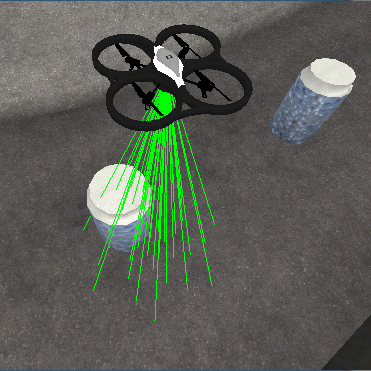
\includegraphics[width=6cm]{images/usarsim_sonar_beams.png}
\caption{The ultrasound sensor is modeled by emitting a number of traces, which in combination form a cone.} 
\label{fig:3Dmodel}
\end{figure}


The acceleration sensor computes the body accelerations using the AR.Drone's velocity:
\begin{equation}
a_{t} = (v_{t} - v_{t-\Delta t}) / \Delta t
\end{equation}
where $\Delta t$ is the time between measurements and $v$ is the velocity of the AR.Drone. The velocity of an object is modeled explicitly by the simulator.

The camera is modeled by creating a viewpoint in the Unreal engine.
%The sensors field of view property controls the camera's focal length.
The field of view is set to $64$ degrees and the resolution is set to $176 \times 144$ pixels, matching the specifications of the AR.Drone's bottom camera.
Camera calibration of the virtual camera was performed using OpenCV's Calibration tool\footnote{\url{http://opencv.willowgarage.com/documentation/camera_calibration_and_3d_reconstruction.html}}.
To do so, the calibration pattern was placed in a virtual enviroment and the AR.Drone manoeuvred above it.

\begin{figure}[htb!]
\centering
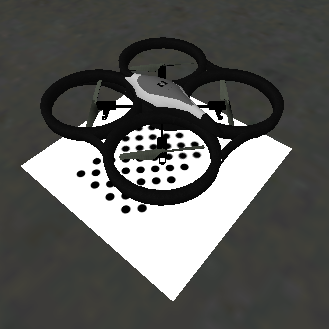
\includegraphics[width=6cm]{images/usarsim_camera_calibration.png}
\caption{Calibration of a virtual camera inside the USARSim simulator.} 
\label{fig:3Dmodel}
\end{figure}

USARSim supports dynamic lightning to produce realistic images and shadows.
However, the camera sensor lacks a noise model and doesn't emulate the effect of automatic white balancing that is performed in most cameras (including the AR.Drone's camera).
\cite{Visser2011imav} Briefly describes the influence of white balancing on image stitching and how to mimic the real images as close as possible.


		\subsection{Visual model}
In addition to the motion and sensor model, a visual model of the AR.Drone has been developed.
A highly detailed 3D model of the AR.Drone was provided by Parrot SA.
However, this model was unsuitable for simulation due to the computational complexity.
A simplified model (Figure~\ref{fig:3Dmodel}) was made using Blender\footnote{\url{http://www.blender.org/}}.
This model is optimized for simulation on consists of only 3142 vertices.
Both the simulated and real system have the same dimensions $(0.525,0.515,0.115)\small{m}$.
%The collision box (bounding box) was set

\begin{figure}[htb!]
\centering
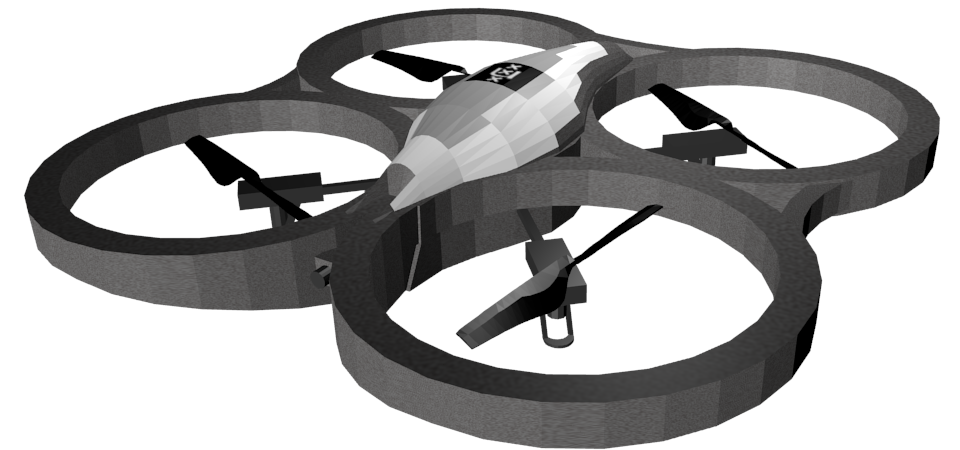
\includegraphics[width=6cm]{images/ardrone_blender_final.png}
\caption{3D model of the Parrot AR.Drone. This is a model optimized for simulation, based on the highly detailed model provided by Parrot SA.} 
\label{fig:3Dmodel}
\end{figure}


\section{Proposed framework}
\label{sec:proposed-framework}
The AR.Drone API (Section \ref{sec:API}) is the reference project for developing applications for the AR.Drone.
It provides basic functionality for communicating with the AR.Drone.
In order to perform advanced tasks (e.g., sensor data processing and automated drone control), a framework is proposed.
This framework includes an abstraction layer to abstract from the actual device.
Interfaces are used to connect the framework to an actual or virtual device.
Due to this abstraction, both the real and simulated AR.Drone can be used to validate the methods presented in the next chapter.

The main functionalities of the framework can be summarized as follows:
\begin{itemize}
\item Object-oriented programming: robots are represented with an object and are configured using parameters;
\item Abstraction from actual device: both the real and simulated AR.Drone can be connected to the framework;
\item Dataset recording and playback;
\item Queued sensor data and camera frame processing;
\item Keyboard controls;
\item Autonomous waypoint navigation;
\item Realtime 3D map visualization with freeflight
\end{itemize}

\begin{figure}[htb!]
\centering
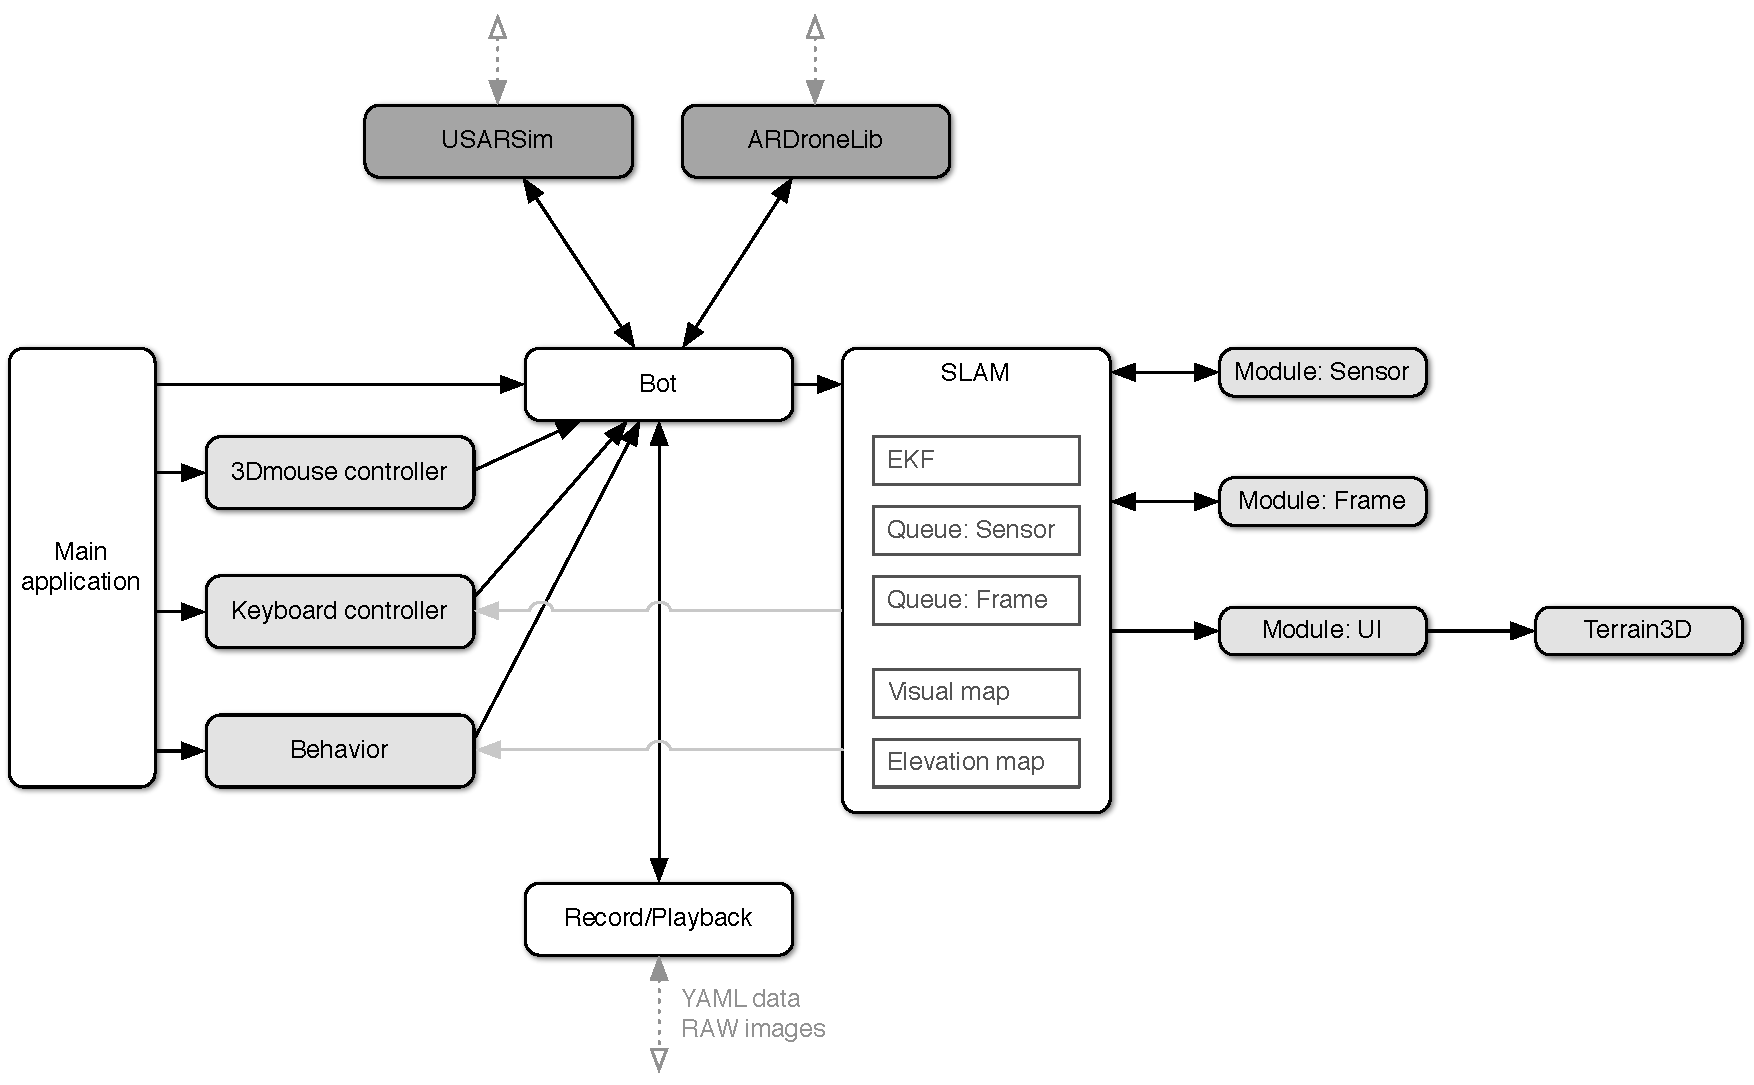
\includegraphics[width=\linewidth]{images/framework.pdf}
\caption{Schematic overview of the proposed framework. Each node respresents an object/datastructure. A light-gray node indicates the object is running in a dedicated thread. A dark-gray node indicates an interface to a device.} 
\label{fig:proposed_framework_schematic}
\end{figure}

A schematic overview of the framework is given in Figure \ref{fig:proposed_framework_schematic}.
The heart of the framework is the bot object, which respresents a robot.
Multiple robots can be instantiated simultaneous (e.g., a real and simulated AR.Drone).
The framework is limited to a single real AR.Drone's due to the lack of multirobot support in the ARDroneLib.
A robot is controlled by calling member functions of the corresponding bot instance.
Currently, three control methods are implemented: a \textit{keyboard controller}, a \textit{3D Mouse controller} and a \textit{behavior controller}.
Both the \textit{keyboard controller} and \textit{3D Mouse controller} can be used to manually fly the AR.Drone and manipulate the behavior of the SLAM system.
The \textit{behavior controller} is used to autonously fly the AR.Drone. 
It provides waypoint navigation to autonomously navigate the AR.Drone along a predefined route in world coordinates.
Feedback from the SLAM system (e.g., robot's estimated state) is used by the behavior controller to select the appropriate commands for the robot.

In addition to the controllers, a record and playback functionality is present.
Playback of a dataset is a valuable asset for testing.
All control commands sent to the drone and data received from the drone (i.e., navdata and camera frames) can be recorded to a dataset.
The data is stored in YAML\footnote{\url{http://en.wikipedia.org/wiki/YAML}} format.
When playing back a dataset, the data is pushed to the bot object in a way similar to regular data.
A timer is used to push the data at the appropriate timestamps, mimicing the original data as closely as possible.

An abstraction layer is used to abstract a bot from the actual device.
This enables to control both a real and simulated AR.Drone in the same manner.
\textit{Interfaces} are used to map a bot object to a (simulated) device.
When a bot object is instantiated, an interface has to be selected.
This can be either a real AR.Drone (using the ARDroneLib), simulated AR.Drone (USARSim) or use no interface for dataset playback (i.e., there is no communication with a robot).
The interface is responsible for transforming data received in device-specific format to a generic datastructure used by the framework.
Also, the control commands that are sent to the robot are transformed from generic format to device-specific format.

The data received from a robot (i.e., navdata and camera frames) is pushed to the SLAM object, which implements a SLAM system.
Navdata is added to the Sensor Queue, camera frames are added to the Frame Queue.
If the Frame Queue is not empty when a new frame is received (i.e., another frame is being processed), the frame is dropped by default.
The advantages of a queue are twofold: it allows data buffering and passing data to another thread to prevent blocking.
The latter is very important for a SLAM system, since blocking causes wasted data or delayed data.
The SLAM object has three modules: Sensor, Frame and UI.
Each module runs in a separate thread to prevent blocking and allow simultaneous data processing.
Both the Sensor and Frame module are able to update the EKF independently.

The \textbf{Sensor module} processes navdata (e.g., altitude and velocity estimates) from the AR.Drone at $200 \small{Hz}$.
When a navdata package is received, the EKF predicts a new state from the previous estimate (Section \ref{sec:background-solution-techniques}).
Each navdata package is processed before it can be used to update the estimated state of the AR.Drone.
This processing task includes the transformation of measurements to the global reference frame and the detection of obstacles.
The processed navdata is used to generate a measurement for the EKF.
Elements of the measurement matrix that cannot be (reliably) extracted from the processed navdata, are extraced from the prediced state and added to the measurement matrix with a higher covariance (uncertainty).
Finally, the measurement is used to update the state of the EKF.

The \textbf{Frame module} processes camera frames.
When a camera frame is received, the EKF predicts a new state from the previous estimate (Section \ref{sec:background-solution-techniques}).
Each camera frame is processed to extract information that is used to update the estimated state of the AR.Drone.
Processing includes Visual Odometry (Section \ref{sec:visual-slam-visual-odemetry}), updating the map (Section \ref{sec:mapping}) and recovering the global position of the AR.Drone by matching the frame against the map (Section \ref{sec:localization}).
The extracted information (i.e., velocities or global position) is used to generate a measurement for the EKF.
Elements of the measurement matrix that are be extracted from the camera frames (e.g., altitude), are extraced from the prediced state and added to the measurement matrix with a higher covariance (uncertainty).
Finally, the measurement is used to update the state of the EKF.

Processing a single frame may take up to $200 \small{ms}$ and causes a delay between input and updating the state.
This introduces a synchronization issue between state updates: when a update from the Frame module is applied, the estimated state is already updated by the Sensor module with more recent information that originates from the navdata.
This issue is solved by pausing the Sensor module (processing) while processing a frame.
After the state update by the Frame module is applied, the Sensor module is resumed and the queued navdata information is processed.

The \textbf{UI module} is responsible for visualizing the map.
It initializes a Terrain3D object and pushes local map updates to it.
The Terrain3D object renders the map (Figure \ref{fig:terrain3d_map}).
It allows 3D rendering of a textured elevation map.
Both the visual map and elevation map are integrated to a single map.
The code is based on the work by Chad Vernon \footnote{\url{http://www.chadvernon.com/blog/resources/directx9/moving-around-a-3d-world}} and uses DirectX 9 for rendering.
The estimated position of the AR.Drone is visualized with a red arrow.
\begin{figure}[htb!]
\centering
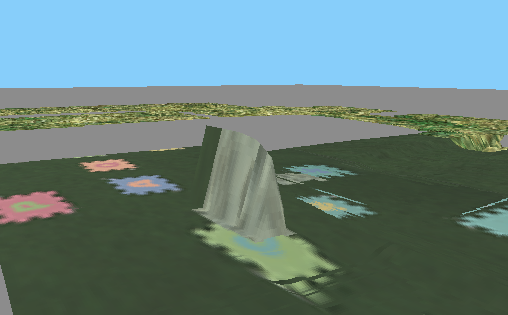
\includegraphics[width=6cm]{images/3dterrain_map.png}
\caption{Textured elevation map rendered by the Terrain3D object.} 
\label{fig:terrain3d_map}
\end{figure}



\chapter{Visual SLAM with the AR.Drone}
\label{chapter:visual-slam}
This chapter presents methods to build a visual map and how to use this map to make the AR.Drone localize itself.
In order to initialize a visual localization and mapping algorithm, a good estimate of the position based on the internal sensors of the AR.Drone is essential.
Section \ref{sec:pose_estimation} describes multiple methods to estimate the pose.
When an estimate of the pose is available, a map can be constructed using the method described in Section \ref{sec:mapping}.
Section \ref{sec:localization} described how this map is used by the AR.Drone to localize itself and reduce the errors pose estimates.
Finally, Section \ref{sec:elevation_map} describes an experimental method to build an elevation map using a single ultrasound sensor.

	\section{Pose estimation}
	\label{sec:pose_estimation}
%In order to initialize a visual localization and mapping algorithm, a good estimate of the position based on the internal sensors of the AR.Drone is essential.
The AR.Drone has several sources of information available about its movements and the majority of its computing power is dedicated to combine these sources into combined estimates. Here this information is combined into a state vector, with all information needed to initialize visual localization and mapping.

The AR.Drone is equipped with a number of sensors, which give frequent updates about the motion. 
The inertial sensor measures the body accelerations and angular velocities.
A proprietary filter on board of the AR.Drone converts the angular velocities to an estimated attitude (orientation).
A sonar sensor is used to measure the altitude of the vehicle.
In addition to the body accelerations, the AR.Drone sends an estimate of its estimated body velocity.
This estimate is based on the inertia measurements and optical flow obtained from the relative motion between camera frames.
%Unfortunately, the details of this velocity estimation are
%currently
%not documented by the manufacturer.
The details of this algorithm are proprietary information of the manufacturer. 

The information from the sensors are used in an Extended Kalman Filter (EKF) to estimate the current position.
The EKF has been considered~\cite{julier2004unscented} the facto standard in the theory of nonlinear state estimation.
Our EKF state vector comprises a position vector $p^{W}$, velocity vector $v^{W}$, acceleration vector $a^{W}$ and attitude (orientation) vector $q^{W}$.
All vectors are 3-dimensional Cartesian coordinates.

\begin{equation}
x = [ p^{W}  v^{W}  a^{W}  q^{W} ]
\label{eq:EKF_state_vecor}
\end{equation}

The filtered attitude (orientation) from the proprietary onboard filter is written directly to the attitude vector $q^{W}$ of the state.
%This is possible because 
Steder et al. \cite{steder2008visual} found that roll and pitch measurements are accurate, even for low-cost sensors and can be directly integrated into the state.
The body accelerations can be used to estimate the current velocity of the vehicle.
%However, from experiments \ref{Section sec:exp_accel} we found that the low-cost acceleration sensor from the AR.Drone provides unreliable data.
However, we found that the low-cost acceleration sensor from the AR.Drone provides unreliable data.
This is modeled by a large uncertainty in the covariance matrix $Q$ of the EKF.

Unlike the acceleration data, the velocity estimate sent by the AR.Drone is accurate enough for integration into the state.
Based on the previous position $p_{t-1}$, the state's velocity $v_{t}$ and time between measurements, the new position $p_{t}$ can be calculated as follows:

\begin{equation}
p_{t} = p_{t-1} + v_{t} \times \Delta t + a_{t} \times 0.5 \Delta t^2
\end{equation}
where $\Delta t$ is the variable time (seconds) between the last two measurements.
The body accelerations or velocity is sufficient to estimate the vehicle's altitude.
However, the sonar's altitude measurement can be integrated into the EKF to improve the altitude estimate.
The sonar sensor is not sensitive to drift because it provides an absolute altitude measurement.
Relying only on the sonar sensor is not optimal since the measurements depend heavily on material and structure of the floor.


		\subsection{Inertia measurements}
		\subsection{Onboard filtered measurements}
		\subsection{Vision-based velocity}

	\section{Mapping}
	\label{sec:mapping}
This visual map consists of a texture map and a feature map. The texture map is used for human navigation and the feature map is used by the AR.Drone to localize itself.

	\subsection{Visual map}
Now that we have an estimate of the AR.Drone's position and attitude in the world, we can use this information to build a visual map of the environment.
The AR.Drone is equipped with a down-looking camera that has a resolution of $176 \times 144$ pixels.
The frames captured by this camera can be warped on a flat canvas to create a visual map.
Directly merging the frames on the canvas is not possible, because individual frames can be taken from a broad range of angles and altitudes.
Instead, perspective correction is applied and all frames are normalized in size and orientation.

Before describing how a frame is warped, some basics about image formation are explained. %the camera matrix are explained.
The AR.Drone's camera is modeled using a pinhole camera model (Figure \ref{fig:mapping1}).
In this model, a scene view is formed by projecting 3D points into the image plane using a perspective transformation.
3D camera coordinates are typically described with homogeneous coordinates.

\begin{figure}[htb]
\centering
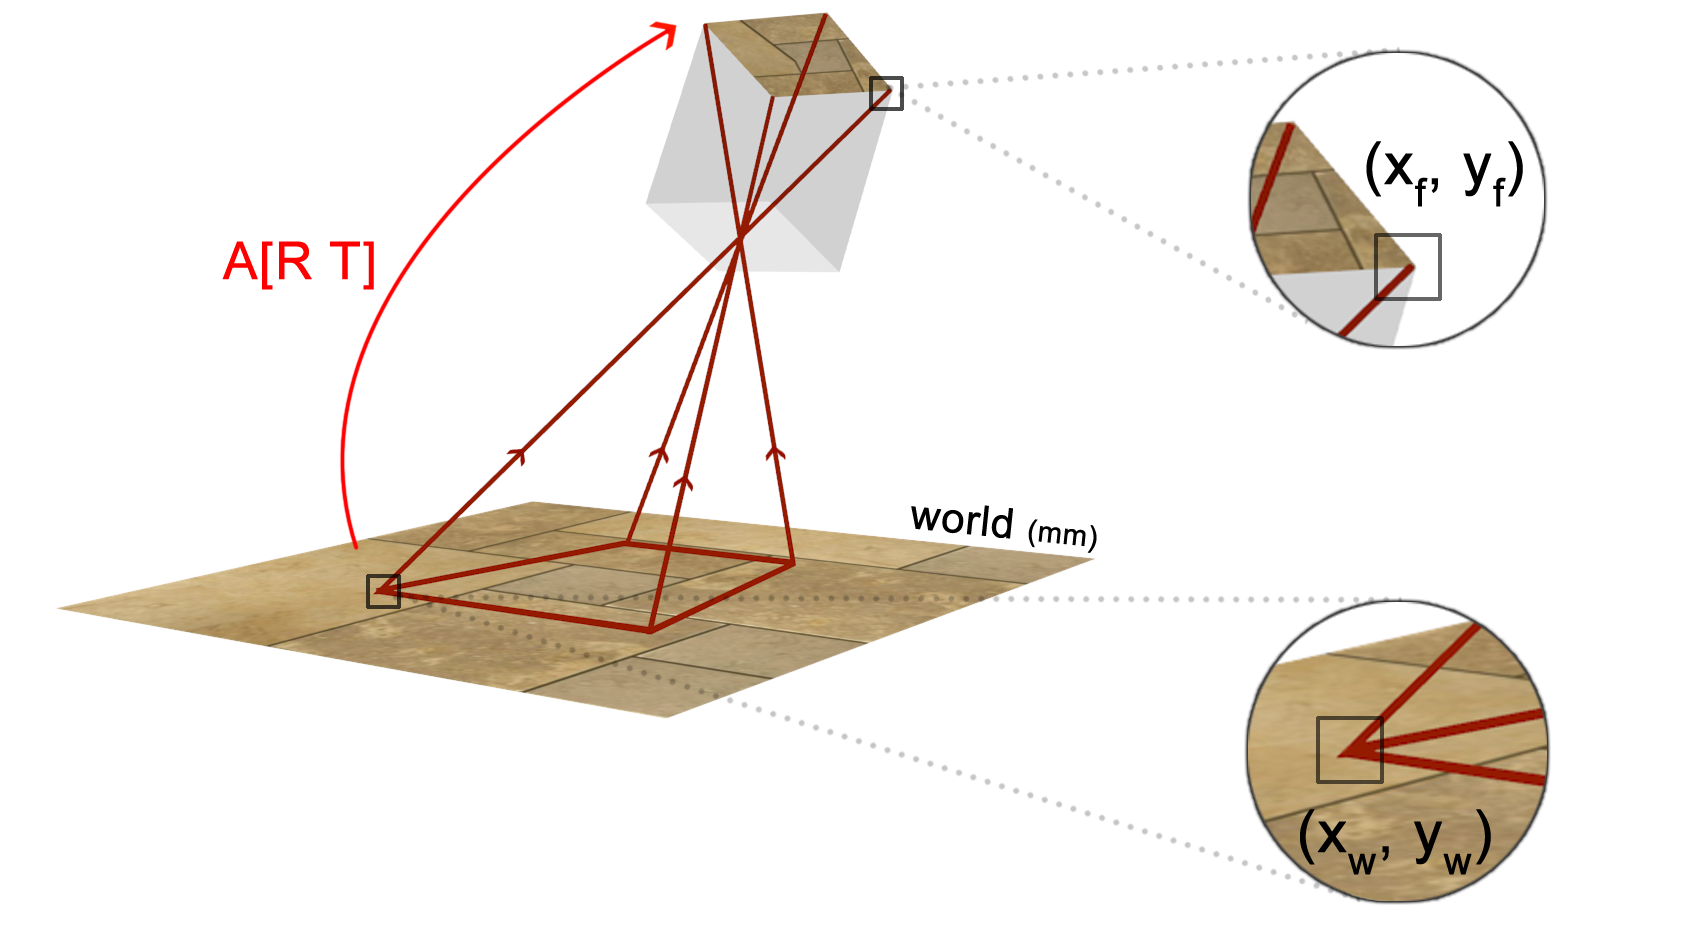
\includegraphics[width=10cm]{images/mapping0.png}
\caption{In the pinhole camera model, a scene view is formed by projecting 3D points into the image plane using a perspective transformation.}
\label{fig:mapping1}
\end{figure}

\begin{equation}
\left[ {
\begin{array}{c} x_f \\ y_f \\ 1 \end{array}
} \right]
= A[R|t]
\left[ {
\begin{array}{c} x_w \\ y_w \\ z_w \\ 1 \end{array}
} \right]
\end{equation}
where $x_f$ and $y_f$ represent a 2D point in pixel coordinates and $x_w$, $y_w$ and $z_w$ represent a 3D point in world coordinates.
The $3 \times 3$ \textit{camera intrinsic} matrix $A$ includes the camera's focal length and principal point.
The $3 \times 4$ joint rotation-translation matrix $[R|t]$ includes the \textit{camera extrinsic} parameters, which denote the coordinate system transformations from 3D world coordinates to 3D camera coordinates. Equivalently, the extrinsic parameters define the position of the camera center and the camera's heading (attitude) in world coordinates.

\begin{figure}[htb]
\centering
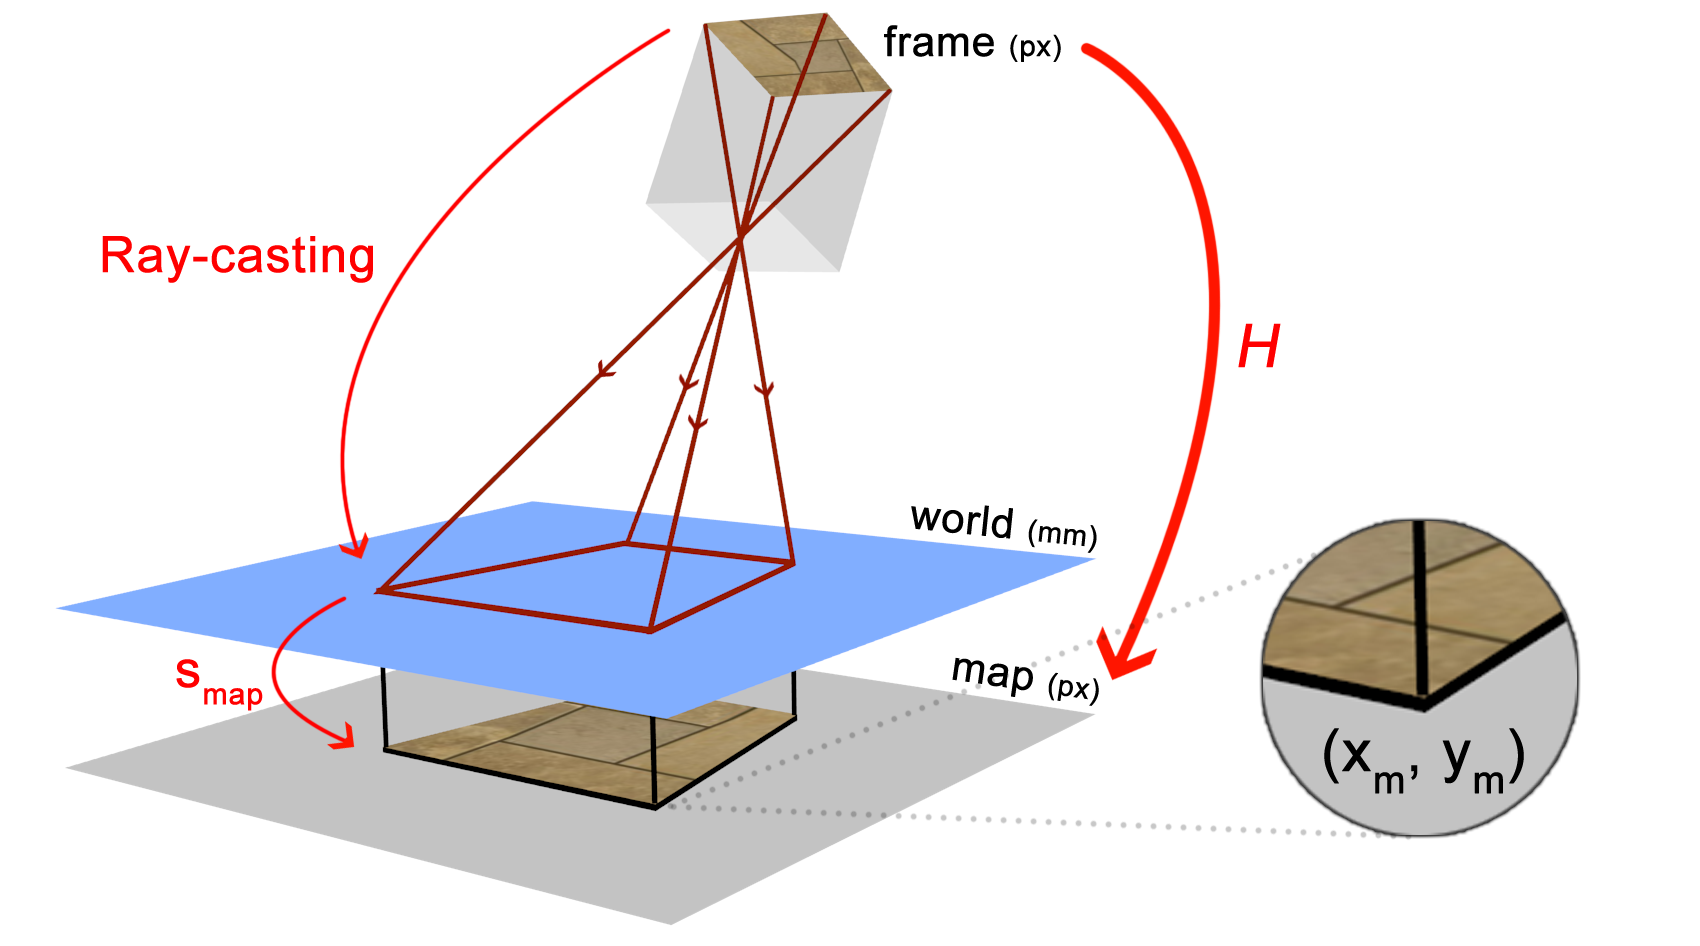
\includegraphics[width=10cm]{images/mapping1.png}
\caption{Visual map: warping a camera frame on the map's canvas. The frame's corners ($\small{px}$) are mapped to 2D world coordinates that lie on the world's plane. The 2D world coordinates of the frame are mapped to the map's canvas coordinates ($\small{px}$).}
\label{fig:mapping2}
\end{figure}

In order to warp a camera frame on the correct position of the canvas, we need to know which area of the world (floor) is captured by the camera.
This is the inverse operation of the image formation described above.
Instead of mapping 3D world coordinates to 2D pixel coordinates, 2D pixel coordinates are mapped to 3D world coordinates ($\small{mm}$).
It is impossible to recover the exact 3D world coordinates, because a pixel coordinate maps to a line instead of a point (i.e., multiple points in 3D world coordinates map to the same 2D pixel coordinate).
\begin{comment}
This is represented in the scaling factor $s$ in the next equation:

\begin{equation}
s \cdot \left[ {
\begin{array}{c} x_w \\ y_w \\ z_w \\ 1 \end{array}
} \right]
= A^{-1}[R|t]
\left[ {
\begin{array}{c} x_f \\ y_f \\ 1 \end{array}
} \right]
\end{equation}
\end{comment}
This ambiguity can be resolved by assuming that all 3D world points lie on a plane ($z_w = 0$), which makes it possible to recover $x_w$ and $y_w$.
The 2D world coordinates of the frame's corners are obtained by casting rays from the four frame's corners (top of Figure \ref{fig:mapping2}).
The 2D world coordinate that corresponds to a frame corner is defined as the point $(x_w,  y_w , 0)$ where the ray intersects the world plane ($z_w = 0$).

\begin{equation}
\left[ {
\begin{array}{c} x_w \\ y_w \\ 0 \end{array}
} \right]
 = \frac{(p_0 - l_0) \cdot n}{l \cdot n}
\end{equation}
where $n = \left[ {  \begin{array}{l l l} 0 & 0 & -1 \end{array}  } \right]^T$ is a normal vector to the world plane and $p_0 = \left[ {  \begin{array}{l l l} 0 & 0 & 0 \end{array}  } \right]^T$ is a point on the world plane.
$l$ is a vector in the direction of the ray and $l_0 = p^W$ is a point where the ray intersects the camera plane.
$l$ is computed as follows:

\begin{equation}
l = 
\left|
R
A^{-1}
\left[ {
\begin{array}{c} x_f \\ y_f \\ 1 \end{array}
} \right]
\right|
\end{equation}

Both the camera's extrinsic and intrinsic parameters are required for this operation.
The extrinsic parameters (position and attitude of the camera) are provided by the EKF state vector.
The camera intrinsic parameters are estimated using OpenCV's camera calibration tool\footnote{\url{http://opencv.itseez.com/modules/calib3d/doc/camera_calibration_and_3d_reconstruction.html}}. The implementation is based on the work from \cite{Zhang2000, Bouguet1999}.

%\footnotetext[3]{\url{http://opencv.itseez.com/modules/calib3d/doc/camera_calibration_and_3d_reconstruction.html}}

Now, a relation between the pixel coordinates and world coordinates is known.
However, the 2D world coordinates ($\small{mm}$) need to be mapped to the corresponding 2D pixel coordinates $(x_m, y_m)$ of the map's canvas.
%In the next phase, each frame corner in 2D world coordinates is mapped to the corresponding 2D position on the map's canvas.
A canvas with a fixed resolution of $4.883\small{mm/px}$ is used.
%This means that 1 pixel on the map's canvas corresponds to $4.883\small{mm}$ in world coordinates.

\begin{equation}
\left[ {
\begin{array}{c} x_{m} \\ y_{m} \end{array}
} \right]
= s_{map} \cdot
\left[ {
\begin{array}{c} x_{w} \\ y_{w} \end{array}
} \right]
\end{equation}
where $s_{map} = 1 / 4.884$.

Now, the map's pixel coordinates of the frame corners are known (bottom of Figure \ref{fig:mapping2}).
In order to transform a frame to the map's canvas, a relation between the frame's pixels and map's pixels is required.
A transformation from the frame's corner pixel coordinates and the corresponding pixel coordinates of the map's canvas can be computed.

\begin{equation}
\left[ {
\begin{array}{c} x_{m,i} \\ y_{m,i} \\ 1 \end{array}
} \right]
\sim
H
\left[ {
\begin{array}{c} x_{f,i} \\ y_{f,i} \\ 1 \end{array}
} \right]
\end{equation}

The local perspective transformation $H$ is calculated by minimizing the back-projection using a least-squares algorithm.
We used OpenCV's \textit{findHomography}\footnotemark[3] to find the perspective transformation.
This transformation describes how each frame's pixel needs to be transformed in order to map to the corresponding (sub) pixel of the map's canvas.
The transformation is used to warp the frame on the map's canvas.
By warping the frame on a flat canvas, implicit perspective correction is applied to the frames.
We used OpenCV's \textit{warpPerspective}\footnote{\url{http://opencv.itseez.com/modules/imgproc/doc/geometric_transformations.html}} to warp the frame on the map's canvas.

In this way a texture map can be built. This map consists of a set overlapping textures. The placement and discontinuities of the overlapping textures could be further optimized by map stitching, as described in \cite{Visser2011imav}. Here the texture map is used for human navigation. For automatic navigation a feature map is used, as described in the next section.

[REFER TO PAPER - map stitching]

			%\subsubsection{Map stitching}
			\subsubsection{Pose-based mapping}
			\subsubsection{Optimizing the map}


		\subsection{Feature map}
\label{sec:feature_map}
In addition to the visual map described above, a grid of image features (feature map) is created using a method we have developed.
This feature map will be used for localization purposes, as described in Section~\ref{sec:localization}.
The inertia measurements provide frequent position estimates.
%However, drift will increase the inaccuracy over time.
%However, drift will decrease the accuracy over time.
If the AR.Drone is able to relate a video frame to a position inside the feature map, the vehicle is able to correct this drift long enough to build a map 
as large as the indoor arena of the IMAV competition (as described in Section~\ref{sec:results}).

\begin{figure}[htb]
\centering
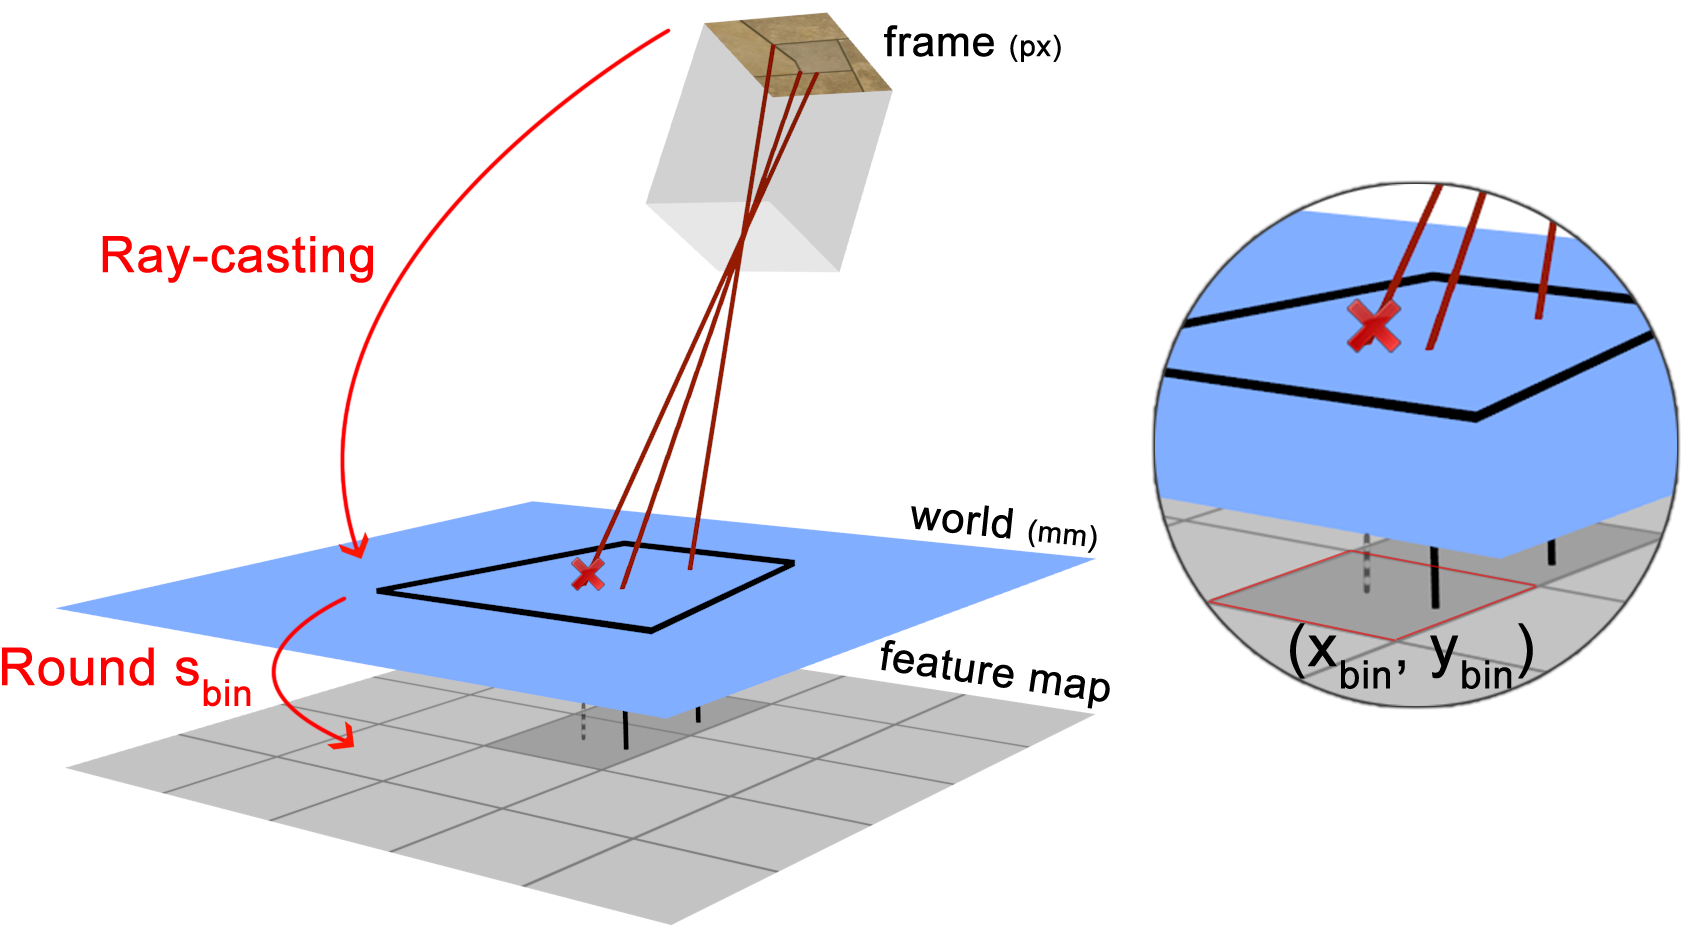
\includegraphics[width=10cm]{images/mapping3.png}
\caption{Feature map: adding visual features to a feature grid. Each feature found in the camera frame is mapped to the corresponding 2D world coordinates. The 2D world coordinates are mapped to the grid cell the feature belongs to. For each cell, only the best feature is stored.}
\label{fig:mapping3}
\end{figure}

A 2D grid with a fixed resolution of $100 \times 100mm$ per cell is used.
%which is nearly equivalent with $20 \times 20\small{px}$.
%Each grid cell corresponds to an area of $100 \times 100\small{mm}$ of the world.
From each camera frame we extract Speeded-Up Robust Features (SURF) \cite{Bay2008cviu} that are invariant with respect to rotation and scale.
% SURF features are scale- and rotation-invariant. See Bay2008cviu
Each feature is an abstract description of an "interesting" part of an image (e.g., corners).
A feature is described by a center point in image sub-pixel coordinates and a descriptor vector that consists of 64 floats.

Each feature that is detected in a camera frame is mapped to the corresponding cell of the feature map.
A feature's center point ($x_f, y_f$) is transformed to its corresponding position in 2D world coordinates ($x_w, y_w$), visible in the top of Figure \ref{fig:mapping3}.
This is done by casting a ray from the features pixel coordinates in the frame.
The method is similar to the method used for casting ray's from the frame's corners (Section \ref{sec:texture_map}).
Finally, the 2D world position ($x_w, y_w$) of each feature is transformed to the corresponding cell indices ($x_{bin}, y_{bin}$), visible in the bottom of Figure \ref{fig:mapping3}.

\begin{equation}
\left[ {
\begin{array}{c} x_{bin} \\ y_{bin} \end{array}
} \right]
=
Round(
s_{bin}
\cdot
\left[ {
\begin{array}{c} x_{w} \\ y_{w} \end{array}
} \right]
)
\end{equation}
where $s_{bin} = 0.01$.

For each cell, only the best feature (e.g. with the highest response) is kept and the other features are dropped.
%If a cell is already connected to a feature descriptor ($grid_{x,y} \neq \emptyset$), the cell is ignored.
If a cell already contains a feature descriptor ($grid_{x,y} \neq \emptyset$), the cell is ignored.

\begin{equation}
grid_{x,y} = 
\begin{cases}
\arg\max_{d \in D_{x,y}} response(d) & \mbox{if }  grid_{x,y} = \emptyset \\
grid_{x,y}   &   \mbox{else}
\end{cases} 
\end{equation}
where $D_{x,y}$ is the set of features that is mapped to cell $x_{bin} ,y_{bin}$.

%The remaining feature descriptors, including the corresponding world coordinates $x_w, y_w$, are added at the end of a descriptor matrix.
%The indices of these descriptors are written to the corresponding cell of the grid.
%This way, each cell of the grid is connected to a descriptor from the descriptors matrix.
The remaining (best) feature descriptors, including the corresponding world coordinates ($x_w, y_w$), are added to the corresponding grid cells.


\begin{comment}
\subsubsection{Processing time}

Processing a single frame and adding it to the map requires approximately $130\small{ms}$ (visual mapping: $20\small{ms}$, feature mapping: $110\small{ms}$).
The AR.Drone's framerate is fixed at 15fps, which is too high to process each single frame in realtime.
In order to achieve realtime mapping, frames that are receiving while another frame is still being process, are dropped.
However, the processing is sufficiently fast to enable seamlessly mapping.
For example, when flying at $1\small{m}$ altitude, the camera (64 degree FOV) perceives $1.24\small{m}$ floor.
The maximum horizontal speed to achieve seamlessly mapping at 15fps is 
% $(1.24 * 15 = 
$18.75\small{m/s}$, which is nearly four times the default maximum speed of the AR.Drone ($5\small{m/s}$).
With reduced framerate (7.7fps instead of 15 fps), the maximum horizontal speed is 
% $1.24 * 7.7 = 
$9.55\small{m/s}$, which is significantly faster than the AR.Drone's default maximum speed.
\end{comment}


	\section{Localization}
\label{sec:localization}

The feature map created in the previous section can be used for absolute position estimates, at the moment of loop-closure (when the AR.Drone is above a location where it has been before).
This allows to correct the drift that originates from the internal sensors of the AR.Drone.
The inertia measurements provide frequent position estimates.
However, the estimated position will drift over time, because the errors of the inertia measurements being accumulated.
The feature map that is created can be exploited to reduce this drift, because localization against this map provides absolute positions of the vehicle.
These absolute positions are integrated into the EKF and improve the estimated position and reduce the covariance of the state.

When a camera frame is received, SURF features are extracted.
Each feature consists of a center position in pixel coordinates ($x_f, y_f$) and a feature descriptor.
A feature's center point ($x_f, y_f$) is transformed to its corresponding position in 2D world coordinates ($x_w, y_w$), visible in the top of Figure \ref{fig:mapping3}.
This is done by casting a ray from the features pixel coordinates in the frame.
The method is similar to the method used for casting ray's from the frame's corners (Section \ref{sec:texture_map}).

%The pixel coordinates of the features are transformed to 2D world coordinates.
%The method used is already described in Section X.

The next step is matching the feature descriptors from the camera frame against the feature descriptors from the feature map.
When the feature map is quite large, this process becomes slow.
However, the estimated position of the vehicle can be used to select a subset of the feature map.
This can be done by placing a window that is centered at the vehicle's estimated position.
The covariance of the estimated position can be used to determine the size of the window.
The set of frame descriptors (query descriptors $D_q$) is matched against the map descriptors (training descriptors $D_t$).
Matching is done using a brute force matcher that uses the $L^2$ norm as similarity measure.
For each query descriptor $d_q$ from the frame, function $C(d_q)$ selects the training descriptor $d_t$ from the map that minimizes the $L^2$ norm:


\begin{equation}
C(d_q) = \arg\min_{d_t \in D_T} L2(d_q, d_t)
\end{equation}
where $D_T$ is the set of map descriptors within a window around the estimated position.
The $L2$ distance between two descriptors $a$ and $b$ is defined as:

\begin{equation}
L2(a,b) =\sqrt { \sum_{i=1}^{N} \left| a_i - b_i \right| ^2 }
\end{equation}
where $N = 64$ is the length of the SURF descriptor vector.

Each query descriptor (frame) is matched against the descriptor from the training descriptors (map) that is most similar.
Please note it is possible that multiple descriptors from the frame are matched against a single descriptor from the map.

For each match $C(d_q, d_t)$ the 2D world coordinates $(x_{w, d_q}, y_{w, d_q})$ and $(x_{w, d_t}, y_{w, d_t})$ of both descriptors are already computed.
These point pairs can be used to calculate a transformation between the query points (frame) and training (map) points.
This transformation describes the relation between the EKF estimated vehicle position (described in Section~\ref{sec:EKF}) and the position according to the feature map.

\begin{figure}[htb]
\centering
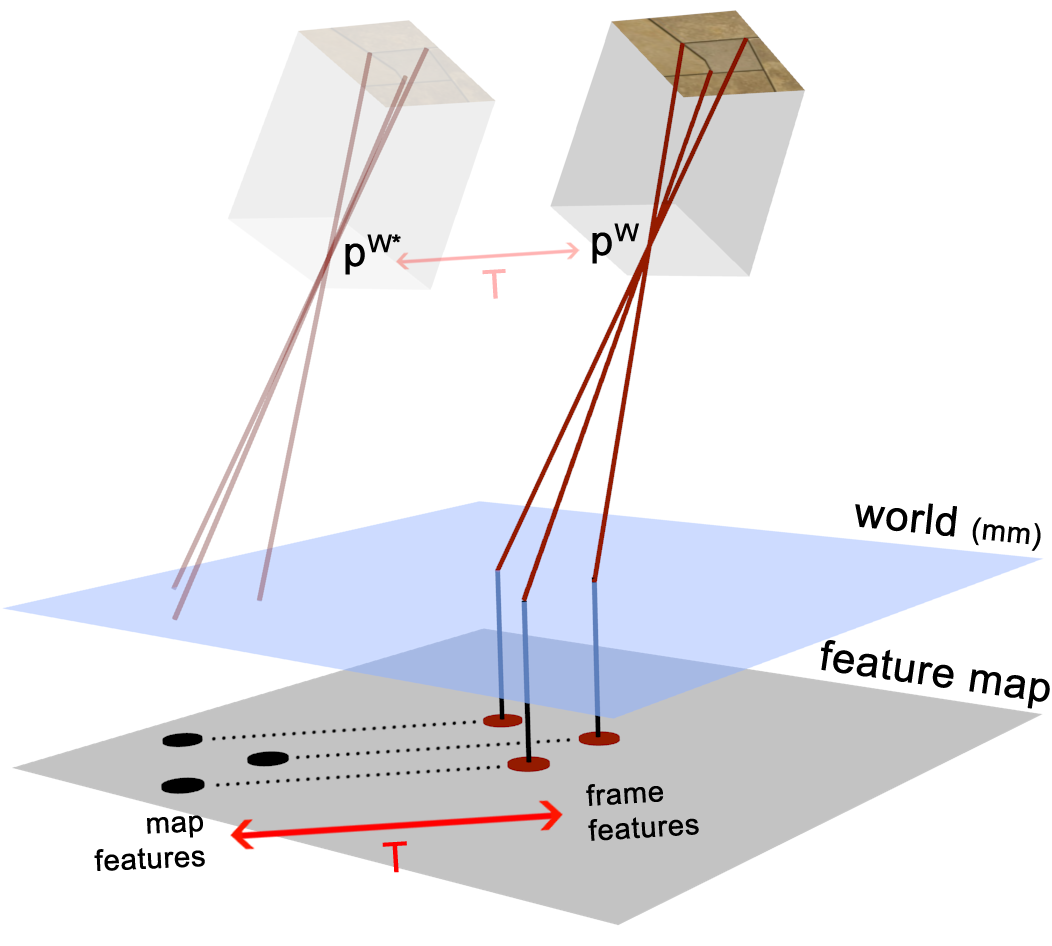
\includegraphics[width=9cm]{images/localization1.png}
\caption{Localization: features from the camera frame (red circles) are matched against the features from the feature map (black circles). All the feature points (pixels) are converted to 2D word coordinates. The translation $T$ between both feature sets is calculated and used to correct the estimated position of the AR.Drone.}
\label{fig:localization1}
\end{figure}

Different types of transformations can be used to describe the relation between the point pairs (e.g., perspective transformation or affine transformation).
However, if not all of the point pairs fit the transformation (due to outliers), the initial transformation estimate will be poor.
We use Random Sample Consensus (RANSAC) \cite{fischler1981random} to filter the set of matches in order to detect and eliminate erroneous matches (point pairs).
RANSAC tries different random subsets of corresponding point pairs.
It estimates the transformation using this subset and then computes the quality of the computed transformation by counting the number of inliers.

Since the point pairs are normalized,
%,(i.e., all pixel coordinates are transformed to 2D world coordinates),
the perspective deformation and scale differences between the point pairs (matches) are already removed.
The remaining degrees of freedom are the translation and rotation between the point pairs. 
Perspective transformation and affine transformation provide more degrees of freedom than required.
This is potentially dangerous, because an incorrect transformation may still results in a high percentage of inliers.
For example, this may happen when multiple query descriptors (frame) are matched against a single training descriptor (map).
In that case, a perspective or affine transformation is found that scales all points to a single position.
This transformation does not correspond with the actual translation and rotation, but is a valid transformation according to the RANSAC algorithm.

Instead of computing a full perspective, affine or Euclidean transformation, here only the translation in $x$ and $y$ direction is estimated. The rotation is estimated independently, as described at the end of this section.
The translation is estimated by taking a subset of 3 random point pairs.
The translation for those points is computed as follows:

\begin{comment}
$M_{train} = \begin{pmatrix}
x_{0,t,w} & y_{0,t,w}
\\
x_{1,t,w} & y_{1,t,w}
\\
x_{2,t,w} & y_{2,t,w}
\end{pmatrix}$

$M_{query} = \begin{pmatrix}
x_{0,q,w} & y_{0,q,w}
\\
x_{1,q,w} & y_{1,q,w}
\\
x_{2,q,w} & y_{2,q,w}
\end{pmatrix}$

\begin{equation}
T = (M_{train} - M_{query}) / N
\end{equation}


\begin{equation}
T =
\left[ {
\begin{array}{c}
 \frac{\sum_{i}^{N} (x_{t,w} - x_{q,w})}{N}
\\
 \frac{\sum_{i}^{N} (y_{t,w} - y_{q,w})}{N}
\end{array}
} \right]
\end{equation}


\end{comment}


\begin{equation}
T_x = \frac{\sum_{i}^{N} (x_{w, d_t, i} - x_{w, d_q, i})}{N}
\end{equation}
\begin{equation}
T_y = \frac{\sum_{i}^{N} (y_{w, d_t ,i} - y_{w, d_q, i})}{N}
\end{equation}
where $N = 3$ is the number of point pairs.

The standard deviation of translation  $T$ is defined as:

\begin{equation}
\sigma_x = \sqrt{  \sum_{i}^{N}   ((x_{w, d_t} - x_{w, d_q}) - T_x)^{2}   }
\end{equation}
\begin{equation}
\sigma_y = \sqrt{  \sum_{i}^{N}   ((y_{w, d_t} - y_{w, d_q}) - T_y)^{2}   }
\end{equation}

The confidence $c$ of translation $T$ is computed using the standard deviation:

\begin{equation}
c_{T} = 1 -   \sigma_x / \theta_{d} -  \sigma_y / \theta_{d}
\end{equation}
where $\theta_d$ = 200.

After RANSAC has performed all iterations, the translation with highest confidence $T_{best}$ is used as final translation.
A big advantage of this two degrees of freedom approach is that it is very efficient, allowing a great number of RANSAC iterations to find the optimal subset of point pairs.
If the confidence $c_{T}$ of the translation $T_{best}$ exceeds a threshold, the transformation $T$ is added to the estimated position $p^W$ to compute the corrected position $p^{W*}$. This corrected position is integrated in the EKF as measurement with low covariance.
Please note this method requires that the estimated yaw of the vehicle is close to the actual yaw.
A large difference between estimated and actual yaw results in low confidence $c_T$.
Localization on regular basis should sufficiently correct errors in the estimated yaw.

If the confidence is exceptionally high (i.e., good matches are found), the selected point pairs are used to determine the rotation between the estimated yaw and the real yaw of the vehicle. This rotation is used to correct the drift in yaw.
The rotation is computed using Kabsch algorithm \cite{Kabsch:a12999}.
This method computes the optimal rotation matrix that minimizes the RMSD (root mean squared deviation) between two paired sets of points.
Like the translation, the rotation is added to the estimated rotation to calculate the correct rotation. This rotation is directly written to the EKF state.

This localization method allows us to exploit the feature map created in Section~\ref{sec:feature_map} and get absolute position estimates which can be used to autonomously navigate the AR.Drone, as demonstrated in the next section.


		\subsection{Pose recovery approaches}
			\subsubsection{Correcting for translation}
			\subsubsection{Correcting for rotation}

	\section{Elevation mapping using an ultrasound sensor}
	\label{sec:elevation_map}
An elevation map can be used to improve navigation capabilities of both aerial and ground robots.
For example, ground robots can use elevation information to plan routes that avoid obstacles.
As stated in Section \ref{sec:related-research-elevation-mapping}, no publications were found that address the problem of elevation mapping using a single airborne ultrasound sensor.
%At first glance this seems unlikely, because a significant percentage of MAVs is equipped with an ultrasound sensor, commonly used for altitude stabilization.
%However, 
The fundamental limitations of an ultrasound sensor make it hard to build an elevation map.
Two issues are described below.

%\subsection{Fundamental issues}
The first issue is the unknow true altitude $z_{true}$ of the vehicle.
When a MAV is flying above a perfectly flat floor, the measured altitude $z_{sensor}$ is equal to the true altitude $z_{true}$.
However, when an obstacle comes in range of the ultrasound sensor, the measured distance $z_{sensor}$ decreases and is not equal to the true altitude $z_{true}$, meaning that $z_{true}$ cannot be derived from the ultrasound sensor directly.
When the true altitude is unknown, it is impossible to determine the floor's elevation from the distance measurements using the following equation:
\begin{equation}
elevation = z_{true} - z_{sensor}
\end{equation}
%When the MAV is flying above a flat floor without obstacles, the vehicle will remain at a fixed altitude $z$.
%However, when obstacles come in range of the ultrasound sensor, the measured distance $z_{sensor}$ decreases and the vehicle will increase its true %altitude $z_{true}$ by stabilizing the measured altitude $z_{sensor}$.
%Because $z_{sensor} \neq z_{true}$, the true altitude of the vehicle cannot be derived directly from the sensors.
%When the true altitude of the vehicle is unknown, it is hard to use distance measurements to determine the height of obstacles.

Another limitation of using an ultrasound sensor for elevation mapping is the resolution of the sensor.
As described in Section \ref{sec:ultrasound_altimeter}, an ultrasound sensor is unable to obtain precise directional information about objects.
Sound progragates in a cone-like manner.
Due to this property, the sensor acquires entire regions of constant depth instead of discrete depth points.
So, the ultrasound sensor can only tell there is an elevation at the measured distance somewhere within the measured cone.
This makes it hard to accurately determine the contours/borders of obstacles.

A third difficulty is related to the altitude stabilization of the AR.Drone (Section \ref{sec:platform-controls}).
The AR.Drone will change its absolute altitude when an altitude difference is detected.
This complicates the detection of elevations, since it cannot be assumed the absolute altitude will remain roughly the same when flying above an object.

The remaining part of this section describes a method to extract elevation information from an airborne ultrasound sensor.
The true altitude of the AR.Drone is modeled as the combination of the measured altitude $z_{sensor}$ and the elevation of the floor $\delta$ below the vehicle:
\begin{equation}
z_{true} = \delta + z_{sensor}
\end{equation}
where the elevation $\delta$ is unknown and needs to be recovered from the ultrasound measurements.
A key part of recovering $\delta$ is a finite-state machine that describes \textit{elevation events}.
A schematic overview of the finite-state machine is given in Figure \ref{fig:elevation_map_fsm}.
This finite-state machine has three different states: $\{ \text{NONE}, \text{UP}, \text{DOWN} \}$.
State NONE indicates no significant elevation changes are occuring, state UP indicates a significant increase of elevation is detected and state DOWN indicates a significant decrease of elevation is detected.

\begin{figure}[htb]
\centering
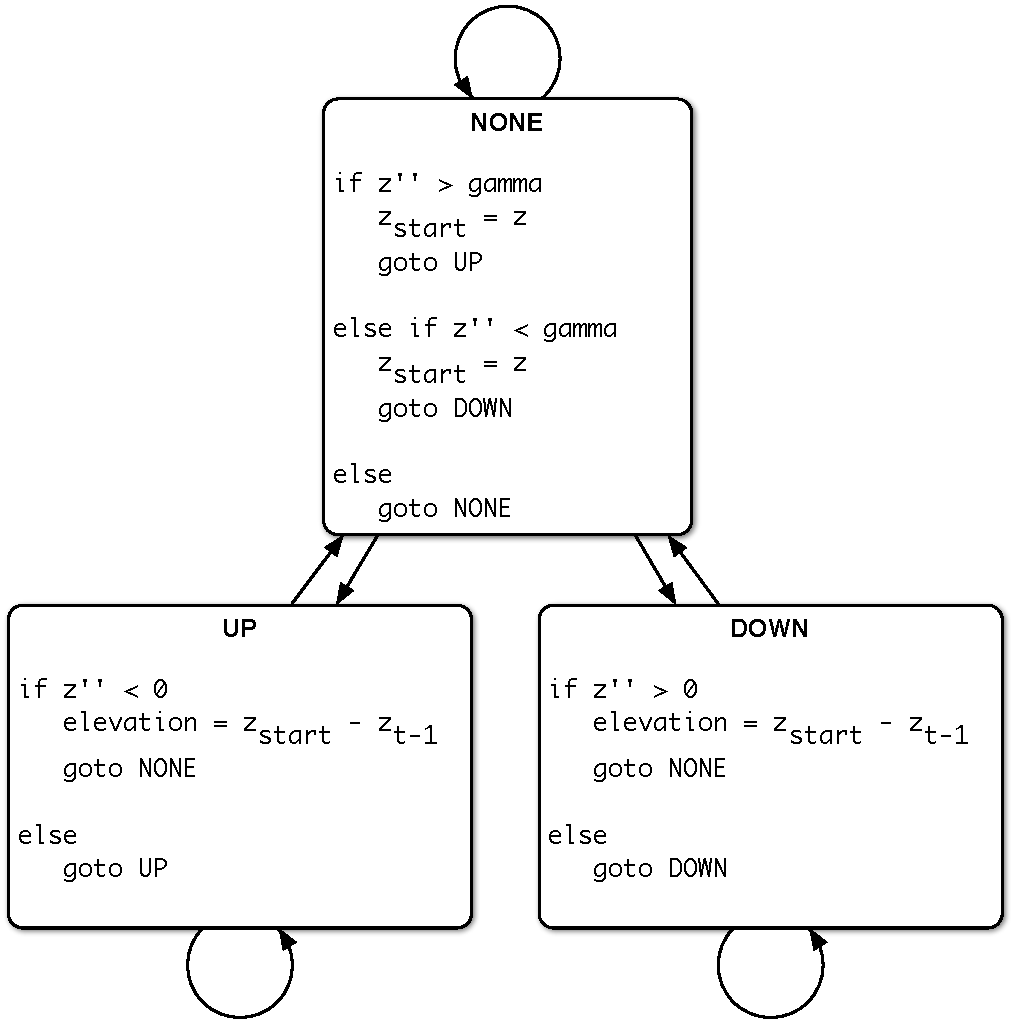
\includegraphics[width=10cm]{images/elevation_map_fsm.pdf}
\caption{Schematic overview of the finite-state machine used for elevation mapping. $z''$ is the second order derivative of the ultrasound distance measurement.}
\label{fig:elevation_map_fsm}
\end{figure}

Elevation changes are detected using a filtered second order derivative (acceleration) of the sonar measurement $z_{sensor}$.
Obstacles that enter or leave the range of the ultrasound sensor result in sudden changes in ultrasound distance measurements.
These changes are detected when the second order derivative exceeds a certain threshold $\gamma_{elevationEvent}$ and an elevation event is triggered.
The threshold $\gamma_{elevationEvent}$ was carefully chosen such that altitude corrections performed by the AR.Drone altitude stabilization are not detected as being elevation events.
In addition, the second order derivative is filtered by adding to the EKF state vector.
An elevation event ends when the sign of the second order derivative switches.
This happens when the AR.Drone altitude stabilization starts to change the absolute altitude to compensate for the change in measured altitude.
Now, the elevation change can be recovered by substracting the measured distance at the end of the elevation event from the measured distance before the elevation event was triggered:
\begin{equation}
\Delta\delta_{t} = z_{sensor, t-\Delta t-1} - z_{sensor, t-1}
\end{equation}
where $\Delta\delta_{t}$ is the elevation change during an elevation event, $\Delta t$ is the duration of an event, $z_{sensor, t-\Delta t-1}$ is the distance measurement before the event started and $z_{sensor, t-1}$ is the distance measurement when the event ended.
The total elevation is given by:
\begin{equation}
\delta_{t} = \delta_{t-1} + \Delta\delta_{t}
\end{equation}

\begin{figure}[htb!]
  \begin{center}
    \subfigure[Response]{\label{fig:elevation_method}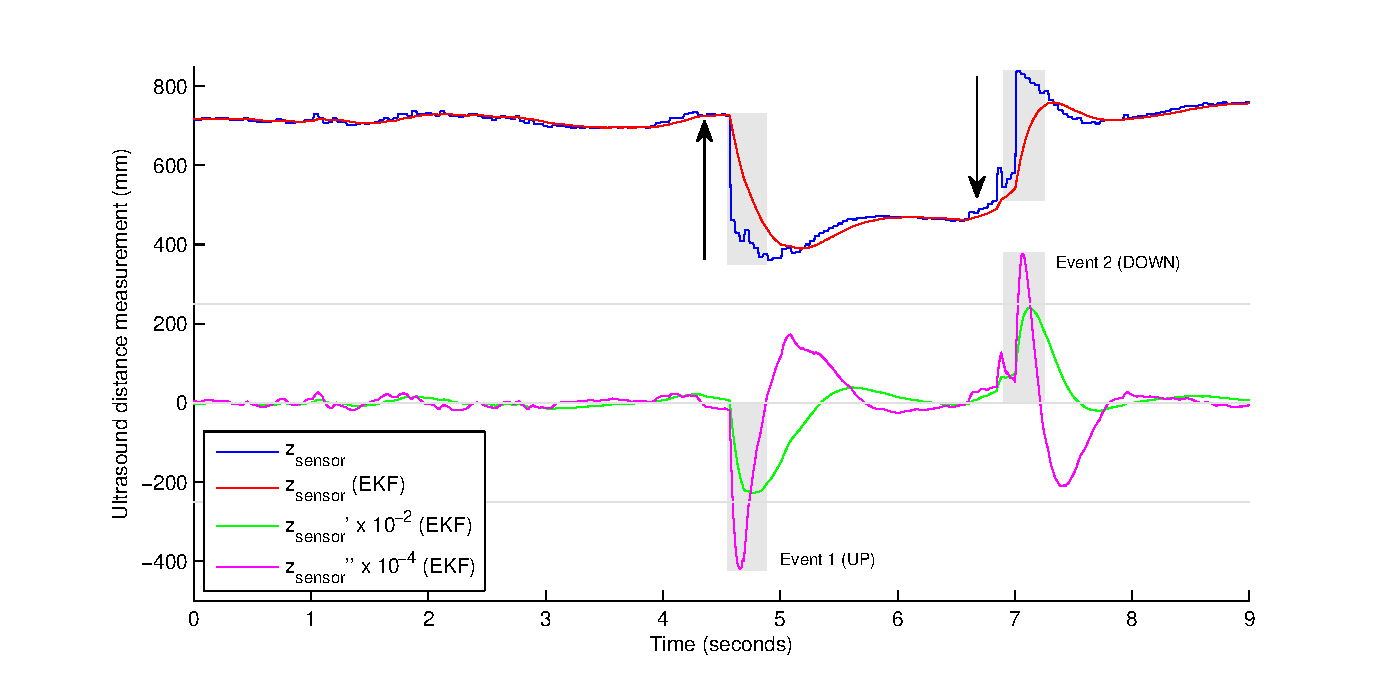
\includegraphics[width=\linewidth]{images/elevation_map.eps}}
    \subfigure[Corresponding elevation]{\label{fig:elevation_method_area}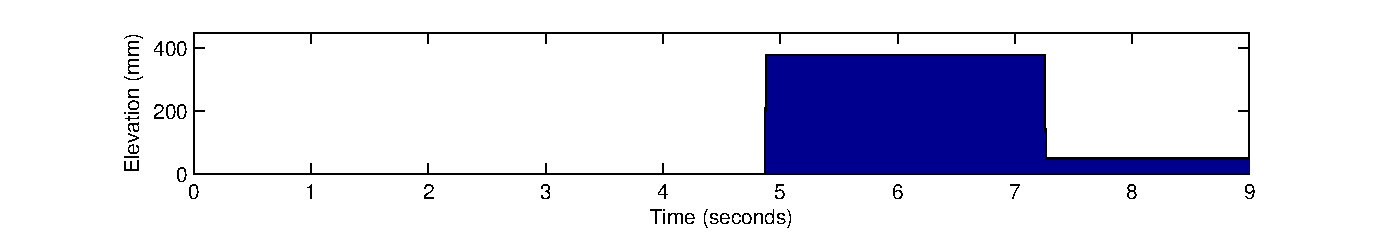
\includegraphics[width=\linewidth]{images/elevation_map_area.eps}}
 \end{center}
\caption{a) Response of the ultrasound sensor when flying over an object of approximately $(60,60,40)\small{mm}$. The lightgray lines indicate the threshold $\gamma_{elevationEvent}$ and null-line. When the second order derivative (magenta line) exceeds the threshold, an event is started (lightgrey rectangle). An event ends when the derivative swaps sign. Each arrow indicates the change in elevation caused by the event. The first event increases the elevation when entering an object and the second event decreases the elevation when leaving the object.
Between both events, the AR.Drone performs an altitude correction, as can be seen by the relatively slow increasement of distance. This increasement is not infomative about the elevation and is ingnored by the elevation mapping method.\\ b) Elevation $\delta$ below the AR.Drone over time. The elevation increases to approximately $40\small{cm}$ when flying above an obstacle. The elevation is decreased when the obstacle is out of the ultrasound sensor's range. There is a small error between both elevation events, resulting in a small false elevation ($\pm 50\small{mm}$) after the AR.Drone flew over the obstacle and is flying above the floor again.}
  \label{visual-slam-elevation-method}
\end{figure}

\begin{comment}
\begin{figure}[htb]
\centering
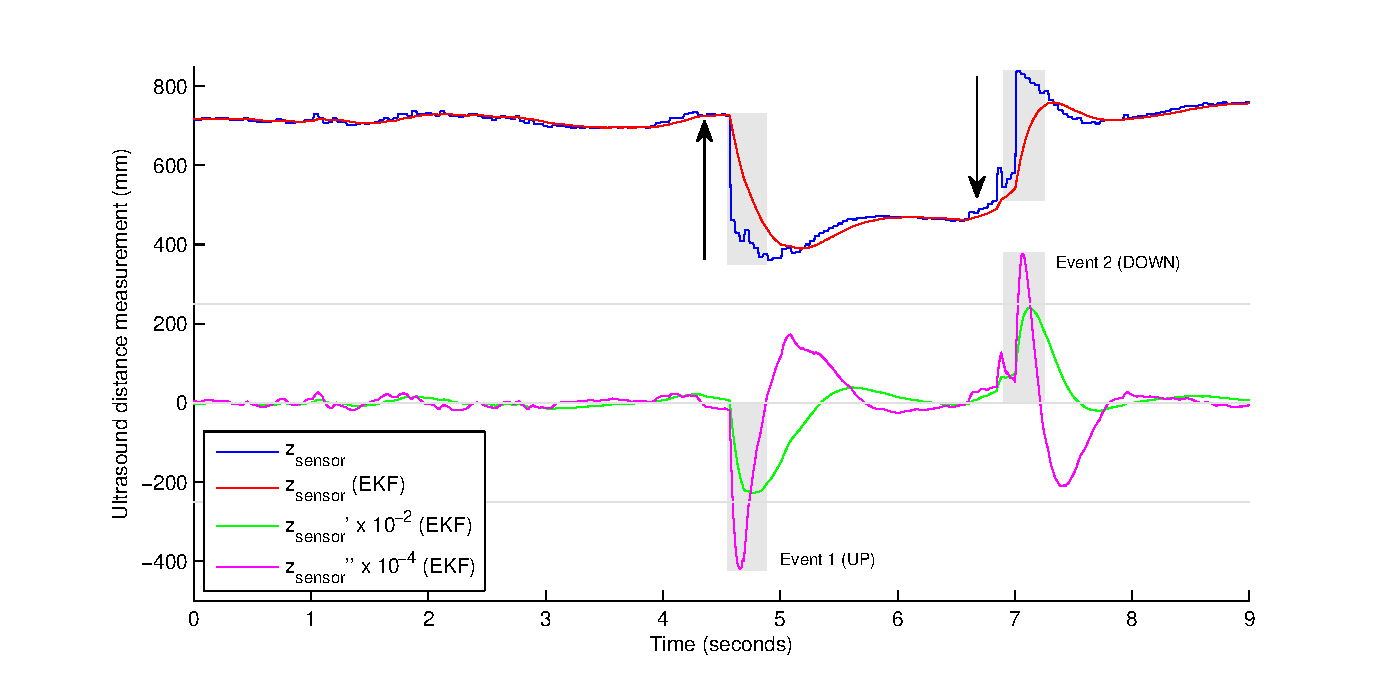
\includegraphics[width=\linewidth]{images/elevation_map.eps}
\caption{Response of the ultrasound sensor when flying over an object of approximately $(60,60,40)\small{mm}$. The lightgray lines indicate the threshold $\gamma_{elevationEvent}$ and null-line. When the second order derivative (magenta line) exceeds the threshold, an event is started (lightgrey rectangle). An event ends when the derivative swaps sign. Each arrow indicates the change in elevation caused by the event. The first event increases the elevation when entering an object and the second event decreases the elevation when leaving the object.
Between both events, the AR.Drone performs an altitude correction, as can be seen by the relatively slow increasement of distance. This increasement is not infomative about the elevation and is ingnored by the elevation mapping method.}
\label{fig:elevation_method}
\end{figure}
\begin{figure}[htb]
\centering
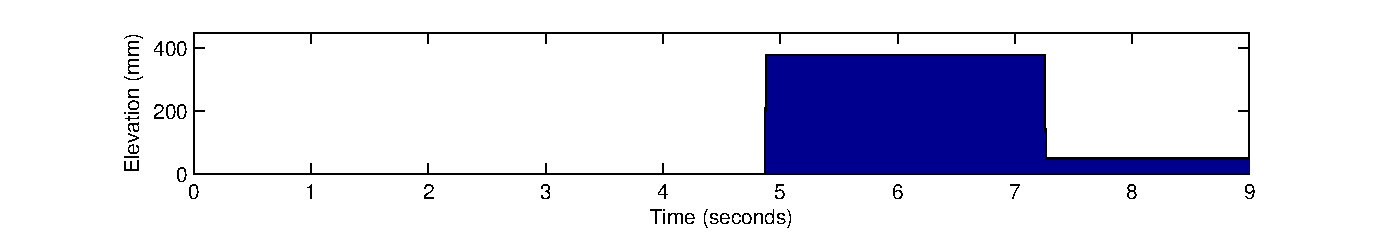
\includegraphics[width=\linewidth]{images/elevation_map_area.eps}
\caption{Elevation $\delta$ below the AR.Drone over time. The elevation increases to approximately $40\small{cm}$ when flying above an obstacle. The elevation is decreased when the obstacle is out of the ultrasound sensor's range. There is a small error between both elevation events, resulting in a small false elevation ($\pm 50\small{mm}$) after the AR.Drone flew over the obstacle and is flying above the floor again.}
\label{fig:elevation_method_area}
\end{figure}
\end{comment}

The elevation information is stored in a grid that is similar to the feature map described in Section \ref{sec:feature_map}.
For each ultrasound distance measurement, elevation $\delta_t$ is computed and stored in the grid cells that corresponds to the world coordinates where a line perpendicular to the AR.Drone body intersects the world plane.
These world coordinates are the position where the center of the ultrasound sensor's cone hits the floor.
Because the exact size of an object is unkown, the elevation is written to all grid cells within a radius $\gamma_{elevationRadius}$ around the intersection point.

This approach may lead to cases where the size of an obstacle is overestimated in the elevation map.
Therefore, an additional refinement step was added to the elevation mapping methods.
If no elevation is measured ($\delta_t \approx 0$), it can be assumed there is no obstacle inside the cone of the ultrasound sensor.
Using this assuption, all grid cells within the cone can resetted to zero elevation and locked to prevent future changes.
The radius of the cone is computed using the following equation:
\begin{equation}
r = tan (\alpha_{ultrasound} \times z_{sensor})
\end{equation}
where $r$ is the radius of a cone of height $z_{sensor}$ and $\alpha_{ultrasound}$ is the opening angle of the ultrasound sensor.

\begin{figure}[htb!]
  \begin{center}
	%\hspace*{-1.5cm}
\advance\leftskip-2.5cm\rightskip-2.5cm
    \subfigure[Blup]{\label{visual-slam-elevation-map1}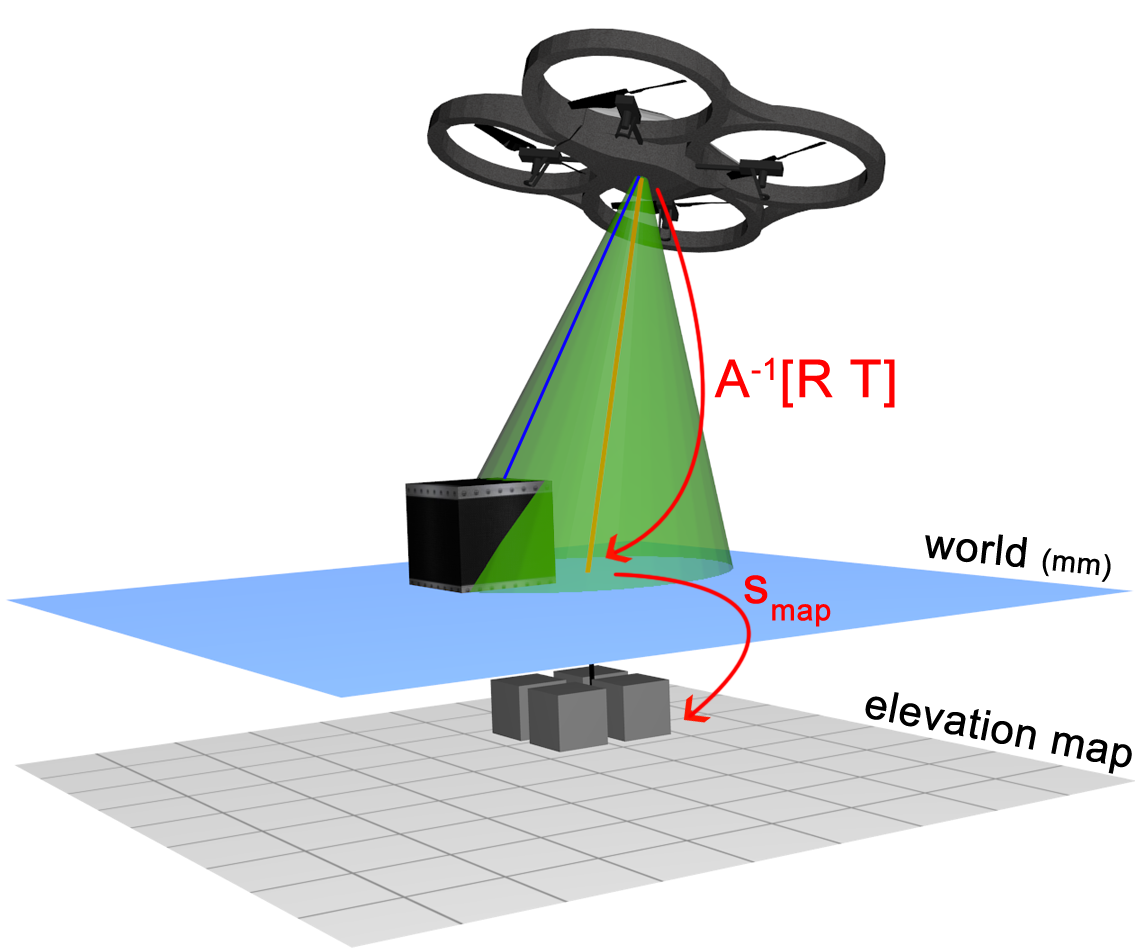
\includegraphics[width=0.4\linewidth]{images/elevation_map1.png}}
    %\hspace{1cm}
    \subfigure[Blup]{\label{visual-slam-elevation-map2}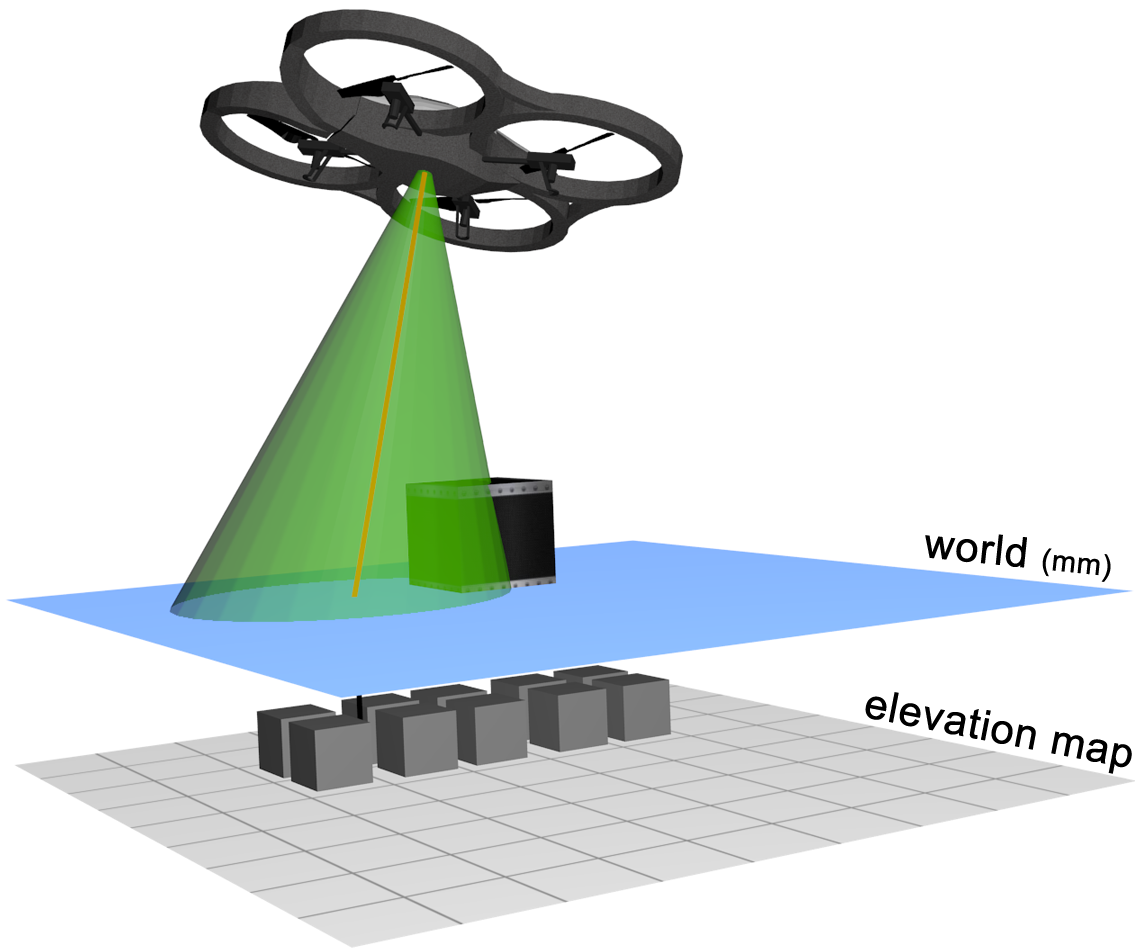
\includegraphics[width=0.4\linewidth]{images/elevation_map2.png}}
    \subfigure[Blup]{\label{visual-slam-elevation-map3}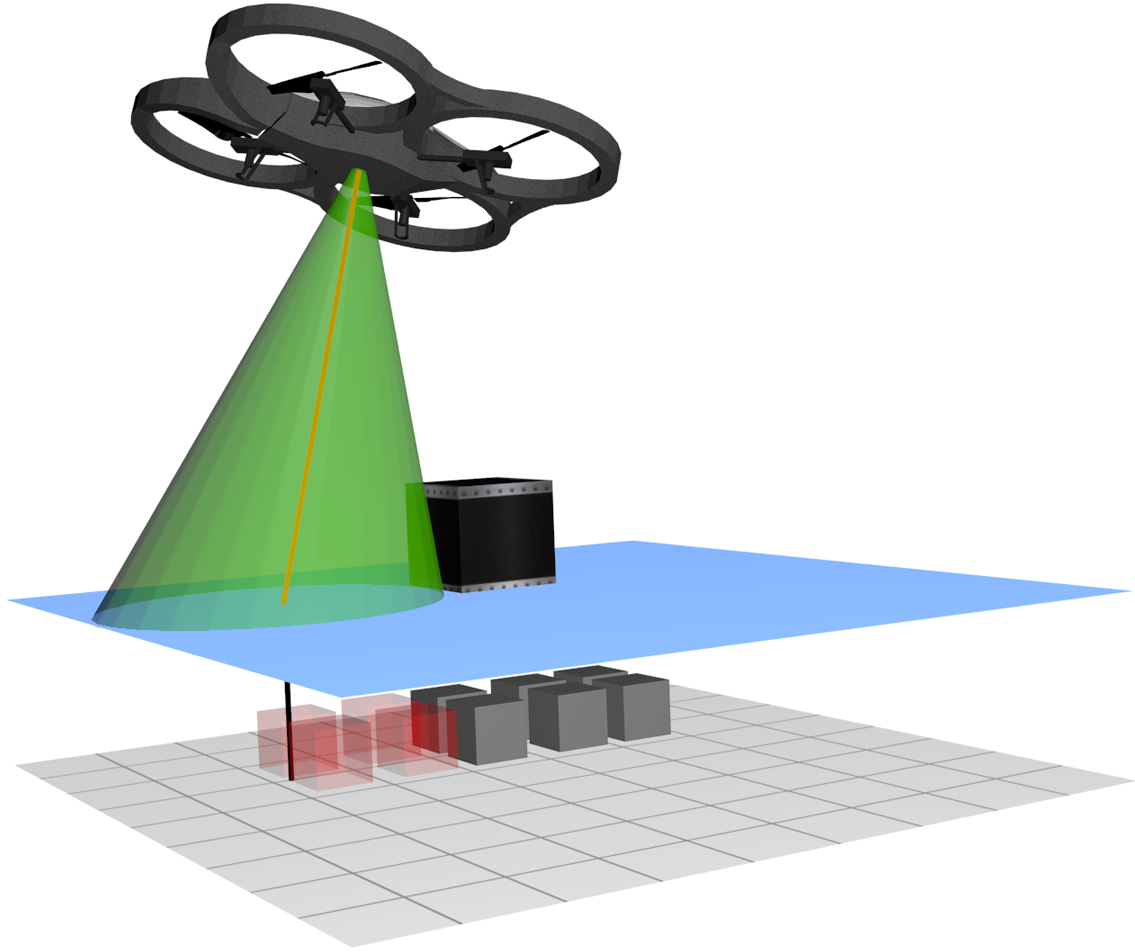
\includegraphics[width=0.4\linewidth]{images/elevation_map3.png}}
 \end{center}
  \caption{Blup.}
  \label{visual-slam-elevation-map}
\end{figure}



\chapter{Results}
\label{chapter:results}
In this chapter, the performance of both the simulation model and visual SLAM method are analyzed in a series of empirical experiments.
In Section \ref{sec:simulation_results}, the USARSim simulation model is validated.
A set of maneuvers is flown with the actual AR.Drone and
simulated AR.Drone. The differences between the maneuvers are studied in detail.
In Section \ref{sec:results-position-accuracy}, the accuracy of the estimated position is evaluated.
A set of 8-shapes is flown with the AR.Drone and the estimated positions are compared against the groundtruth from a laser range finder.
In Section \ref{sec:results-pose-recovery}, the proposed pose recovery approach is benchmarked against other pose recovery approaches.
In Section \ref{sec:res-cam-resolution}, the influence of the camera resolution is investigated.
Finally, in Section \ref{sec:results-elevation-accuracy} the accurracy of the elevation map is evaluated in terms of elevation error and the error in the estimated size of objects.


	\section{Simulation model}
\label{sec:simulation_results}
To evaluate the USARSim simulation model,  
a set of maneuvers is flown with the actual AR.Drone and
simulated AR.Drone. The differences between the maneuvers are studied in detail. To enable multiple repetitions of the same maneuver it is
described as a set of time points (milliseconds since initialization) each coupled to a movement command.
%We wrote wrappers for the AR.Drone programming interface and for USARSim interface which read these scripts and output a control
%signal, using the system clock to manage the timing independently from the game engine and the AR.Drone hardware.
Orientation, altitude and horizontal speed are recorded at a frequency of $200\hertz$ during the maneuvers. These are gathered through the AR.Drone's internal sensors and the onboard algorithms, which are
also used by the controller to operate the drone. The filtered output of the gyroscope is used
to estimate the orientation. The filtered output of the ultrasound distance sensor is used to estimate
the altitude. The onboard visual odometry algorithm is used to estimate the horizontal (linear
and lateral) speeds. The simulator has equivalent sensors. In addition, simulation can provide ground-truth data. 
Also for the real maneuvers an attempt was made to generate ground truth via an external reference system; the movements were recorded with a synchronized video system consisting of four firewire cameras, capturing images at 20 frames per second at a resolution of $1024 \times 768$ pixels. The position of the AR.Drone 
in each frame has been annotated by hand. 
%However, since the processing of the captured data is not yet complete, results from these trials are not presented in this paper.
%reference?!

Corresponding to NIST guidelines \cite{Jacoff2010STM}
a set of experiments of increasing complexity was performed. For the AR.Drone
four different experiments were designed.
The first experiment is a simple hover, in which the drone tries to maintain its position (both horizontal and vertical). The second experiment is linear movement, where the drone actuates a single movement command. The third experiment is a small horizontal square. The last experiment is a small vertical square.

\subsubsection{Hovering}

Quadrotors have hovering abilities just like a helicopter. The stability in maintaining a hover depends
on environmental factors (wind, underground, aerodynamic interactions) and control software.
%In \cite{Michael2010ra} a
%horizontal positioning error of no more than $2\small{cm}$ and a vertical error of less than $0.6\small{cm}$ are reported for
%a tightly optimized stiff controller. In practice, softer controllers are used which are more robust and can
%recover from larger disturbances. In \cite{How2008} a horizontal and vertical positioning error of no more than $10\small{cm}$ are %reported. 
If no noise model is explicitly added, the USARSim model performs a perfect hover; when no control signal is given the
horizontal speeds are zero and the altitude stays exactly the same.

For the AR.Drone, this is a good zero-order model. One of the commercial features of the AR.Drone is its ease of operation. As part of this feature it
maintains a stable hover when given no other commands, which is accomplished by a visual feedback loop.
%The hover is quite robust and in impromptu
%ad-hoc tests was able to recover from major attitude disturbances up to $\sim45^o$. However, in this section we
%are concerned with the hovering behavior with minor disturbances. 
So, the hovering experiment is performed  
indoors
with an underground chosen to have enough texture for the onboard visual odometry estimation algorithm.

As experiment the AR.Drone maintains a hover for 35 seconds. This experiment was repeated 10 times,
collecting 60.000 movement samples for a total of 350 seconds. Over all samples the mean absolute error in horizontal
velocity (the Euclidean norm of the velocity vector) is $0.0422\small{m/s}$ with a sample variance of $0.0012\small{m^2/s^2}$. From
the samples we obtain the distribution of the linear and lateral velocity components. 

From the velocity logs the position of the AR.Drone during the 35-second 
flight was calculated. 
%Figure \ref{fig:scatterplot} shows a scatterplot of positions over all flights.
The mean absolute error of the horizontal position is $0.0707\small{m}$ with a sample variance of $0.0012\small{m^2}$.

\begin{comment} % to save some space
\begin{figure}[htb]
\centering
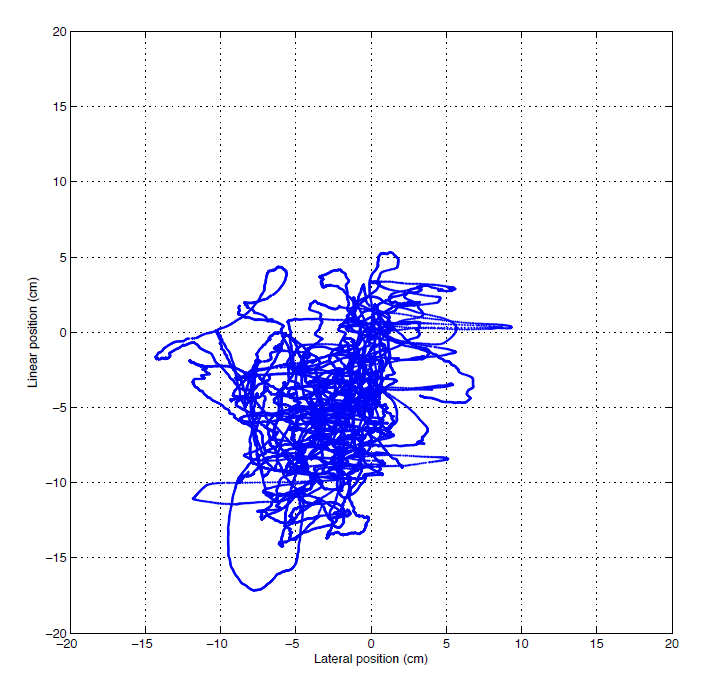
\includegraphics[width=8cm]{images/HoverScatterPlot.png}
\caption{Scatter plot of the horizontal position aggregated over all hover flights.}
\label{fig:scatterplot}
\end{figure}
\end{comment}

\subsubsection{Horizontal movement}

In this experiment the AR.Drone is flown in a straight line. It is given a control pulse (i.e., pitch) with a constant signal
for 5 different time periods: 0.1s, 1s, 2s, 3s, and 5s. Each pulse is followed by a null signal for enough time for the AR.Drone to make a full stop and a negative pulse of the same magnitude for the same period,
resulting in a back and forth movement. In Figure \ref{fig:RealResponse}
 the red line shows the control signal, the blue line the response (i.e., velocity) of the AR.Drone. The experiment was repeated for 5 different speeds.
The control signal $s$ specifies the pitch of the AR.Drone as a factor (between 0 and 1) of the maximum absolute tilt $\theta_{max}$, which was set to the default value\footnote{ARDrone firmware (1.3.3)}. % iPhone uses 12deg
The trials were performed with the
values of 0.05, 0.10, 0.15, 0.20, 0.25 for the control signal $s$.

\begin{figure}[htb]
\centering
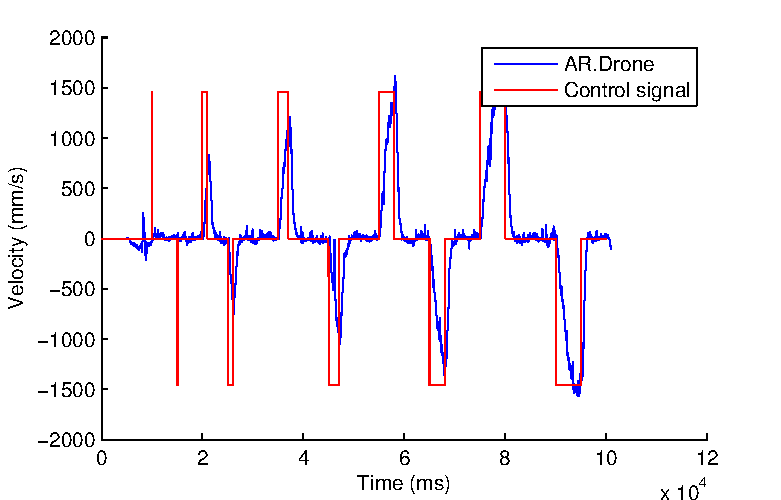
\includegraphics[width=11cm]{images/Dr7Ov-eps-converted-to.pdf}
\caption{Velocity of the real AR.Drone (blue) on a number of control pulses (red) with a pitch of $s=0.15 \times \theta_{max}$ .}
\label{fig:RealResponse}
\end{figure}

Robots in USARSim are controlled with a standardized interface, which uses SI units. A robot in USARSim expects a DRIVE command with a speed in $m/s$ and not the AR.Drone native signal $s$. 
Thus in order to 
fly comparable trials 
the relation between the AR.Drone's angle of attack $\alpha$ and the corresponding velocity $v$ has to be investigated.
When flying straight forward in no-wind conditions, the angle of attack $\alpha$ is equivalent with the pitch $\theta$.
In order to do this the samples from the logs where the AR.Drone has achieved maximum
velocity have to be selected. Closer inspection of the velocity logs show that in each trial there is still constant increase of velocity for the first three pulses. For the last two pulses there is obvious plateauing, which indicates that the last two seconds of the five-second pulses is a good indication for the maximum velocity. Therefore the velocity at those
last two seconds was used to compute mean absolute speeds $\bar{v}$, which are combined with the mean absolute
pitch $\bar{\theta}$ as measured by the MEMS gyroscope. The estimates for $\bar{v}$ and pitch $\bar{\theta}$ are presented in Table~\ref{tab:angle_of_attack} together with their standard deviation. 
% Looking at the values for the pitch we see that these differ from the expected angles listed above.
Extrapolating the mean pitch $\bar{\theta}\simeq7.5^o$ at 
control value $s=0.25$ to the maximum control signal gives an indication of
the AR.Drone's maximum pitch $\theta_{max}\simeq30^o$ value. For typical usage, the angle of attack never exceeds $12^o$ degrees.

\begin{table}[htb]    \centering
    \begin{tabular}
        { | l | l  l  l  l  l | }
        \hline 
          &  \multicolumn{5}{| l |}{Control signal $s$} \\
          & 0.05 & 0.10 & 0.15 & 0.20 & 0.25 \\    
        \hline
        $\bar{v}$ (m/s) & 0.4044 & 0.6284 & 1.4427 & 1.7587 & 2.2094 \\
        $\sigma_v$ (m/s) & 0.096 & 0.226 & 0.070 & 0.126 & 0.165 \\
        \hline
        $\bar{\theta}$ (deg) & 1.4654 & 2.9025 & 4.1227 & 5.7457 & 7.4496 \\
        $\sigma_\theta$ (deg) & 0.455 & 0.593 & 0.482 & 0.552 & 0.921 \\
        \hline
    \end{tabular}    \caption{Averaged velocity $\bar{v}$ measured at the end of a 5 seconds pulse of the control signal $s$, including the corresponding pitch $\bar{\theta}$ as measured by the gyroscope.}
    \label{tab:angle_of_attack}
\end{table}

\begin{comment}
\begin{table}[htb]    \centering
    \begin{tabular} 
        { | l | l | l | l | l | l | }
        \hline 
          &  \multicolumn{5}{|l|}{Control signal $s$} \\
          & 0.05 & 0.10 & 0.15 & 0.20 & 0.25 \\
        \hline
        $\bar{v}$ (m/s) & 0.4044 & 0.6284 & 1.4427 & 1.7587 & 2.2094 \\
        $\sigma_v$ (m/s) & 0.096 & 0.226 & 0.070 & 0.126 & 0.165 \\
        \hline
        $\bar{\theta}$ (deg) & 1.4654 & 2.9025 & 4.1227 & 5.7457 & 7.4496 \\
        $\sigma_\theta$ (deg) & 0.455 & 0.593 & 0.482 & 0.552 & 0.921 \\
        \hline
    \end{tabular}    \caption{Averaged velocity $\bar{v}$ measured at the end of a 5 seconds pulse of the control signal $s$, including the corresponding pitch 
$\bar{\theta}$ as measured by the IMU.} 
    \label{tab:angle_of_attack}
\end{table}
\end{comment}

To convert the AR.Drone's control signal $s$ to USARSim commands $v$ a least-squares fit through the points of Table~\ref{tab:angle_of_attack} is made for the linear function
$v = c \cdot \theta$, which gives us $c=0.2967$. 
Equation \ref{eq:conversion} gives the final conversion of a control signal $s$ to a velocity $v$ in $m/s$ given the
AR.Drone's maximum pitch $\theta_{max}$ in degrees.

\begin{equation}
v = 0.2967 \cdot s \cdot \theta_{max}
\label{eq:conversion}
\end{equation}

The USARSim model has a parameter $P_\theta$ for calculating the angle (radian) given the velocity, which
% we can calculate from the coefficient $c$ above by converting from degrees to radians. This gives us the
% theoretical $P_\theta = \frac{1}{0.2967} \cdot \frac{\pi}{180} = 0.0588$. However, doing a least-squares fit on the angle given the velocity gives 
is the value $\hat{P}_\theta = 0.057$, as used in subsequent simulations.

The next experiment checks the acceleration of the real and simulated AR.Drone. First we give an estimate of how quickly the AR.Drone's controller changes its pitch to match the commanded pitch and how well it can keep it. For this we select all samples from 100ms after the start
of the 2s, 3s and 5s pulses till the first sample at which the commanded pitch has been reached. This
corresponds to the time-span between which the AR.Drone has started to act on the change in the control
signal until it reaches the commanded pitch. The result is illustrated in Figure \ref{fig:ComparisonOfResponse}.
%For each of these spans we estimate the tangent:

\begin{figure}[htb]
\centering
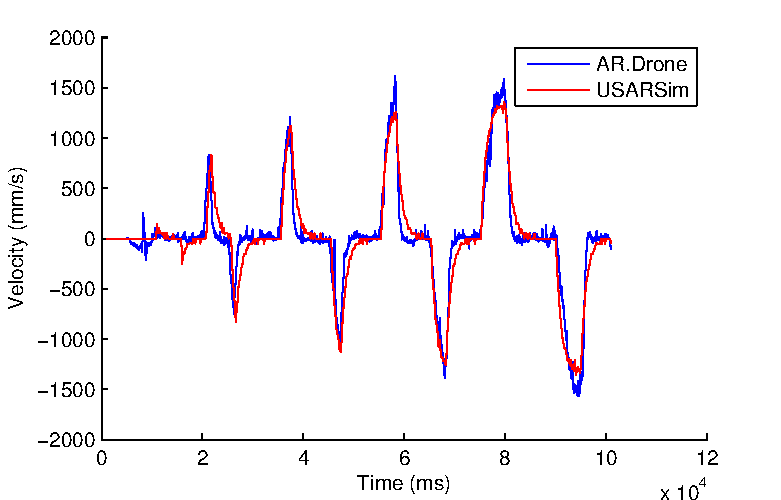
\includegraphics[width=11cm]{images/RYtdB-eps-converted-to.pdf}
\caption{Velocity of the real (blue) and simulated AR.Drone (red) on the same control pulses as shown in Figure~\ref{fig:RealResponse}.}

\label{fig:ComparisonOfResponse}
\end{figure}

As one can see, the acceleration has for the real and simulated AR.Drone nearly the same slope. The deceleration of the simulated AR.Drone is slightly lower. In the real AR.Drone the feedback loop (based on the onboard visual odometry of the ground camera) actively decelerates the system. Overall, the dynamic behavior of the simulator closely resembles the dynamic behavior of the real system. Additionally, tests with more complex maneuvers (horizontal and vertical square) have been recorded, but unfortunately not yet analyzed in detail.




\section{Position accuracy}
\label{sec:results-position-accuracy}
An experiment has been carried out to evaluate the accuracy of the AR.Drone's estimated position.
This experiment is performed above a texture-rich floor (Section \ref{sec:exp1-texture-poor}), a texture-poor floor (Section \ref{sec:exp1-texture-poor}) and a floor that resembles the circumstances encountered during the IMAV competitions.
The position can be estimated using different methods and the accuracy of all these methods are evaluated.
To ensure fair comparison of the different estimation methods, a flight was recorded (Section \ref{sec:proposed-framework}) and played back to generate the same input for all methods.

The first position estimation method integrates the AR.Drone's onboard velocity (AV) measurements to estimate the position (Section \ref{sec:pose_estimation}).
Recent AR.Drone firmwares calculcate an estimated position onboard\footnote{Firmware 1.7.4}, which is used as second estimation method.
The third position estimation method uses the visual odometry method presented in this thesis (Section \ref{sec:visual-slam-visual-odemetry}).
The final estimation method uses the AR.Drone's onboard velocity (AV) for frequent position updates and the presented localization method (Section \ref{sec:localization}) to localize against the map that is constructed during flight.

The estimated position is compared against the groundtruth (real) position to calculcate the accuracy of the estimated position.
Great care was taken to collect accurate groundtruth of the AR.Drone's position.
A high-end laser range finder (LRF)\footnote{Hokuyo UTM-30LX, \url{http://www.hokuyo-aut.jp/02sensor/07scanner/utm_30lx.html}} is used to determine the position of the AR.Drone.
The LRF measures distance to objects.
A window is placed on the measurements to filter out measurements that originate from the environment.
All remaining distance measurements are assumed to originate from the AR.Drone.
The mean position of the filtered distance measurements is used as center position of the AR.Drone.
Futhermore, a white cylinder with a diameter of 9\begin{small}cm\end{small} and a height of 37\begin{small}cm\end{small} was added on top of the AR.Drone to improve its visability for the LRF.

\begin{figure}[htb]
\centering
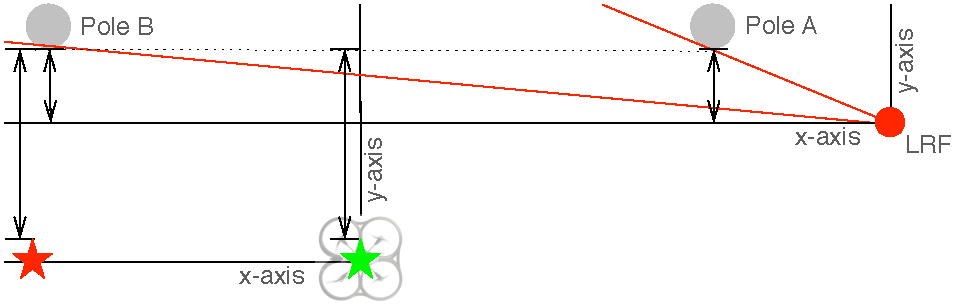
\includegraphics[width=13cm]{images/exp1-floorplan-align.pdf}
\caption{The alignment of the laser range finder and the AR.Drone. The laser range finder (LRF) is aligned against two poles. The takeoff position is marked with a green star. The red star indicates the marked heading direction of the AR.Drone. A laser pointer is used to align the heading direction of the AR.Drone to the marker position.}
\label{fig:exp1-floorplan-align}
\end{figure}

The LRF measures the AR.Drone's position in its own reference frame.
Therefore, the AR.Drone's reference frame has to be accurately aligned with the LRF's reference frame.
This is achieved by rotating the AR.Drone before takeoff, such that it points in exactly the same direction as the LRF.
The following method was used to align the LRF and the AR.Drone (Figure \ref{fig:exp1-floorplan-align}).
First, the LRF is aligned against two poles in the environment.
The LRF is rotated until both poles obtained an equal y-distance in the LRF's reference frame.
Now, the LRF's x-axis is parallel to the poles.
Next, the AR.Drone's takeoff position and orientation are determined.
The takeoff position is marked on the floor (green star).
Another position was marked (red star) to indicate the desired heading direction of the AR.Drone.
Both marked position are parallel to the LRF's x-axis and the two poles.
Finally, a laser pointer is used to align the heading direction of the AR.Drone to the marked position.





\subsection{Texture-rich floor}
\label{sec:exp1-texture-rich}
The first experiment was performed above a texture-rich floor (Figure \ref{fig:exp1-floor}), to benchmark the methods in preferable circumstances.
Magazine were spraid out on the floor to provide sufficient texture for the computer vision algorithms.
The AR.Drone flew three 8-shapes above the magazines.
An 8-shape was chosen to capture an intermediate loop.

\begin{figure}[htb!]
\centering
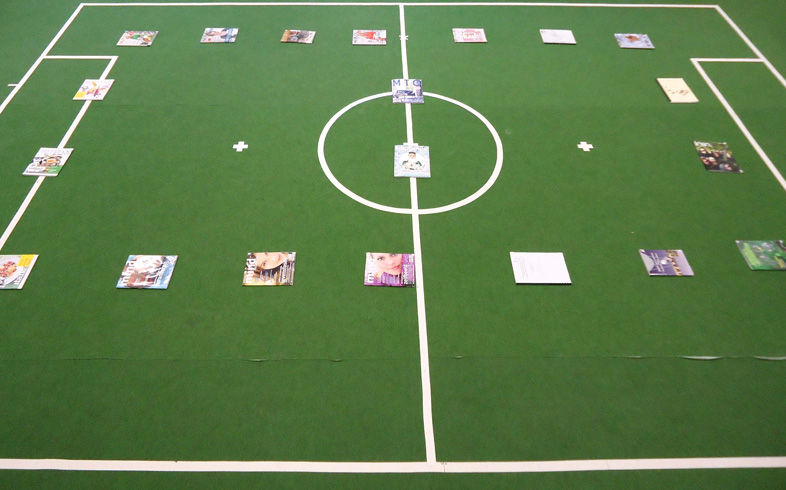
\includegraphics[width=8cm]{images/exp1-floor.jpg}
\caption{Photo of the texture-rich floor used for the first experiment. Magazine are spraid out on the floor to provide sufficient texture. The dimensions of the 8-shape are approximately $5\small{m} \times 2.5\small{m}$.}
\label{fig:exp1-floor}
\end{figure}

\begin{table}[htb!]
    \centering
    \begin{tabular}
        { | l | l | l | } 
	\hline
	Method & Mean absolute error (\small{mm}) & Mean relative error (percentage of trajectory length) \\
        \hline
        onboard velocity (AV) & 477 & 0.715\% \\
	onboard position (AP) & 476 & 0.714\% \\
	visual odometry (VO) & 552 & 0.828\% \\
	AV + localization & 260 & 0.390\% \\
	\hline
    \end{tabular}
    \caption{Errors made by the position estimation methods when flying above a texture-rich floor.}
    \label{tab:res_mapping}
\end{table}

\begin{figure}[htb!]
\centering
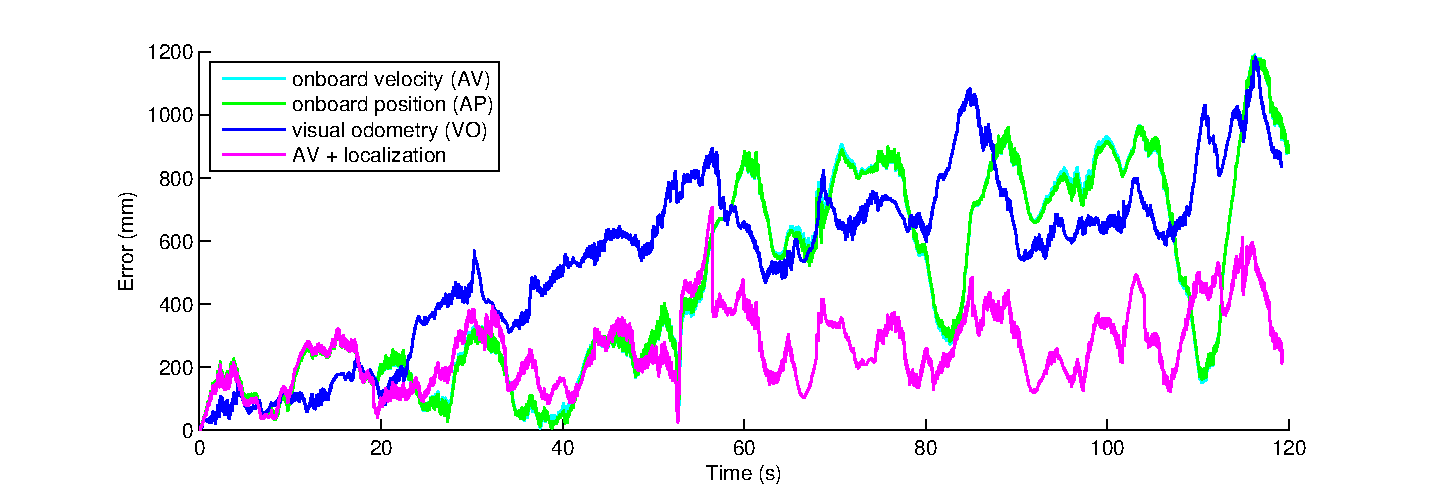
\includegraphics[width=\linewidth]{images/exp1-run13-error.eps}
\caption{Errors between the estimated positions and the groundtruth.}
\label{fig:exp1-texture-error}
\end{figure}

\begin{figure}[htb!]
\centering
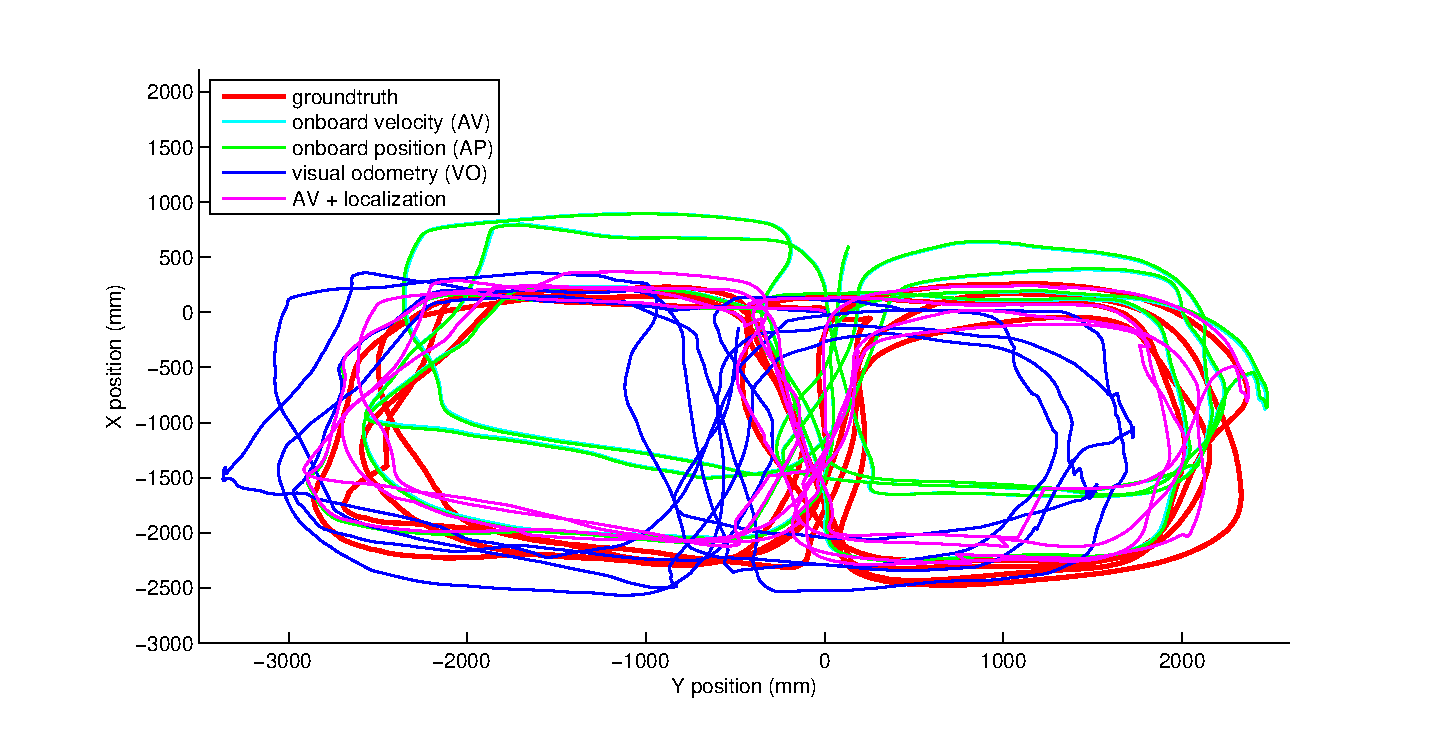
\includegraphics[width=\linewidth]{images/exp1-run13-path.eps}
\caption{Estimated trajectories of the different position estimation methods. The AR.Drone flew three 8-shapes above above a texture-rich floor.}
\label{fig:exp1-texture-path}
\end{figure}

\begin{figure}[htb!]
\centering
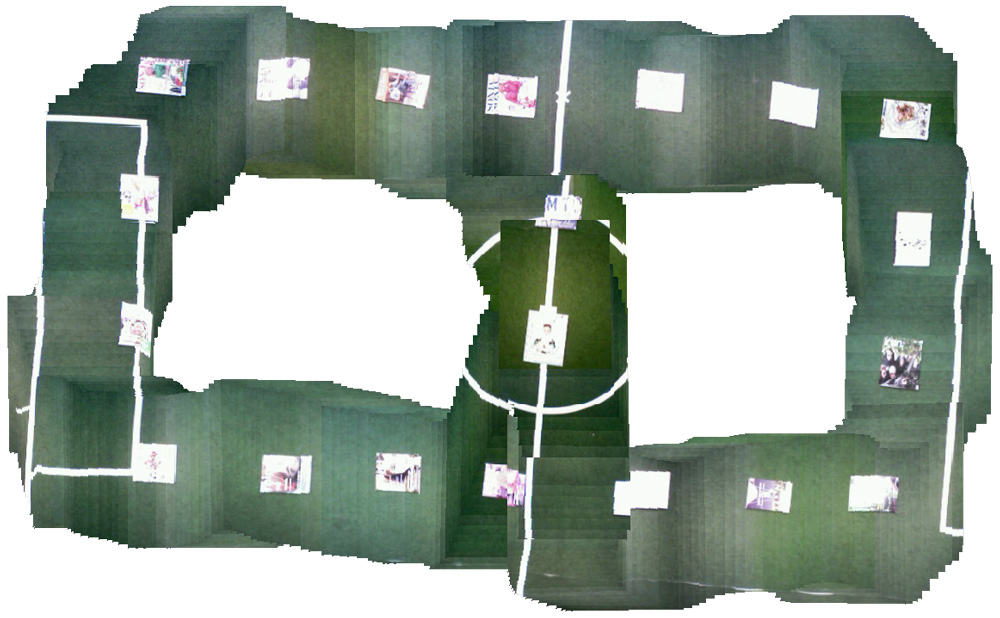
\includegraphics[width=0.75\linewidth]{images/exp1-run13-map.jpg}
\caption{Visual map created by the visual mapping method (Section \ref{sec:texture_map}). The map is constructed during the first 8-shape. The position estimates are based on the onboard velocity (AV) and the visual localization method (Section \ref{sec:localization}).}
\label{fig:exp1-texture-map}
\end{figure}

The results of this experiment can be found in Table \ref{tab:res_mapping} and Figures \ref{fig:exp1-texture-error} (errors), \ref{fig:exp1-texture-path} (trajectories) and \ref{fig:exp1-texture-map} (visual map).
For the encountered circumstances, all methods are able to estimate the position quite accurately.
Both the onboard velocity (AV) method and the onboard position (AP) method produce exactly the same trajectory, which implies the onboard position estimate (AP) is based on the velocity that is estimated by the AR.Drone.

The onboard velocity (AV) slightly outperforms the visual odometry (VO) method presented in Section \ref{sec:visual-slam-visual-odemetry}.
An explanation could be that the AR.Drone features an additional optical flow algorithm that is used when the appearance-based method is performing poorly.
From Figure \ref{fig:exp1-texture-path} can be seen that the onboard velocity (AV) method has the largest error in the x-direction.
Around $54\begin{small}s\end{small}$ the error is increasing rapidly.
Analysis of the dataset pointed out that a small part of a magazine and a large part of a white line were in range of the camera.
This resulted in a velocity thas was estimated in the wrong direction along the white line, which can be recognized by the small green loop on the right side of Figure \ref{fig:exp1-texture-path}.

The visual odometry (VO) method has the largest error in the y-direction.
Around $80\begin{small}s\end{small}$ the error is increasing rapidly.
Analysis of the dataset pointed out that the magazines were out of the camera's range. During this period the velocities could not be updated.

A combination of the onboard velocity (AV) with localization against the map outperforms all other methods.
With localization against the map, the error is reduced significantly.
%The map is constructed during the first 8-shape (first $40\begin{small}s\end{small}$).
From Figure \ref{fig:exp1-texture-error} can be seen that the maximum error is not exceeding the error made during the first 8-shape.
The repetitive error pattern suggests that the error of the estimated position largely depends on the quality (accuracy) of the map, if localization can be performed regularly.
%Around $85\begin{small}s\end{small}$ the error increases rapidly. This error is caused by a false match %against the map. However, future localizations correct this mistake.

The visual map (Figure \ref{fig:exp1-texture-map}) shows that the AR.Drone's onboard white balancing is reducing the contrast of the magazines, which affects the performance of the feature detector.
This is a source of error for the visual odometry (VO) algorithm.
Futhermore, errors in the ultrasound and IMU measurements are other sources that result in errors in the estimated velocities.

% 66674 mm






\subsection{Texture-poor floor}
\label{sec:exp1-texture-poor}
The experiment is repeated above a floor with low texture, to benchmark the methods in difficult circumstances.
Therefore, all magazines (Figure \ref{fig:exp1-floor}) are removed, resulting in a green floor with few white lines.
The AR.Drone flew a single 8-shape.


% 19616
\begin{table}[htb!]
    \centering
    \begin{tabular}
        { | l | l | l | } 
	\hline
	Method & Mean absolute error (\small{mm}) & Mean relative error (percentage of trajectory length) \\
        \hline
        onboard velocity (AV) & 1292 & 6.586\% \\
	onboard position (AP) & 1294 & 6.597\% \\
	visual odometry (VO) & 1126 & 5.740\% \\
	\hline
    \end{tabular}
    \caption{Errors made by the position estimation methods when flying above a texture-poor floor.}
    \label{tab:res_mapping-poor}
\end{table}

\begin{figure}[htb!]
\centering
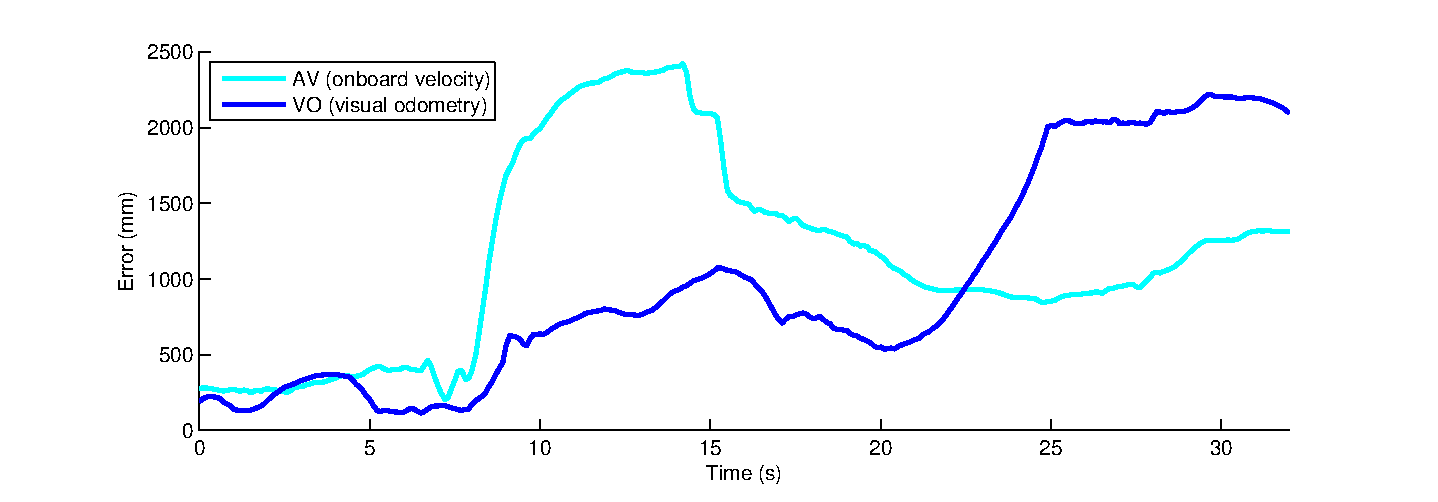
\includegraphics[width=\linewidth]{images/exp1-run2-error.eps}
\caption{Errors made by the position estimation methods when flying above a texture-poor floor.}
\label{fig:exp1-notexture-error}
\end{figure}

\begin{figure}[htb!]
\centering
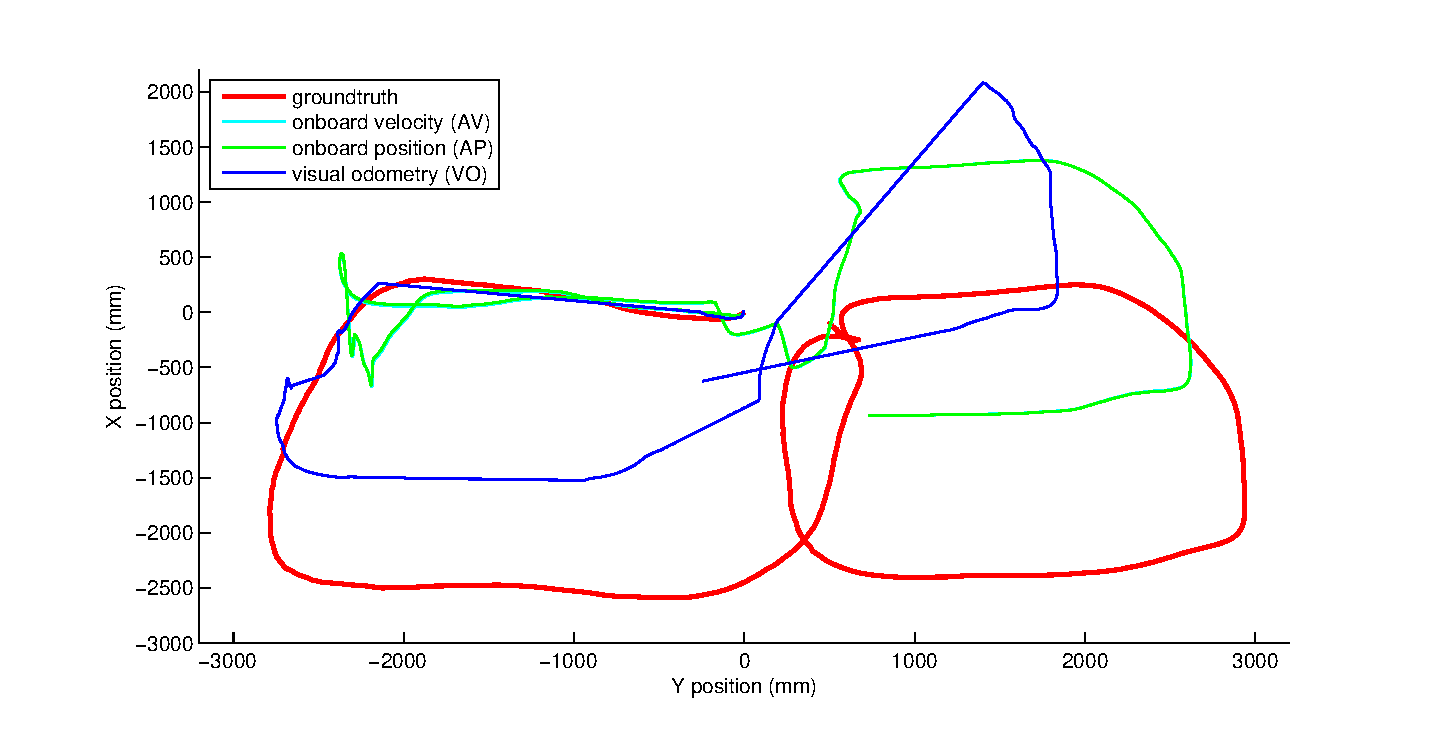
\includegraphics[width=\linewidth]{images/exp1-run2-path.eps}
\caption{Estimated trajectories of the different position estimation methods. The AR.Drone flew three 8-shapes above above a texture-poor floor.}
\label{fig:exp1-notexture-path}
\end{figure}

\begin{figure}[htb!]
\centering
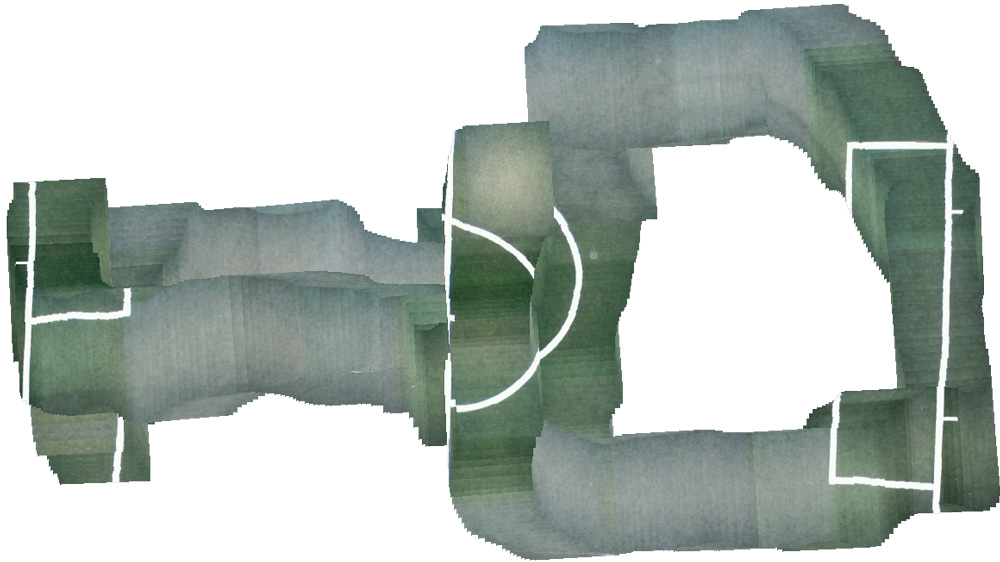
\includegraphics[width=0.75\linewidth]{images/exp1-run2-map.jpg}
\caption{Visual map created by the visual mapping method (Section \ref{sec:texture_map}). The position estimates are based on the onboard velocity (AV).}
\label{fig:exp1-notexture-map}
\end{figure}


The results of this experiment can be found in Table \ref{tab:res_mapping-poor} and Figures \ref{fig:exp1-notexture-error} (errors), \ref{fig:exp1-notexture-path} (trajectories) and \ref{fig:exp1-notexture-map} (visual map).
For the encountered circumstances, all methods are unable to estimate the position accurately.
Again, both the onboard velocity (AV) method and the onboard position (AP) method produce exactly the same trajectory.
Localization was not possible and therefore omitted from the plots.

The visual odometry (VO) method slightly outperforms the onboard velocity (AV) method.
One would expect that the AR.Drone's additional optical flow method outperforms appearance-based methods.
From Figure \ref{fig:exp1-notexture-path} can be seen that the onboard velocity (AV) method fails to correctly deal with the lines on the floor.
The onboard velocity (AV) methods measures a velocity in the wrong direction along the lines, resulting in a large error.
One would expect that the onboard aerodynamic model should correct this (i.e., the angle of the AR.Drone can be used to determine the correct direction).

From Figure \ref{fig:exp1-notexture-path} can be seen that the visual odometry (VO) method underestimates the velocities.
At places where the AR.Drone changes direction, the method was able to track sufficient features (due to the presence of corners) and estimate the velocities.
At these places, the AR.Drone's velocity was below the average speed due to deaccelerations.
Along most straight parts of the trajectory insufficient features were tracked and the (higher) velocity could not be updated.
Therefore, the lower velocities during the direction changes are maintained when flying along the straight parts of the trajectory.





\subsection{IMAV circumstances}
\label{sec:exp1-imav-circumstances}
The experiment is repeated in a sports hall, to benchmark the methods in circumstances encountered during the IMAV competitions.
This environment closely resembles the environment of the IMAV2011 indoor competitions.
The trajectory of the AR.Drone is increased to approximately $12 \times 2.5\small{m}$ in order to match the trajectory of the IMAV competitions.
This  trajectory is flown three times.
%The AR.Drone flown three 8-shapes.
Furthermore, the flight altitude of the AR.Drone is increased to $2\begin{small}m\end{small}$.
This allows the camera to capture sufficient visual clues (i.e., lines) to perform for visual odometry.




\clearpage
\section{Accuracy w.r.t. pose recovery approaches}
\label{sec:results-pose-recovery}
Section \ref{sec:pose-recovery} proposed a novel method to robustly recover the translation and rotation between \textit{two frames} (visual odometry) or \textit{a frame and a map} (localization).
Instead of computing a full perspective, affine or Euclidean transformation, a more pragmatic approach is used.
In this experiment, the proposed pose recovery approach is benchmarked against other pose recovery approaches.

An approach similar to the position accuracy experiment from Section \ref{sec:results-position-accuracy} is used.
The positions are estimated using the Visual Odometry (VO) method from Section \ref{sec:visual-slam-visual-odemetry}, which relies on pose recovery to determine the velocity.
The recorded dataset of the texture-rich floor (Section \ref{sec:exp1-texture-rich} ) is used as input.
 
The pose recovery approaches is benchmarked against OpenCV's robust \textit{Euclidean transformation}, \textit{affine transformation} and \textit{perspective transformation}.
The \textbf{Euclidean transformation} is computed using OpenCV's \textit{estimateRigidTransform}\footnote{\url{http://opencv.itseez.com/modules/video/doc/motion_analysis_and_object_tracking.html?highlight=estimateRigidTransform}} with the parameter \textit{fullAffine} off to compute a Euclidean transformation.
The translation vector from the transformation matrix is used as velocity estimate.
The maximum allowed reprojection error is set to $10\small{mm}$.
Additional filtering is required to remove bad transformation.
A recovered transformation is rejected if the percentage of inliers is below $50\%$ or if the translation is too large ($T \geq 500\small{mm}$).
The \textbf{affine transformation} is computed using OpenCV's \textit{estimateRigidTransform}\footnote{\url{http://opencv.itseez.com/modules/video/doc/motion_analysis_and_object_tracking.html?highlight=estimateRigidTransform}} with the parameter \textit{fullAffine} on.
The \textbf{perspective transformation} is computed using OpenCV's \textit{findHomography}\footnote{\url{http://opencv.itseez.com/modules/video/doc/motion_analysis_and_object_tracking.html?highlight=findhomography}} with a RANSAC-based robust method.
The translation vector from the homography is used as velocity estimate.

\begin{table}[htb!]
    \centering
    \begin{tabular}
        { | l | l | l | } 
	\hline
	Method & Mean absolute error (\small{mm}) & \parbox{5cm}{Mean relative error \\(percentage of trajectory length)} \\
        \hline
        visual odometry (VO) & 552 & 0.828\% \\
	visual odometry (VO) - euclidean transform & 967 & 1.449\% \\
	visual odometry (VO) - affine transform & 3784 & 5.672\% \\
	visual odometry (VO) - perspective transform & 8923 & 13.375\% \\
	\hline
    \end{tabular}
    \caption{Errors made by the visual odometry (VO) position estimation method when using different pose recovery approaches.}
    \label{tab:res_transform}
\end{table}

The results of this experiment can be found in Table \ref{tab:res_transform} and Figure \ref{fig:exp4-transform-error}.
The proposed pose recovery approach outperforms the other pose recovery approaches.
This approach reduces the degrees of freedom and is more robust against noise.
This corresponds with the observations made by Caballero et al (Section \ref{related-online-mosaicking}).
OpenCV's pose recovery approaches use the percentage of inliers to determine the quality of a recovered pose.
However, the percentage of inliers may not reflect the actual quality of a recovered pose.
For example, a faulty transformation (pose) can maximize the number of inliers, as described in Section \ref{sec:pose-recovery}.
The proposed approach uses the covariance between the points of a hypothesis to determine the quality of a recovered pose.
This approach is able to estimate the quality of a recovered pose more accurately, resulting in recovered poses that contain less error.
%This seems to be a beter measure to determine the quality, resulting in a reduced error.


\begin{figure}[htb!]
\centering
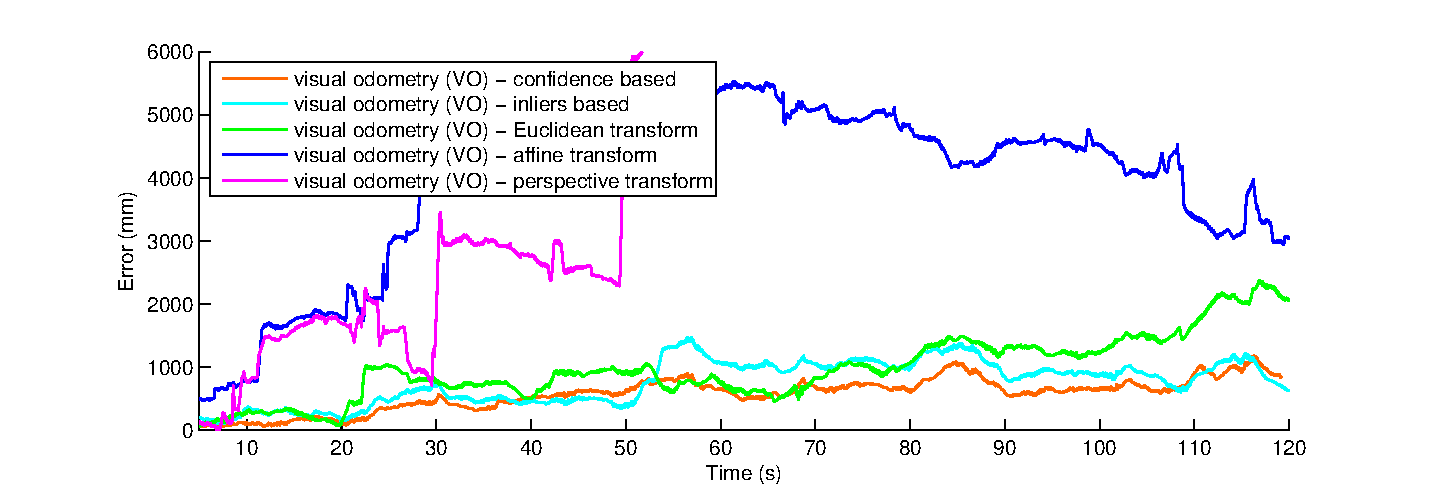
\includegraphics[width=\linewidth]{images/exp4-transform-error.eps}
\caption{Errors between the estimated positions and the groundtruth.}
\label{fig:exp4-transform-error}
\end{figure}



\clearpage
\section{Accuracy w.r.t. camera resolution}
\label{sec:res-cam-resolution}
The AR.Drone is equipped with a low resolution down-looking camera.
The recent developments in miniaturing high-resolution cameras enables MAVs to be equipped with high-resolution cameras.
This poses the question if the proposed method benefit from an increased image resolution.

In this experiment, the accuracy of the estimated position is evaluated for various camera resolutions.
An approach similar to the position accuracy experiment from Section \ref{sec:results-position-accuracy} is used.
The positions are estimated using the Visual Odometry (VO) method from Section \ref{sec:visual-slam-visual-odemetry}.
The recorded dataset of the texture-rich floor (Section \ref{sec:exp1-texture-rich} ) is used as input.
The experiment is repeated for different camera resolutions, which are simulated by downscaling the original camera images.
%The recorded images are downscaled to $90\%$, $66.6\%$ and $33.3\%$ of the AR.Drone's resolution.
The camera calibration matrix is scaled accordingly.

The experiment is repeated with a simulated AR.Drone in USARSim, which enables to both increase and decrease the resolution of the camera.
Care was taken to mimic the AR.Drone's camera\footnote{A previous article \cite{Visser2011imav} describes the influence of white balancing on image stitching and how to mimic the real images as close as possible.}.

The results of the real AR.Drone can be found in Table \ref{tab:res-resolution-ar} and the results of the simulated AR.Drone can be found in Table \ref{tab:res-resolution-usar}.
For each camera resolution, the number of processed frames is counted.
Not all frames can be (accurately) related to its previous frame to determine (extract) the velocity, which is indicated by the third column.
The fourth column describes the mean error of the estimated positions.
In Figure \ref{fig:exp3-error2}, the relation between image resolution and accuracy of the estimated position is plotted.
In Figure \ref{fig:exp3-error}, the position error is plotted over time.


\begin{table}[htb!]
    \centering
    \begin{tabular}
        { | l | l | l | l | } 
	\hline
	Resolution & Nr. frames processed & Nr. frames velocity extracted & Mean error (mm) \\
        \hline
        33.3\% & 2275 & 213 & 11742 \\
	66.6\% & 2239 & 1346 & 2166 \\
	90.0\% & 2259 & 1847 & \textbf{531} \\
	100.0\% & 2168 & 1945 & 579 \\
	\hline
    \end{tabular}
    \caption{Real AR.Drone. Mean error of the estimation position for different camera resolutions. For each camera resolution, the number of processed frames is counted. A part of these frames can be used to extract the velocity of the AR.Drone.}
    \label{tab:res-resolution-ar}
\end{table}

\begin{table}[htb!]
    \centering
    \begin{tabular}
        { | l | l | l | l | } 
	\hline
	Resolution & Nr. frames processed & Nr. frames velocity extracted & Mean error (mm) \\
        \hline
        33.3\% & 1600 & 5 & 9295 \\
	66.6\% & 1598 & 247 & 528 \\
	90.0\% & 1570 & 850 & 100 \\
	100.0\% & 1365 & 841 & \textbf{73} \\
	133.3\% & 1000 & 791 & 100 \\
	166.6\% & 685 & 612 & 77 \\
	200.0\% & 552 & 531 & 98 \\
	\hline
    \end{tabular}
    \caption{Simulated AR.Drone (USARSim). Mean error of the estimation position for different camera resolutions. For each camera resolution, the number of processed frames is counted. A part of these frames can be used to extract the velocity of the AR.Drone.}
    \label{tab:res-resolution-usar}
\end{table}


\begin{figure}[htb!]
  \begin{center}
    \subfigure[Real AR.Drone]{\label{fig:exp3-2-a}%
	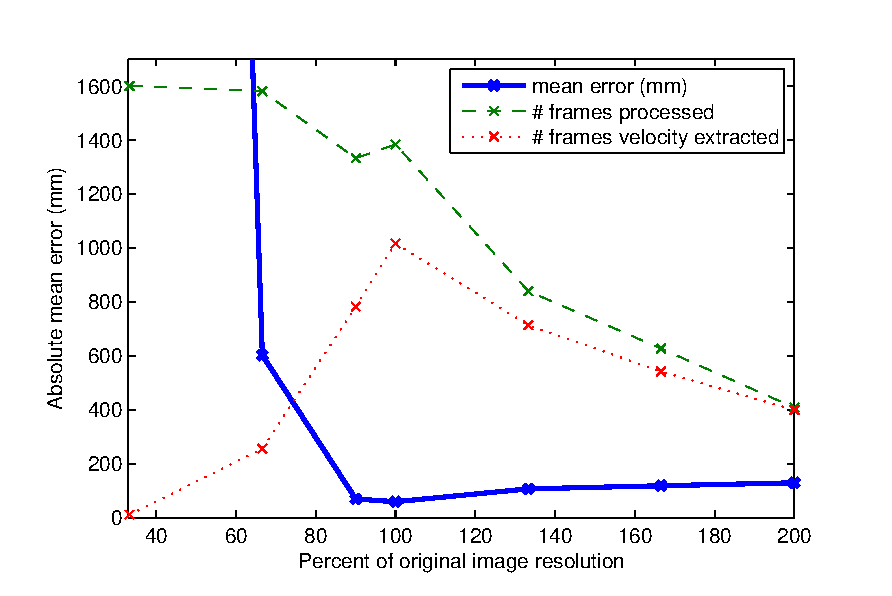
\includegraphics[width=0.55\linewidth]{images/exp3-ar-res-error2.eps}}%
    \subfigure[Simulated AR.Drone (USARSim)]{\label{fig:exp3-2-b}%
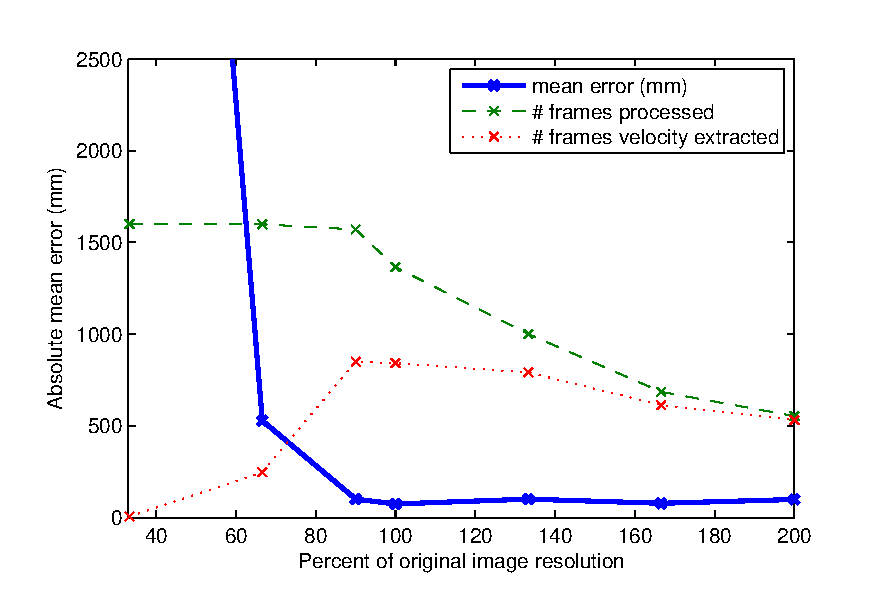
\includegraphics[width=0.55\linewidth]{images/exp3-usar-res-error2.eps}}

 \end{center}
  \caption{Mean error of the estimated position with respect to the image resolution. For each resolution, the number of processed frames is counted (green line). A part of these frames can be used to extract the velocity of the AR.Drone (red line).}
  \label{fig:exp3-error2}
\end{figure}


From Table \ref{tab:res-resolution-ar} can be seen that the original camera resolution is sufficient for frequent velocity updates.
Out of the $2168$ processes frames, $1945$ frames ($90\%$) could be used to extract the velocity using the Visual Odometry method.
When the image resolution is slightly decreased to $90\%$ of the original resolution, more frames were processed.
Algorithm such as the SURF feature extractor require less processing time, allowing more frames to be processed.
However, only $82\%$ of these frames could be used to extract the velocity.
When the resolution decreases further, the number of processed frames remains stable, which indicates the processing time is not significantly decreasing.
However, the number of frames that could be used to extract the velocity is decreasing.
This indicates that the camera images with lower resolution are less usefull for the Visual Odometry method.
This is reflected by the mean error of the different camera resolutions.
In general, a lower camera resolution results in a larger error in the estimated position (Figure \ref{fig:exp3-2-a}).
An exception is the camera resolution of $90\%$, which has a slightly lower error than the original resolution.
This exception is probably caused by a coincidental drift that reduces the error.

The results of the simulated AR.Drone can be found in Table \ref{tab:res-resolution-usar} and Figure \ref{fig:exp3-2-b}.
The overall mean errors are smaller than the real AR.Drone, due to the lack of noise generated by the IMU and ultrasound sensor.
Similar to the real AR.Drone, a reduced resolution results in more frames being processed, but less frames that could be used to extract the velocity.
When the resolution increases, the number of processed frames decreases due to the increased computational time per frame.
However, the percentage of frames that could be used to extract the velocity increases.
This indicates that the camera images with a higher resolution are more usefull for the Visual Odometry method.
For the original resolution, $62\%$ of the processed frames could be used to extract the velocity. When the resolution is doubled, $96\%$ of the frames could be used to extract the velocity.
One would expect that an increased image resolution would result in a smaller error.
However, due to the increased computational time per frame, less frames can be processed resulting in less frequent velocity estimates.
This results in a mean error that is not smaller than the original resolution.

Based on these observations can be concluded that the AR.Drone's bottom camera resolution offers a good balance between image quality (usefulness) and processing time.
An increased camera resolution is expected to yield improved position accuracy when the machine running the SLAM method is able to maintain the number of processed frames when the image resolution increases.




\begin{figure}[htb!]
  \begin{center}
    \subfigure[Real AR.Drone]{\label{fig:exp3-a}%
	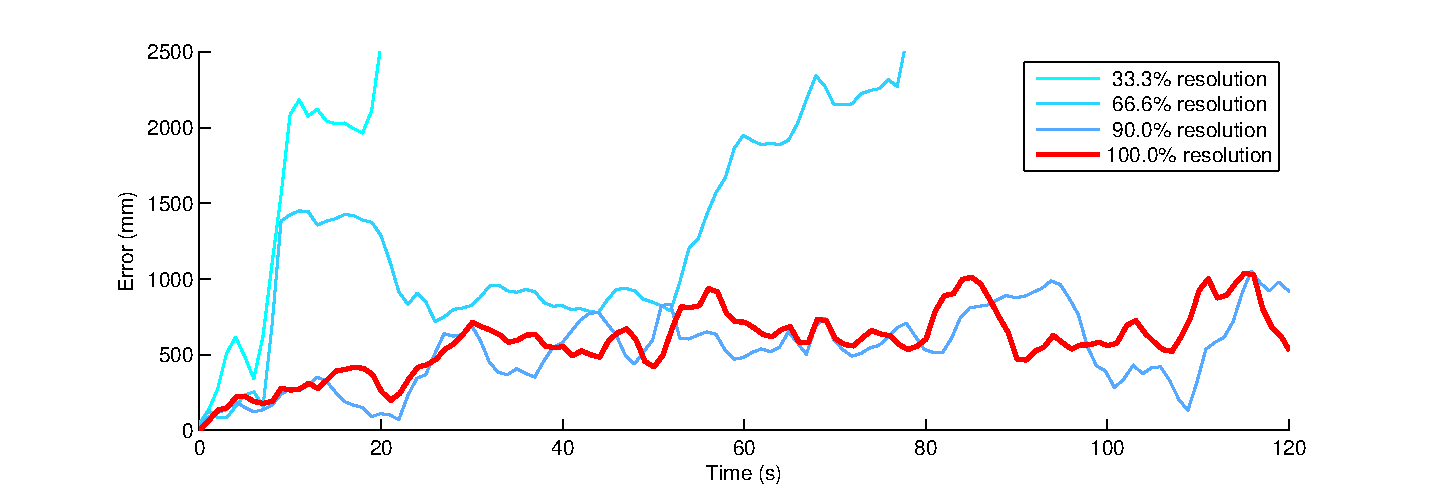
\includegraphics[width=0.85\linewidth]{images/exp3-ar-res-error.eps}}%
\\
    \subfigure[Simulated AR.Drone (USARSim)]{\label{fig:exp3-b}%
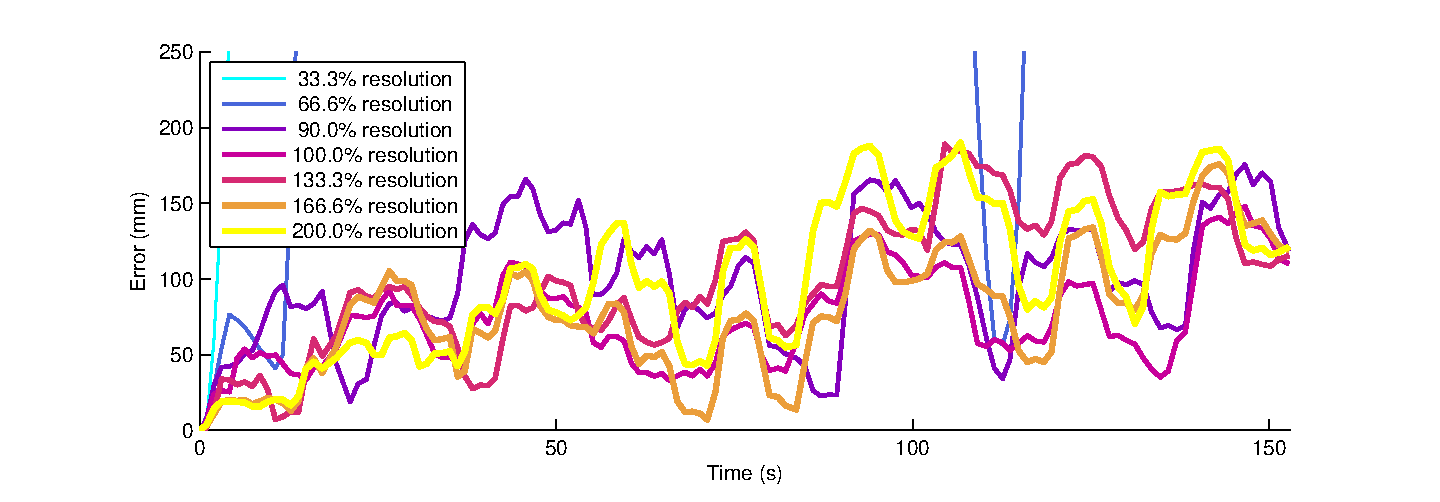
\includegraphics[width=0.85\linewidth]{images/exp3-usar-res-error.eps}}

 \end{center}
  \caption{Error of the estimated position for different image resolutions.}
  \label{fig:exp3-error}
\end{figure}



\begin{comment}
% USARSIM
usar-33  = 5/1600
usar-66  = 247/1598
usar-90  = 850/1570
usar-100 = 841/1365
usar-133 = 791/1000
usar-166 = 612/685
usar-200 = 531/552




[33]
9294.523849, 6275.971701

[66]
528.011637, 264.881965

[90]
99.933571, 41.612158

[100]
73.188934, 31.546714

[133.3]
100.064949, 47.737359

[166.6]
77.383557, 41.207540

[200]
98.255163, 50.079516



% REAL AR.DRONE
ar-100 1945/2168
ar-90  1847/2259
ar-66  1346/2239
ar-33  213/2275


[33]
11742.337124, 5503.479076

[66]
2166.391959, 1356.548951

[90]
531.474630, 251.091508

[100]
578.864016, 214.820721

\end{comment}


\clearpage
\section{Elevation accuracy}
\label{sec:results-elevation-accuracy}
The accurracy of the elevation map is evaluated in terms of elevation error and the error in the estimated dimensions of objects.

\subsubsection{Elevation map of a stair}

In the first experiment, the AR.Drone flew with a constant speed over a large stair (Figure \ref{fig:exp2-stair-photo}).
The depth of each step is $30\begin{small}cm\end{small}$ and the height of each step is $18\begin{small}cm\end{small}$.
The total height of the stair is $480\begin{small}cm\end{small}$.
After the stair is fully traversed by the AR.Drone, the estimated elevation is compared against the actual height of the stair.

\begin{figure}[htb!]
\centering
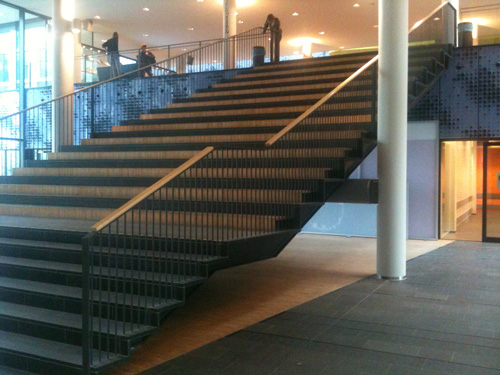
\includegraphics[width=0.4\linewidth]{images/exp2-stair-photo.jpg}
\caption{Photo of the stair which is traversed by the AR.Drone. The depth of each step is $30\small{cm}$ and the height of each step is $18\small{cm}$. The total height of the stair is $480\small{cm}$.}
\label{fig:exp2-stair-photo}
\end{figure}

The results of this experiment can be found in Figure \ref{fig:exp2-results}.
After fully traversing the stair, the measured elevation is $313\begin{small}cm\end{small}$ and the error is $\frac{480 - 313}{480} \times 100 = 35\%$.
The shape of the measured elevation (Figure \ref{fig:exp2-results}) corresponds with the shape of the stair (Figure \ref{fig:exp2-stair-photo}).
However, the approach underestimates the elevation.
When traversing the stair, the AR.Drone's altitude stabilization increases the altitude smoothly, which causes a continuous altitude increase.
Therefore, the observed altitude difference within an elevation event is smaller than the actual altitude different caused by an object.
Another explaination of the underestimation is the error in the triggering of elevation events (due to thresholds).
When an elevent event is triggered at a suboptimal timestamp, the full altitude difference is not observed.
Ideally, an elevation UP event is triggered right before an object is detected by the ultrasound sensor, and an elevation NONE event is triggered right after the full height of the object is observed by the ultrasound sensor.


\begin{figure}[htb!]
  \begin{center}
    \subfigure[Plot of the detected elevation]{\label{fig:exp2-stair-plot}%
	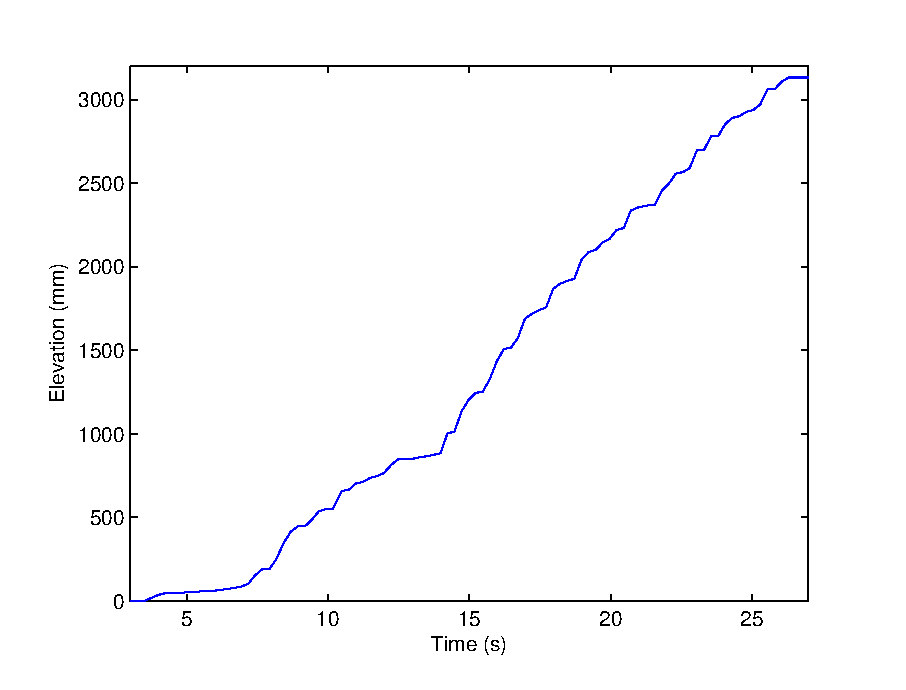
\includegraphics[width=0.55\linewidth]{images/exp2-stair-elevation-plot.eps}}%
    \subfigure[Visual elevation map]{\label{fig:exp2-stair-map}%
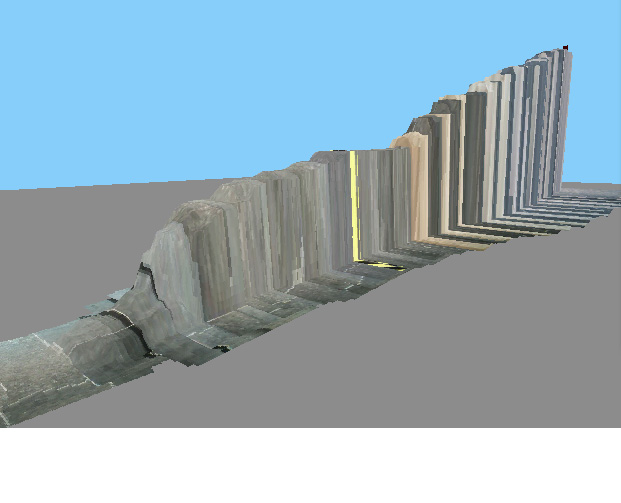
\includegraphics[width=0.4\linewidth]{images/exp2-stair-map.jpg}}

 \end{center}
  \caption{Elevation map of a large stair (Figure \ref{fig:exp2-stair-photo}). In \ref{fig:exp2-stair-plot} the measured elevation is plotted over time. In \ref{fig:exp2-stair-map} the elevation map is rendered using the 3DTerrain component of the presented framework.}
  \label{fig:exp2-results}
\end{figure}

\subsubsection{Elevation map of multiple objects}

In the second experiment, the elevation mapping approach is evaluated in terms of error in the estimated dimensions of objects.
Objects with different dimensions were laid out on a flat floor.
A photo of the floorplan can be found in Figure \ref{fig:exp2-setup}.
The AR.Drone's trajectory, which covers all objects, is indicated with a red line.
% and the object's dimensions 
%The AR.Drone flew the marked trajectory over all objects.

\begin{figure}[htb!]
\centering
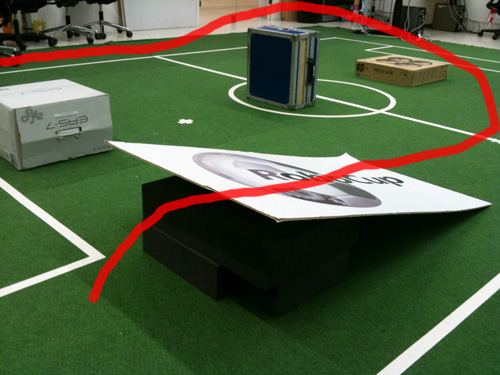
\includegraphics[width=0.4\linewidth]{images/exp2-elevation-setup.jpg}
\caption{Photo of the floorplan with different objects. The dimensions of the objects can be found in Table \ref{tab:exp2}. The red line indicates the trajectory of the AR.Drone.}
\label{fig:exp2-setup}
\end{figure}

The results of this experiment can be found in Table \ref{tab:exp2} and Figure \ref{fig:exp2-2-results}.
An object's width is evaluated in the trajectory's direction only. 
For the other direction, the width of an object cannot be estimated accurately, because the refinement step from Section \ref{sec:elevation_map} cannot be applied.


\begin{table}[htb!]
    \centering
    \begin{tabular}
        { | l | l | l | l | l | } 
	\hline
	Object & Dimensions (w$\times$h) (\small{mm}) & Estimated dimensions & Absolute error & Relative error \\
        \hline
        1. White box	& 460 $\times$ 290	& 390 $\times$ 245	& 70 $\times$ 45	& \textbf{15 $\times$ 16 \%}\\
	2. Blue box	& 245 $\times$ 490	& 250 $\times$ 420	& 5 $\times$ 70	& \textbf{2 $\times$ 14 \%}\\
	3, Brown box	& 570 $\times$ 140	& - 					& - 				& - \\
	4. Ramp		& 1380 $\times$ 360	& - 					& - 				& - \\
	\hline
    \end{tabular}
    \caption{Errors made in the estimated dimensions of objects. The first dimension is the width of an object in the y-direction and the second dimension is the height of an object. }
    \label{tab:exp2}
\end{table}

The white and blue boxes are detected.
The errors of both the estimated width and height are small.
Similar to the previous experiment, the height of an object is (slightly) underestimated.
The width of the white box is underestimated, which is probably caused by unreliable velocity estimates due to the lack of sufficient features.
Another explaination could be that the visual odometry methods assume a flat world, which does not hold when flying above objects.
Between both boxes, a false elevation is detected (clearly visible in Figure \ref{fig:exp2-elevation-plot}).
This elevation is probably triggered by an aggressive descent, caused by the AR.Drone's altitude stabilization, after the white box is passed.

The brown box is not detected due its limited height.
Therefore, the measured (ultrasound) acceleration is unsufficient to trigger an elevation event.
As expected, the ramp was not detected.
The gradual elevation change does not produce a significant acceleration.

\begin{figure}[htb!]
  \begin{center}
    \subfigure[Plot of the detected elevation]{\label{fig:exp2-elevation-plot}%
	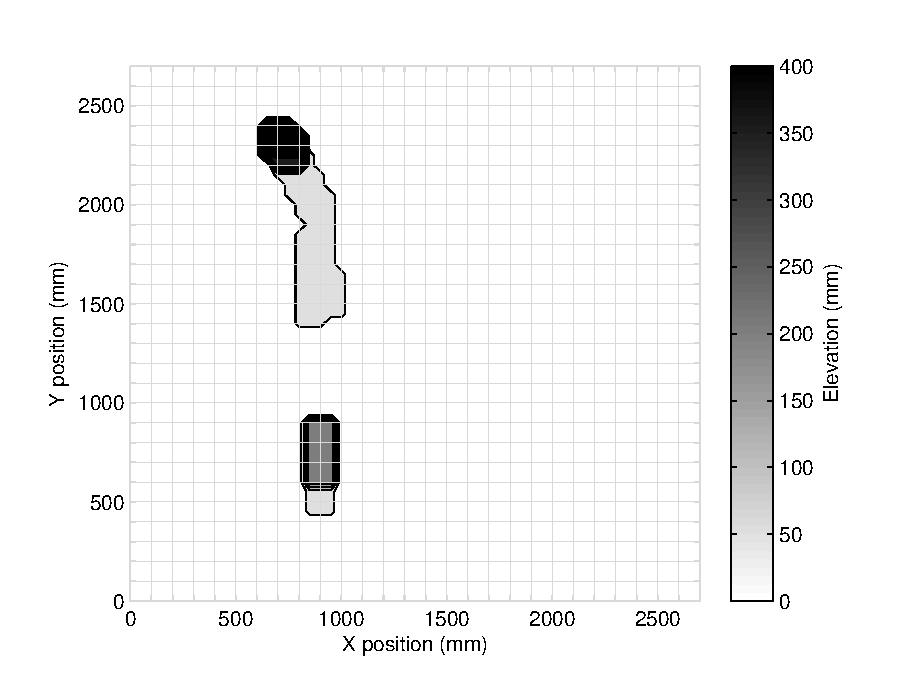
\includegraphics[width=0.55\linewidth]{images/exp2-contourf.eps}}%
    \subfigure[Visual elevation map]{\label{fig:exp2-elevation-map}%
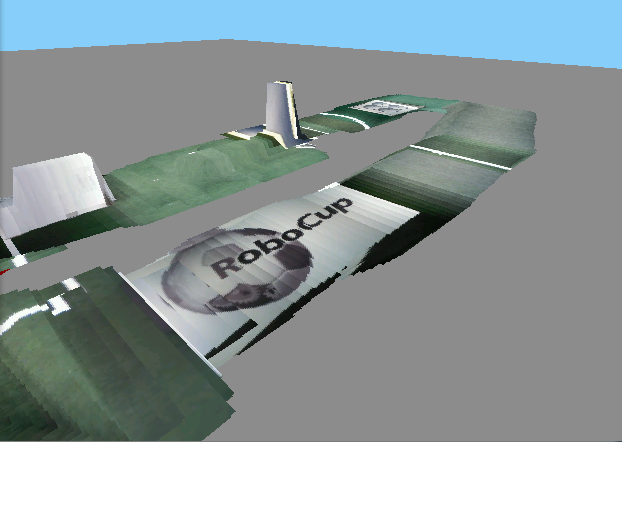
\includegraphics[width=0.4\linewidth]{images/exp2-elevation-map.png}}

 \end{center}
  \caption{Elevation map of multiple objects (Figure \ref{fig:exp2-setup}). In \ref{fig:exp2-stair-plot} a contour map of the elevation is plotted. In \ref{fig:exp2-stair-map} the elevation map is rendered using the 3DTerrain component of the presented framework.}
  \label{fig:exp2-2-results}
\end{figure}



%\chapter{Discussion}
%\label{chapter:discussion}
%\textbf{TODO}



\chapter{Conclusions}
\label{chapter:conclusions}
This chapter concludes this thesis by summarizing its content and answering the research questions.
Section \ref{sec:conclusions-contributions} describes the contributions of this thesis.
Finally, Section \ref{sec:conclusions-future} motivates several interesting directions for future research.

The platform selected in this thesis is the Parrot AR.Drone quadrotor helicopter.
A simulation model of the AR.Drone is proposed, which allows safe and efficient development of algorithms.
This simulation model consists of a motion model, visual model and sensor model.
The validation effort of the hovering and the forward movement shows that the dynamic behavior of the simulated AR.Drone closely resembles the dynamic behavior of the real AR.Drone.

A framework is proposed to perform high-level tasks with the AR.Drone.
This framework includes an abstraction layer to abstract from the actual device, which allows to use both the real and simulated AR.Drone to test the proposed methods.
The framework stores video frames and sensor measurements from the AR.Drone in queues, such that algorithms can operate on the data.
Furthermore, the framework includes a 3D map visualization and provides functionalities to record and playback data.

This thesis proposed a real-time Simultaneous Localization and Mapping approach that can be used for micro aerial vehicle with a low-resolution down-pointing camera (e.g., AR.Drone).
The information from the sensors are used in an Extended Kalman Filter (EKF) to estimate the AR.Drone's pose.
The position of the AR.Drone cannot be estimated directly and is derived from the velocity estimates from the AR.Drone.
This estimate is based on the inertia measurements, aerodynamic model and visual odometry obtained from the relative motion between camera frames.
When an estimate of the AR.Drone's pose is available, a map can be constructed to make the AR.Drone localize itself and reduce the error of the estimated pose.
The map consists of a texture map and a feature map.
The texture map is used for human navigation and the feature map is used by the AR.Drone to localize itself.

The texture map is constructed by warping a camera frame on a flat canvas.
A homography matrix describes how each frame has to be transformed (warped) in order to generate a seamless texture map without perspective distortion.
For each frame, the estimated pose and camera matrix are used to determine the area of the world which is observed by the camera.
This area is described by four 2D coordinates (a flat world is assumed).
Now, the homography is estimated from the four 2D world positions and their corresponding frame's pixel coordinates.

The feature map consists of a grid with SURF features.
For each camera frame, SURF features are extracted.
The estimated pose and camera matrix are used to compute the 2D world position of each feature.
Based on the 2D world position, a feature's cell inside the grid is computed.
Only the best feature of a cell is stored.

This feature map is used by the AR.Drone to localize itself.
For each camera frame, SURF features are extracted.
Similar to the mapping approach, the corresponding 2D world position of each feature is computed.
Each feature is matched against the most similar feature from the feature map.
From the feature pairs, a robust transformation between the 2D world coordinates is estimated.

An approach is proposed to compute the transformation between a frame and a map.
The method is very similar to RANSAC, but uses covariance instead of the number inliers as quality measure.
Three random feature pairs are selected.
From these pairs, the 2D world coordinates are used to compute the mean translation.
The covariance describes the quality of a translation.
These steps are repeated multiple times and the best translation is selected.
If a translation is very good (i.e., low covariance), Kabsch algorithm is used to refine the AR.Drone's estimated rotation.
Experiments show that the proposed method significantly outperforms OpenCV's implementation to estimate a perspective, affine or Euclidean transformation.
By reducing the degrees of freedom and using a beter quality measure, the robustness against noise increases.

A slightly modified version of the localization approach is used to perform visual odometry (estimate the velocity from camera images).
Instead of matching the last frame against the feature map, now the last frame is matched against the previous frame.
This estimated velocity can be used instead 
% or in combination with
 the AR.Drone's onboard velocity estimate.
Experiments show that the accuracy of the proposed visual odometry method is comparable to the AR.Drone's onboard velocity estimate.

Experiments show the AR.Drone down-pointing's camera offers good balance between image quality and computational performance.
When the resolution of the AR.Drone's camera is reduced, the accuracy of the estimated position decreases.
The reduced image quality results in less frames that could be used to robustly recover the velocity.
A simulated AR.Drone was used to investigate an increased camera resolution.
An increased image resolution does not necessarily produce more accurately estimated positions.
While relatively more frames could be used to used to robustly recover the velocity, the absolute number of processed frames decreased due to the increased computational complexity.
Therefore, the velocities are estimated less frequent.

Another experiment shows that localization is possible for circumstances encountered during the IMAV competition.
When flying the figure-8 shape three times, the maximum error was $1\small{m}$.
During a flight of $x\small{s}$, the visual odometry was recovered $x$ times, and localization against a map was performed $x$ times.

In addition to the texture and feature map, this thesis proposed a method to construct an elevation map using a single airborne ultrasound sensor.
Elevations are detected through sudden changes in ultrasound measurements.
These sudden changes are detected when the filtered second order derivative exceeds a certain threshold.
Experiments show that the relative error when flying over small objects is below $20\%$.
When flying over a large staircase, the relative error in estimated altitude was $35\%$.









\section{Contributions}
\label{sec:conclusions-contributions}

The first contribution of this thesis is a framework that aids in the development of (intelligent) applications for the AR.Drone.
The framework contains an abstraction layer to abstract from the actual device and use a simulated AR.Drone in a way similar to the real AR.Drone.
Therefore, a simulation model of the AR.Drone is developed in USARSim.
The main contribution is a novel approach that enables a MAV with a low-resolution down-looking camera to navigate in circumstances encountered during the IMAV competition.
An algorithm is presented to estimate the transformation between a camera frame and a map.
In addition to the navigation capabilities, the approach generates a texture map, which can be used for human navigation.
Another contribution is a method to construct an elevation with a single airborne ultrasound sensor.

\section{Future research}
\label{sec:conclusions-future}
%This thesis provides a broad range of directions for future research.

The proposed simulation model of the AR.Drone is validated in terms of hovering and forward movements. 
Further improvements would require more system identifications (e.g., rotational movements, wind-conditions) and include the characteristics of the Parrot's proprietary controller into the simulation model. 
The current sensor model uses a set of default USARSim sensors, which do not model noise accurately.
This research would benefit from a realistic modeling of the noise in the sensors.

The proposed SLAM method is able to construct a map and localize the AR.Drone in real-time.
However, the proposed method lacks a global map optimization method, which reduces the error in the map when a loop-closure is detected.
An interesting research direction is to develop a global map optimization that is able to optimize both the feature map and texture map in real-time.

Experiments have shown that the proposed visual odometry method is unable to accurately estimate the velocity when insufficient texture is visible on the floor.
In these circumstances, the AR.Drone's onboard optical-flow based visual odometry method is able to estimate the velocity more accurately.
However, salient lines on the floor cause the AR.Drone's optical-flow method to estimate the velocity in the wrong direction.
This problem can be solved by integrating additional information (e.g., aerodynamic model) into the optical-flow method, to correct the direction of the estimated velocity.
When such a method is incorporated in the proposed SLAM method, it would yield an increased accuracy of the estimated velocities in low-texture conditions.

The elevation mapping experiment has shown that elevation mapping with a single ultrasound sensor is possible.
However, the proposed method is sensitive to errors that accumulate.
When an object is detected, the elevation is increased.
When an object is out of range, the elevation is decreased.
When both events do not observe an equal elevation, an incorrect elevation propagates into the elevation map.
A possible solution could be a global optimization method, which is able to correct incorrect elevations.
For example, large areas for which the elevation does not change can be assumed to be the floor.
Furthermore, the current approach is unable to estimate the dimensions of an object in all directions.
Visual clues could be used to estimate the dimensions of an object.
For example, image segmentation can be used to determine the boundaries of an object.
Another possible solution is to create a depth map from optical flow.
Just as stereo vision can be used to create a depth map of the environment, the optical flow between two subsequent frames can be used to create a depth map \cite{Jurriaans2011}.

The proposed framework uses a single thread to process the camera frames.
Therefore, the proposed SLAM method is unable to benefit from an increased image resolution.
This issue can be solved by processing multiple frames in parallel (using multiple video processing threads), to make better use of a multicore CPU.



\appendix
\chapter{Opening angle of the ultrasound sensor}
\label{appendix:opening_angle}

The opening angle of the AR.Drone's ultrasound sensor is not documented.
A small experiment has been performed to determine the opening angle.

The AR.Drone was positioned at a fixed altitude of $79\small{cm}$ above a flat floor.
No obstacle was in range of the ultrasound sensor to make sure the measured altitude is the actual altitude of the AR.Drone.
The altitude measured by the ultrasound sensor was $75.2\small{cm}$, which equals a systematic error of $3.8\small{cm}$.
The AR.Drone's bottom camera was used to mark a point on the floor that is exactly below the center of the AR.Drone.
This point is equal to the center of ultrasound cone.
In order to measure the opening angle, floating objects were moved from outside the cone towards the cone.
The objects require a certain distance from the floor to achieve a distance short than the shortest distance between the sonar and the floor.
The minimal altitude of an object when assuming a maximum opening angle of $40$ degrees is:
\begin{equation}
a = 79\small{cm} - (cos(40\deg) \times 79\small{cm}) = 18.48\small{cm}
\end{equation}
Fluctuations in the altitude measurements indicate that the object is entering the cone.
The horizontal distance $d$ between the object and cone center (marked point) is the width of the cone and $h = 79\small{cm} - a$ is the height of the cone.
The angle $\alpha$ of the cone can be recovered with:
\begin{equation}
\alpha = tan^{-1}(d / h)
\end{equation}

The experiment was repeated $10$ times with different objects.
The average opening angle is $25.03^{\circ}$ with a standard deviation of $1.45^{\circ}$.





\chapter{Source code}
All source code is available at Google Code: \url{http://code.google.com/p/mscthesis-ndijkshoorn/}.
The recorded datasets, which are stored in YAML format, can be found at the downloads page: \url{http://code.google.com/p/mscthesis-ndijkshoorn/downloads/list}.

A research log can be found at \url{http://nickd.nl/wiki/thesis}.

\begin{figure}[htb]
\centering
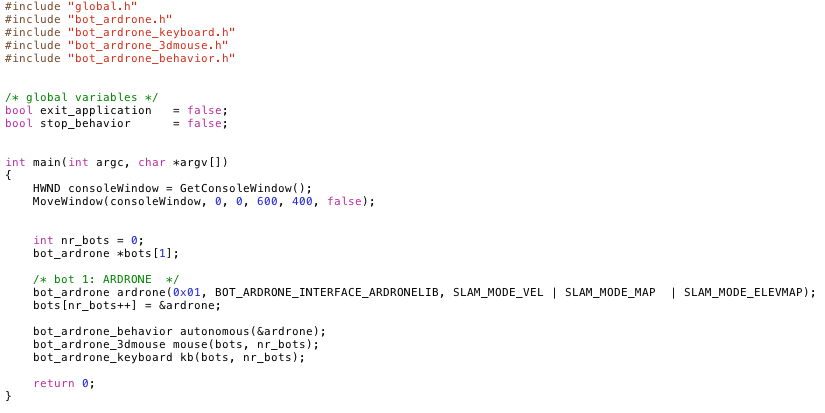
\includegraphics[width=\linewidth]{images/screenshot-code.png}
\caption{Source code of the application main file. This code initializes a robot instance and its controllers (autonomous behavior, keyboard and 3D mouse).}
\end{figure}

\linespread{1.0}
\bibliographystyle{mystyle}
%\bibliographystyle{unsrt}
%\vspace{0.3in}
\bibliography{references}

\end{document}